\documentclass[12pt,a4paper]{report} 
\usepackage[greek,italian]{babel} 
\usepackage{amsmath}
\usepackage{latexsym} 
\usepackage{newlfont} 
\usepackage{color} 
\usepackage{setspace}
\usepackage{eqnarray}
%\usepackage{makeidx}
\usepackage{graphicx} 
\usepackage{amsmath}
\usepackage{wrapfig}
\usepackage{fancyhdr} 
\textwidth=450pt
\oddsidemargin=0pt 


\begin{document}
%%%%%%%%%%%%%%%%%%%%%%%%%%%%%%%%%%%%%%%%%%%%%%%%%%%%%%

%\frontmatter
\begin{titlepage}
\begin{center}
\begin{figure}[h!]
\centering
\includegraphics[width=5cm]{logo_verticale_2.pdf}
\end{figure}
{\large Universit\'a degli Studi di Siena}\\
\vspace{2mm}
{\large {Dipartimento di Scienze Fisiche, della Terra e dell'Ambiente}}\\
\vspace{10mm}
{\large Corso di laurea in Fisica e Tecnologie Avanzate}\\
\vspace{10mm}
\vspace{7mm}
\Large{\bf{SIMULAZIONE MONTE CARLO 

DI SCATTERING INELASTICO $pp$ A  $\sqrt{s}=13$ TeV CON CT-PPS}}
\end{center}
\vspace{20mm}
\begin{tabular}{@{}ll@{}}
{\large {Relatore:}} & {\large {Nicola Turini}}\\
\end{tabular}
%\vspace{10mm}
\begin{flushleft}
\hspace{11cm}{\large {Tesi di Laurea di}}\\ \vspace{2mm}
\hspace{11cm}{\large {Lorenzo Marini}}\\ \vspace{2mm}
\end{flushleft}
\vspace{4mm}
\centering
{\large \sl{Anno Accademico 2017/2018}}
\end{titlepage}



%%%%%%%%%%%%%%%%%%%%%%%%%%%%%%%%%%%%%%%%%%%%%%%%%%%%%%
\tableofcontents{}

\listoffigures
%\listoftables

%%%%%%%%%%%%%%%%%%%%%%%%%%%%%%%%%%%%%%%%%%%% 
\pagestyle{headings}
\onehalfspacing %interlinea, lascia pi� spazio tra le righe

 
\chapter*{Introduzione}
\addcontentsline{toc}{chapter}{Introduzione}
\chaptermark{Introduzione}

TOTEM \'e un esperimento situato presso il Large Hadron Collider del CERN, il pi\'u grande acceleratore di particelle al mondo, che attualmente fornisce dati su collisioni protone-protone ad una energia del centro di massa di 13 TeV.\newline
Lo scopo principale di questo esperimento \'e stato quello effettuare la misura della sezione d'urto totale con precisione del 1 $\div$ 2 $\%$, studiare diffusione elastica e delle interazioni inelastiche nelle collisioni protone-protone. 

Dal 2017 TOTEM partecipa inoltre ad un pi\'u completo programma di fisica diffrattiva in collaborazione con CMS, l'altro esperimento presente nel tunnel di LHC al punto di interazione IP5 (esperimento CT-PPS).\newline
Durante la mia permanenza al CERN ho avuto l'opportunit\'a di lavorare presso la collaborazione CMS-TOTEM contribuendo allo sviluppo di una macro di ROOT, il cui codice \'e scritto in linguaggio C++, finalizzato alla simulazione della cinematica di uno scattering inelastico protone-protone.

La presente tesi \'e strutturata in 4 capitoli:
\begin{description}
\item[ ] nel capitolo 1 viene introdotto l'acceleratore LHC assieme ad una panoramica pi\'u nel dettaglio dell'esperimento CT-PPS (Precision Proton Spectrometer): dai rivelatori utilizzati alle condizioni sperimentali. In particolare nella prima parte vi \'e una presentazione dei Roman Pot, mentre nella seconda \'e presentata una discussione sull'ottica del fascio, sull'accettanza e la risoluzione dei rivelatori;
\item[ ] il capitolo 2 tratta del programma di fisica dell'esperimento CT-PPS, riguardante essenzialmente fenomeni di fisica diffrattiva (produzione centrale esclusiva $WW$, $dijets$ e collisioni a due fotoni). Nella parte finale di questo capitolo vi \'e inoltre un'introduzione pi\'u in generale ai processi elastici, diffrattivi e inelastici;
\item[ ] nel capitolo 3 analizzeremo la cinematica di uno scattering inelastico tra protoni in trattazione relativistica. L'obiettivo di tale studio sar\'a quello di ricavare le espressioni analitiche delle grandezze del moto da implementare, in un secondo momento, nel codice di simulazione;
\item[ ] infine nel capitolo 4 vengono descritte e spiegate le parti pi\'u importanti del codice e mostrate le distribuzioni da questo generate (i.e. impulso trasverso, angolo di scattering, psuedorapidit\'a ecc.). 

Per concludere nella parte finale del capitolo sono presentate le simulazioni delle distribuzioni spaziali dei protoni misurate dai Roman Pot.
\end{description}


%%%%%%%%%%%%%%%%%%%%%%%%%%%%%%%%%%%%%%%%%%%%%%%%%%%%%%%%%%%%%%%%%%%%%%%%%%%%%%%
\chapter{L'esperimento CT-PPS a LHC}
Nei primi anni 50 in Europa venne fondato il CERN (Centro Europeo per la Ricerca Nucleare), un istituto che mirava a promuovere la collaborazione a livello europeo nella ricerca scientifica. Da allora molti progressi sono stati fatti nella comprensione dei fenomeni della fisica atomica, nucleare e sub-nucleare.
Nel sito del CERN, al confine tra la Svizzera e la Francia, sono stati col tempo costruiti acceleratori di particelle sempre pi\'u grandi e potenti, in grado di operare ad energie sempre maggiori per investigare il mondo microscopico pi\'u a fondo.
Oggi questi acceleratori costituiscono un unico complesso (Fig. 1.1) capaci di incrementare la velocit\'a e quindi l'energia di particelle di vario genere (protoni, antiprotoni, elettroni, ioni, etc.).   


\begin{figure}[h] 
\centering 
\includegraphics[scale=0.4]{LHC.pdf} 
\caption{Complesso degli acceleratori del CERN.} 
\end{figure}
 %%%%%%%%%%%%%%%%%%%%%%%%%%%%%%%%%%%%%%%%%%%%
\section{Large Hadron Collider}

Entrato in funzione il 10 settembre 2008 LHC \'e attualmente il pi\'u grande acceleratore di particelle al mondo, in grado di raggiungere un'energia del centro di massa ($\sqrt{s}$) di 14 TeV. Nel tunnel sotterraneo di 27 Km, che ha ospitato il Large Electron Positron Collider (LEP) fino all'anno 2000, sono stati posti i magneti superconduttori che lo costituiscono.


\begin{figure}[h] 
\centering 
\includegraphics[scale=0.4]{LHCTunnel.pdf} 
\caption{Tunnel di LHC.} 
\end{figure}

All'interno di caverne artificiali situate a circa 100 metri di profondit\'a si trovano gli apparati sperimentali (ALICE, ATLAS, CMS, LHCb, LHCf, TOTEM) capaci di raccogliere i dati sulle collisioni protone-protone, protone-ione e ione-ione realizzate da LHC.Infatti all'interno del tunnel viaggiano, in direzioni opposte, due fasci di protoni o ioni, i quali vengono fatti collidere con lo scopo di produrre fasci di particelle ad alta energia.
Con LHC \'e possibile indagare la fisica subnucleare a energia del TeV e ci\'o apre la strada alla ricerca in diversi ambiti, tra cui:

\begin{itemize}
\item Modello Standard e Meccanismo di Higgs
\item Materia oscura
\item Teorie Supersimmetriche (SUSY)
\item Plasma di Quark e Gluoni (QGP)
\item Extra dimensioni spaziali e temporali.
\end{itemize}


In LHC si studiano principalmente le collisioni protone-protone. Prima di entrare nel collisore circolare, i protoni devono attraversare un sistema di acceleratori che ne aumenta l'energia in modo graduale. Una volta iniettati nell'anello di LHC, essi entrano in direzione opposta in due linee adiacenti, costituite da tubi metallici circolari, al cui interno viene creato l'ultra-alto vuoto ($10^{-7}$ Pa). Affinch\'e le particelle seguano la corretta traiettoria, \'e montato un sistema di magneti: 1232 dipoli magnetici per mantenere la traiettoria circolare, e 392 quadrupoli magnetici per focalizzare il fascio.
\newline
Per mantenere i magneti in regime operativo di 1.9 gradi Kelvin si utilizza un sistema criogenico con $He_4$ superfluido.

Poich\'e le particelle perdono energia viaggiando su traiettorie circolari emettendo radiazione, lungo il percorso sono disposte cavit\'a acceleratrici a radiofrequenza (RF).


I protoni, ottenuti ionizzando atomi di idrogeno, vengono inizialmente accelerati fino a energie di 50 MeV dall'acceleratore lineare LINAC2, quindi sono iniettati nel PSBooster e successivamente nel Proton Synchrotron (PS) dove raggiungono un'energia di 26 GeV.

\begin{figure}[h] 
\centering 
\includegraphics[scale=0.6]{magnete.pdf} 
\caption{Sezione di un magnete dipolare di LHC.} 
\end{figure}
 Lo stadio successivo \'e il Super Proton Synchrotron (SPS), un anello di 2 Km di diametro che porta i protoni a 450 GeV prima di immetterli infine nel Large Hadron Collider. I fasci di protoni sono accelerati fino a velocit\'a prossime a quelle della luce e vengono fatti circolare all'interno di due tubi a vuoto paralleli mediante dei magneti superconduttori raffreddati dall'Elio liquido.
In figura 1.3 \'e rappresentata la sezione di un magnete dipolare.

Tali magneti super conduttori sono in grado di generare un campo magnetico di 8.33 Tesla che permette la curvatura dei fasci. 
Le cavit\'a a radiofrequenza accelerano i fasci fino al 99,999999 $\%$ della velocit\'a della luce, mentre i quadrupoli magnetici restringono ad ogni passaggio la sezione del fascio. 
%%%%%%
In LHC i protoni acquistano un'energia di 7 TeV e vengono raggruppati in 2800 pacchetti, detti $bunches$, contenenti pi\'u di 100 miliardi di particelle per pacchetto. 
\newline
I pacchetti di protoni che viaggiano in direzione opposta all'interno dei tubi a vuoto vengono fatti collidere in quattro punti di interazione in una camera a vuoto.
Le collisioni avvengono ogni 25 $ns$ producendo in media 20 eventi di collisione protone-protone; la luminosit\'a \'e di $10^{34}$ $cm^{-2}s^{-1}$[3]. 
\begin{figure}[h] 
\centering
\includegraphics[scale=0.46]{schema_LHC.pdf} 
\caption{Schema di LHC.}
\end{figure}

Nei quattro punti in cui i fasci collidono sono posizionati i principali esperimenti, ognuno dei quali utilizza metodi e tecniche diverse: ATLAS (A Toroidal LHC Apparatus), ALICE (A Large Ion Collider Experiment), LHCb (LHC beauty), CMS (Compact Muon Solenoid).
\newline


%%%%%%%%%%%%%%%%%%%%%%%%%%%%%%%%%%%%%%%%%%%%

\section{CMS - TOTEM Precision Proton Spectrometer}
La sfida principale del programma sperimentale CT-PPS \'e la capacit\'a di azionare i rivelatori vicino al fascio (10-20 $\sigma$) ad alta luminosit\'a. Infatti per massimizzare l'accettanza dei protoni a bassa perdita di momento i rivelatori devono operare a distanze di pochi mm dal centro del fascio ed essere attivi il pi\'u vicino possibile al loro bordo fisico.\newline
In questo capitolo viene descritta la progettazione tecnica e delineate le prestazioni attese dello spettrometro di precisione dei protoni di CMS-TOTEM (CT-PPS). \newline
CT-PPS aggiunge rivelatori di tracking e di timing nella regione molto pi\'u in avanti su entrambi i lati di CMS a circa 200 m dal punto di interazione (IP) per studiare la produzione esclusiva centralizzata (CEP) nelle collisioni protone-protone.

CEP fornisce un metodo unico per accedere a una variet\'a di temi di fisica ad alta luminosit\'a a LHC, come la nuova fisica riguardante la produzione di nuove risonanze, la produzione di jet ad alto potenziale e la produzione anomala di coppie di bosoni $W$ e $Z$.

Il rivelatore CT-PPS consiste in un sistema di rivelatori di tracciamento di silicio per misurare la posizione e la direzione dei protoni e un set di contatori temporali per misurare il loro tempo di arrivo con una precisione dell'ordine di 10 ps. Ci\'o a sua volta consente la ricostruzione della massa, della quantit\'a di moto e della coordinata $z$ del vertice primario del sistema prodotto centralmente.

Il framework per lo sviluppo e l'utilizzo di CT-PPS \'e definito in un $Memorandum$ $of$ $Understanding$ firmato dal CERN e dalla collaborazione CMS e TOTEM.

\subsection{Panoramica sullo spettrometro di precisione per protoni CMS - TOTEM}
Per studiare la produzione esclusiva centrale in collisione protone-protone, ovvero il processo $pp$ $\rightarrow$ $pXp$, in cui i protoni non si dissociano e interagiscono tramite fotone o scambio di colori per produrre il sistema $X$ nella regione centrale, sono utilizzati tracking e timing detector nella regione pi\'u avanti su entrambi i lati di CMS.

Il CMS-TOTEM Precision Proton Spectrometer (CT-PPS) \'e uno spettrometro magnetico che utilizza i magneti di LHC tra il punto di interazione (IP) e le stazioni di rivelamento a $\sim$ 210 m dall'IP su entrambi i lati, per deflettere i protoni che hanno perso una piccola frazione del loro impulso fuori dal fascio in modo tale che le loro traiettorie possano essere misurate.

La disposizione del fascio nella regione posta 210 m dopo il primo Long Shutdown (LS1) \'e mostrata in figura 1.6.

\begin{figure}[h] 
\centering
\includegraphics[scale=0.42]{pps.pdf} 
\caption{Layout dei rivelatori CT-PPS nella regione 210 m dopo LS1. I Roman Pot cilindrici sono dotati di timing detector per il rifiuto dell'unit\'a PU. I Roman Pot (RP) a forma di scatola sono dotati di rivelatori di pixel per misurare lo spostamento dei protoni scatterati dal fascio.}
\end{figure}

La produzione esclusiva centralizzata (CEP) fornisce un metodo unico per accedere a una variet\'a di argomenti di fisica, come la nuova fisica riguardante la produzione anomala di coppie di bosoni $W$ e $Z$, produzione di $jet$ ad alto momento trasverso ($p_T$) ed eventualmente la produzione di nuove risonanze.

Questi studi possono essere condotti in condizioni sperimentali particolarmente pulite grazie all'assenza di residui dei protoni. La rilevazione dei due protoni di stato finale, deviati a quasi zero gradi, in rivelatori molto vicini al fascio, fornisce una firma sorprendente. La misurazione dei protoni primari consente di determinare completamente la cinematica del sistema centrale. Gli stati finali ben definiti nel rivelatore centrale di CMS, assieme alla cinematica dei protoni, possono quindi essere selezionati e ricostruiti con precisione.

Inoltre un certo numero di studi di fisica sar\'a finalizzato alla comprensione dei meccanismi di QCD coinvolti nella CEP, come per esempio la produzione esclusiva con $M(jj)$ fino a $\sim$ 700 - 800 GeV, che consente lo studio di campioni di jet di gluone puro con una piccola contaminazione di jet di quark.
\newline

Uno dei motivi per cui CEP \'e particolarmente interessante consiste nel fatto che se i protoni in uscita rimangono intatti e si propagano con piccoli angoli di scattering, allora con una buona approssimazione, il sistema dei gluoni obbedisce a una regola di selezione su $J_z$. Questa regola di selezione consente una determinazione pulita dei numeri quantici di ogni nuova risonanza.

\subsection{Rivelatori e condizioni sperimentali}
I rivelatori di CT-PPS operano a pochi mm dal fascio durante l'acquisizione dei dati. In ogni braccio sono installate, a dieci metri di distanza lungo l'asse $z$, due stazioni di tracciamento con sensori di pixel resistenti alle radiazioni e sono seguite dalle stazioni di temporizzazione.
Le stazioni sono installate lungo la linea del fascio, tra 204 e 215 m dall'IP (regione gi\'a utilizzata da TOTEM). A valle dei rivelatori \'e presente un collimatore (TCL6) per proteggere il quadrupolo Q6 dallo sciame di particelle originate nei rivelatori CT-PPS.
\newline
Il tracking di CT-PPS \'e progettato per la risoluzione della posizione di circa 10 (30) $\mu$m e una risoluzione angolare di 1 (3) $\mu$rad nel piano $x-z$ ($y-z$). In ogni braccio il rivelatore di tracciamento \'e formato da due RP con sei strati di pixel ciascuno. Ogni livello include un sensore di 16 x 24 ${mm}^2$ pixel abbinato a sei PSI46 front-end ASCI e un Token Bit Manager (TBM). I sensori di pixel in silicio 3D sono stati scelti come base di riferimento di CT-PPS per la loro superiore resistenza alla radiazione.

Gli studi basati sulle frequenze rilevate dal rivelatore TOTEM e sulle simulazioni indicano flussi di particelle fino a 45 x $10^{15}$ ${cm}^{-2}$ per 100 ${fb}^{-1}$ nei rivelatori a pixel. \newline
Una descrizione pi\'u dettagliata dei rivelatori di tracciamento \'e presentata nel paragrafo 1.2.3. Infine in entrambe le braccia i rivelatori di temporizzazione misurano la differenza del tempo di arrivo dei due protoni. Una risoluzione temporale di $\sigma$(t) = 10 ps corrisponde a una risoluzione di vertice $\sigma$($z_{pp}$) = 2.1 mm.
\newline

Studi basati su monitor di radiazione collocati sulle stazioni dei RP di TOTEM (a 220 metri) producono una dose totale di circa 100 Gray e una fluenza dell'ordine di $10^{12}$ neq/${cm}^2$ per 100 ${fb}^{-1}$ di luminosit\'a integrata.
 
\subsection{Il sistema dei Roman Pot e dei collimatori nella regione di IP5 a 200 m}

Nell'ambito del progetto CT-PPS, la linea del fascio nella regione di LHC distante \newline
$\pm$ 200 m da IP5 combina le stazioni RP220 m (220-Near, 220 -Far), le stazioni a 147 m (210-Near, 210-Far) e le nuove stazioni di timing RP (Figura 1.6).
Le unit\'a poste a 210 m sono ruotate di 8 gradi rispetto alla linea del fascio per migliorare la risoluzione multitraccia (Figura  1.8).

Durante LS1, i RP verticali a 210 m e tutti i RP a 220 m sono stati equipaggiati con telai meccanici di supporto migliorati per compensare l'espansione termica e consentire il rilascio di sollecitazioni meccaniche. \newline
La figura 1.7 mostra la beamline nel Settore 4-5 con in RP installati.   
\begin{figure}[h!] 
\centering
\includegraphics[scale=0.4]{Romanp1.pdf} 
\caption{Layout dei rivelatori CT-PPS nella regione a 200 m dopo LS1.}
\end{figure}
\newpage
\begin{figure}[t!] 
\centering
\includegraphics[scale=0.4]{Romanp3.pdf} 
\caption{La beamline nel settore 4-5 con i RP installati.}
\end{figure}
\begin{figure}[h!] 
\centering
\includegraphics[scale=0.5]{Romanp2.pdf} 
\caption{Rappresentazione delle unit\'a RP ruotate. Il punto di vista \'e diretto lungo il fascio in uscita.}
\end{figure}

\subsection{Ottica del fascio}
I tracking detector e timinig detector devono essere installati nelle regioni approssimativamente a $z$ = 204 m e $z$ = 215 m dall'IP, in entrambe le direzioni del fascio, rispetto al rivelatore centrale. I protoni che hanno perso energia nell'interazione primaria emergono lateralmente dopo aver attraversato i magneti di curvatura. A $z$ = 204-215 m si possono rivelare protoni che hanno perso una piccola percentuale ($\simeq$ 3 - 20 $\%$) dell'energia iniziale del fascio.
\newline

La traiettoria dei protoni prodotta con la posizione trasversale ($x^{*}$, $y^{*}$) e \newline
l'angolo (${\theta^{*}}_x$, ${\theta^{*}}_y$) nella posizione IP (l'apice '*' indica la posizione IP su IP5) \'e descritta dall'equazione:

\begin{equation}
\vec{d}= T \cdot \vec{d}^{*}
\end{equation}

dove il vettore $\vec{d}$ = ($x$, $\theta_{x}$, $y$, $\theta_{y}$, $\Delta$$p$/p) e $T$ \'e la matrice di trasporto; $p$ e $\Delta$$p$ indicano rispettivamente il momento del fascio e la perdita di momento longitudinale del protone. La matrice di trasporto \'e definita dalle funzioni ottiche come:
%%%%

\begin{equation}
T= \begin{pmatrix}
v_x & L_x & m_{13} & m_{14} & D_x\\
{v_x\over ds} & {L_x\over ds} & m_{23} & m_{24} & {D_x\over ds}\\
m_{31} & m_{32} & v_y & L_y & D_y\\
m_{41} & m_{42} & {v_y\over ds} & {L_y\over ds} & {D_y\over ds}\\
0 & 0 & 0 & 0 & 1\\
\end{pmatrix}
\end{equation}
\newline

dove la magnificazione $v_{x,y}$ \'e definita come

\begin{equation}
v_{x,y}=\sqrt{\beta_{x,y}/\beta^{*}}cos\Delta\phi_{x,y}
\end{equation}

e la lunghezza effettiva $L_{x,y}$
\begin{equation}
L_{x,y} = \sqrt{\beta_{x,y}/\beta^{*}}sin\Delta\phi_{x,y}.
\end{equation}

Entrambe sono funzioni dell'ampiezza di betatrone $\beta_{x,y}$ e della fase dall'IP al RP

\begin{equation}
\Delta\phi_{x,y} = \int_{IP}^{RP} {ds\over \beta (s)_{x,y}}.
\end{equation}

Queste, assieme alla dispersione $D_{x,y}$ (dove generalmente $D_y$ = 0), sono particolarmente importanti per la ricostruzione della cinematica dei protoni.
\newline Le figure che seguiranno fanno riferimento ad uno studio in cui l'energia del fascio dei protoni corrisponde a 6.5 TeV con LHC. 
\newline

La Figura 1.9 mostra i valori delle lunghezze effettive in $x$ e $y$ ($L_x$ e $L_y$) e le corrispondenti dispersioni ($D_x$ e $D_y$) in funzione di $\xi$ = $\Delta$$p$/$p$ (perdita di momento del protone sopravvissuto) sul rivelatore posizionato a $z$ = 204 m.


\begin{figure}[h!] 
\centering
\includegraphics[scale=0.5]{lunghezze.pdf} 
\caption{Lunghezze effettive in $x$ e $y$ ($L_x$ e $L_y$) e la corrispondente dispersione ($D_x$) in funzione della perdita di momento del protone $\xi$ in $z$ 204 m dal punto di interazione.}
\end{figure}

Questi valori, assieme all'ampiezza e alla divergenza del fascio, determinano l'accettanza e la risoluzione per le variabili cinematiche dei protoni $t$ (quadrimomento trasferito al quadrato) e $\xi$. Una volta iniziata la raccolta dati, le funzioni ottiche (e le loro risoluzioni) sono determinate dall'ottica del fascio effettivamente utilizzato, secondo il metodo discusso nell'articolo [2]. 
\newline

La configurazione della linea del fascio di LHC attorno all'IP di CMS \'e mostrata in Figura 1.10 per $z$ $>$ 0.

\begin{figure}[h!] 
\centering
\includegraphics[scale=0.48]{fascio.pdf} 
\caption{Vista dall'alto della linea del fascio per $z$ $>$ 0, con le traiettorie dei protoni simulate da HECTOR. Il punto di interazione \'e situato in $s$ = 0. La linea rossa (nera) corrisponde alle particelle entranti (uscenti) nell'IP. Qui la curva orizzontale \'e stata raddrizzata per chiarezza.}
\end{figure}

Il trasporto delle particelle dall'IP alla posizione del rivelatore di CT-PPS viene eseguito con HECTOR [3], il quale \'e incorporato nel package di simulazione e di ricostruzione del detector di CMSSW. I risultati dei recenti studi condotti sono in buon accordo con MAD-X [4], il programma standard di trasporto del fascio di LHC utilizzato al CERN.

Il package HECTOR traccia i protoni (o altre particelle) che emergono nella direzione in avanti dalla regione di interazione lungo la linea del fascio di LHC, simulata, insieme ai collimatori. Il trasporto del fascio pu\'o essere modificato per differenti configurazioni ottiche.

La dimensione del fascio pu\'o essere espressa in termini dell'emittanza $\epsilon$ e della funzione di ampiezza $\beta$. La dimensione orizzontale del fascio nel range della posizione del rivelatore di CT-PPS \'e mostrata in Figura 1.11. 


\begin{figure}[h!] 
\centering
\includegraphics[scale=0.53]{dimensione_fascio.pdf} 
\caption{Distanza orizzontale dal centro del fascio nella regione 220 $<$ $z$ $225$ m corrispondente alla posizione dei Roman Pot da 15$\sigma_x$ e 20$\sigma_x$. I parametri utilizzati per l'ottica sono descritti nel testo [6].}
\end{figure}

L'emittanza \'e inversamente proporzionale al momento del fascio; aumentando la quantit\'a di moto del fascio si riduce l'emittanza e quindi la dimensione fisica del fascio. Talvolta, viene spesso utilizzata l'emittanza normalizzata $\epsilon_n$ = $\epsilon$ $\beta$ $\gamma$ (dove $\beta$ e $\gamma$ sono funzioni relativistiche).

La funzione di ampiezza nell'IP assume il valore $\beta^{*}$ = 0.6 m, l'emittanza normalizzata $\epsilon_n$ $\simeq$ 3.75 x $10^{-6}$ (emittanza $\epsilon$ $\simeq$ 5.4 x $10^{-10}$) e un crossing angle di 142.5 $\mu$rad nel piano orizzontale. Si assume una risoluzione del vertice di $\sigma_{x,y}^{*}$ = 15 $\mu$m e una divergenza del fascio angolare di $\sigma^{*}$$\theta$ = 30 $\mu$rad all'IP [5].

\subsection{Accettanza e risoluzione dei rivelatori: $\xi$, t}

Le dimensioni dei rivelatori di CT-PPS (sia il timing che il tracking) sono limitate dallo spazio presente nei RP e determinano la copertura in $|t|$, $\xi$. In Figura 1.12 sono mostrate le distribuzioni in $x$ e $y$ dei protoni con valori fissi di ($|t|$, $\xi$) nelle due stazioni di tracciamento. Le distribuzioni sono ellissi centrate su $y$ = 0 e riflettono l'effetto dei magneti di quadrupolo lungo la linea del fascio. L'accettanza, per dati valori di ($|t|$, $\xi$), pu\'o essere stimata come la frazione della corrispondente ellisse coperta dai rivelatori. 
\newline

\begin{figure}[h!] 
\centering
\includegraphics[scale=0.43]{roman_simul.pdf} 
\caption{Particelle, con fissati valori di $|t|$ e $\xi$, propagate verso i rivelatori di CT-PPS posizionati a $z$ = 204 m (sinistra) e  $z$ = 215 m (destra). La linea nera continua (tratteggiata) rettangolare rappresenta i bordi del rivelatore a 15$\sigma$ (20$\sigma$) dal centro del fascio. Le dimensioni del fascio sono mostrate attraverso circonferenze. Per generare protoni a differenti valori di ($|t|$, $\xi$) si utilizza una simulazione "particle-gun" basata su HECTOR.}
\end{figure}

\newpage
Per quanto riguarda la distanza del rivelatore dal centro del fascio, viene utilizzato il seguente approccio: la RP window � posizionata a 15 (20) $\sigma$ dal centro del fascio e si assume che la distanza dei sensori da questa sia 0.3 mm. La regione morta aggiuntiva, a causa dell'inefficienza del bordo del sensore, non viene considerata; \'e stimato tra 0.1 mm e 0.2 mm, che corrisponde a 1 - 2$\sigma$ delle dimensioni del fascio.
\newline

Il rettangolo disegnato da una linea nera tratteggiata (solida) rappresenta i confini di un rivelatore con un'area (in $x$, $y$) di 20 x 18 ${mm}^2$ situata a 15$\sigma$ (20$\sigma$) + 0.3 mm dal centro del fascio, mentre gli inviluppi del fascio sono rappresentati schematicamente da ellissi centrate in zero.
Una risoluzione del rivelatore di 10 $\mu$m \'e rappresentata dallo smearing della posizione simulata del protone nella posizione del rivelatore.
 
Gli altri parametri chiave nel presente studio sono: la distanza dell'area sensibile del rivelatore dal centro del fascio e la risoluzione spaziale.
La distribuzione della collisione delle particelle \'e studiata per le dimensioni dell'area attiva a $z$ = 204 m e $z$ = 215 m, dove si assume che i piani del rivelatore siano ortogonali alla direzione del fascio. La segmentazione del rivelatore non \'e implementata nella simulazione, poich\'e ci si aspetta che questi abbiano un'area attiva finemente segmentata (la dimensione dei pixel in $x$, $y$ \'e $\approx$ 100 x150 $\mu$$m^2$).
\newline

\begin{figure}[h!] 
\centering
\includegraphics[scale=0.45]{sim.pdf} 
\caption{distribuzioni di hit nei tracking detector a $z$ = 204 m per eventi esclusivi $dijet$ (a sinistra) e $WW$ (a destra).}
\end{figure}
 \newpage
 La Figura 1.13 mostra le distribuzioni di hit nei tracking detector a $z$ = 204 m per eventi esclusivi $dijet$ (a sinistra) e $WW$ (a destra). Le linee quadrate nere rappresentano schematicamente i limiti del rivelatore in $x$ e $y$ (20 x 18 ${mm}^2$) a 15$\sigma$ dal centro del fascio. Nella precedente figura sono considerate l'energia del fascio, lo smearing dei vertici e la risoluzione del rivelatore. Le distribuzioni sono normalizzate all'unit\'a.

\subsection{Accettanza e risoluzione dei rivelatori: massa}

L'accettanza della massa riflette l'accettanza di $\xi$, poch\'e $\xi$ \'e proporzionale ad $m$ e dipende in ultima istanza dall'ottica del fascio di LHC e dalla posizione dei rivelatori di CT-PPS rispetto al fascio. Con rivelatori a 15$\sigma$ dal fascio, CT-PPS seleziona sistemi esclusivi con masse nel range 350 - 1700 GeV, con una accettanza di almeno 5 $\%$. Nella stima dell'accettanza sono incluse la dispersione energetica e la divergenza angolare del fascio, l'angolo di scattering all'IP e gli effetti della risoluzione del detector.

\subsection{Allineamento dei Roman Pot}

I valori sia di $\xi$ che di  $|t|$ possono essere determinati con precisione dai parametri ricostruiti della traccia protonica e dalla posizione del vertice dell'evento all'IP utilizzando la matrice di trasporto tra il punto di interazione e CT-PPS. Per questa determinazione \'e fondamentale l'allineamento del rivelatore ($x$, $y$) rispetto al fascio. Per ottimizzare le prestazioni fisiche \'e necessaria una conoscenza precisa della posizione del rivelatore (con una precisione di pochi $\mu$m). La procedura di allineamento deve essere ripetuta per ciascun periodo di raccolta dei dati. Questo \'e richiesto anche da LHC per determinare le posizioni in cui i RP possono essere inseriti e gestiti in sicurezza.

La procedura descritta qui di seguito \'e quella sviluppata e utilizzata da TOTEM per l'allineamento del loro spettrometro di protoni nel Run 1. Il processo di allineamento consiste in tre fasi:

\begin{enumerate}
\item allineamento della posizione del rivelatore RP rispetto al fascio: la precisione di questa procedura \'e determinata dalla larghezza degli step del motore dei RP, la quale varia tra 10 $\mu$m e 50 $\mu$m. Questa procedura deve essere ripetuta ogni volta che l'ottica o l'energia sono cambiate.
\item relativo allineamento delle singole posizioni dei RP l'uno rispetto all'altro: le tipiche incertezze ottenute sono di alcuni $\mu$m per gli spostamenti ($x$, $y$) e meno di 0.1 mrad per la rotazione. 
\item allineamento globale dei rilevatori nei diversi RP (eseguito utilizzando eventi elastici): questo metodo \'e illustrato nella Figura 1.14. Il grafico di sinistra mostra una distribuzione di tracce per rivelatori verticali in un piano del rivelatore di una stazione RP a 220 m. L'inclinazione della banda verticale \'e principalmente causata da imperfezioni ottiche. Il grafico centrale mostra il numero di hit (asse $x$) a diverse distanze dal raggio (asse $y$); dopo aver escluso i bordi del rivelatore (strisce grigie contrassegnate con "banda rimossa"), l'offset verticale del rilevatore viene regolato fino a trovare una distribuzione degli eventi simmetrica. Infine, l'allineamento orizzontale e la rotazione unitaria vengono stabiliti inserendo una linea retta nelle distribuzioni degli hit superiore e inferiore, come mostrato nel grafico a destra.
\end{enumerate}


\begin{figure}[h!] 
\centering
\includegraphics[scale=0.5]{RP_allineamento.pdf} 
\caption{Allineamento dei RP con eventi elastici.}
\end{figure}

Una discussione dettagliata di questi metodi \'e presentata nell'articolo [7].

Per concludere, con l'aggiunta di rivelatori di tracking e di timing piccoli ma molto precisi lungo il fascio, CT-PPS apre un campo completamente nuovo nella fisica elettrodebole e la QCD, a un costo molto modesto.
%%%%%%%%%%%%%%%%%%%%%%%%%%%%%%%%%%%%%%%%%%%%

\chapter{Programma di fisica} 
\subsection{Processi fisici}


Lo studio dei processi fisici con protoni in avanti pu\'o estendere la ricerca degli esperimenti di LHC. Qui, consideriamo due casi di fisica che affrontano diversi problemi: $dijet$ esclusivo e produzione $WW$ esclusiva. Questi processi ci permetteranno di studiare la produzione esclusiva centralizzata con entrambi i protoni misurati nella regione di massa superiore a 300 GeV, nonch\'e di conoscere i rate, i background e gli aspetti operativi dei rivelatori in avanti. Conoscenza gi\'a acquisita nel funzionamento dell'esperimento TOTEM durante il Run1. I $dijets$ esclusivi prodotti nella fusione $gluone$-$gluone$ consentono di migliorare la nostra comprensione della struttura del protone e della transizione tra QCD non perturbativa e perturbativa. Si prevede che questi getti siano getti di gluoni quasi al 100 $\%$ con una piccola aggiunta di $\bar{b}$$b$. 

La pi\'u rara produzione esclusiva di due fotoni ad alta energia di $\gamma$$\gamma$ $\rightarrow$ $WW$ estender\'a la possibilit� di studiare accoppiamenti di gauge quartici e di studiare deviazioni dallo spettro di massa $WW$ previsto a causa della possibile nuova fisica BSM. I diagrammi di questi due processi sono mostrati nella Figura 2.1.


\begin{figure}[h!] 
\centering
\includegraphics[scale=0.5]{processi_fisici.pdf} 
\caption{Produzione esclusiva $dijet$ (sinistra) e produzione esclusiva $WW$ (destra) in collisioni $pp$.}
\end{figure} 

\subsection{Produzione centrale esclusiva $dijet$}
Nella produzione esclusiva di $dijet$ entrambi i protoni sfuggono intatti all'interazione, e un sistema a due getti viene prodotto centralmente, $pp$ $\rightarrow$ $p'JJp'$. La produzione esclusiva pu\'o avvenire attraverso uno scambio di due gluoni a canale $t$ come mostrato schematicamente nella Figura 2.1 (a sinistra). Questo processo \'e un caso particolare della produzione di $dijet$ in Double Pomeron Exchange ($DP\footnote{Il Pomerone $P$ \'e uno scambio costituito da una combinazione incolore di gluoni che trasportano i numeri quantici del vuoto.}E$), un processo diffrattivo in cui i protoni subiscono una piccola perdita frazionaria di momento, e viene prodotto un sistema $X$ contenente due getti, $pp$ $\rightarrow$ ($p'P$)($p'P$) $\rightarrow$ $p'Xp'$. In particolari casi, i $dijets$ esclusivi possono essere prodotti attraverso uno stato intermedio di un bosone di Higgs che decade in $b$$\bar{b}$.


Gli eventi vengono selezionati richiedendo una coincidenza temporale in entrambe le braccia di CT-PPS. La differenza dei tempi di arrivo nella posizione CT-PPS dipende dalla posizione, $z_{PPS}$, e deve essere coerente con la posizione del vertice del sistema centrale del getto, $z_{vertex}$. Si presume una  risoluzione temporale prevista di 10 ps.
\newline

La produzione esclusiva di $dijets$ \'e stata osservata per la prima volta al Tevatron [8] nelle collisioni adroniche. Il primo studio sulla produzione di $dijets$ a $\sqrt{s}$ = 7 TeV \'e presentato nella Ref.[9].


\subsection{Produzione centrale esclusiva $WW$}
Nel processo $pp$ $\rightarrow$ $pWWp$, entrambi i protoni scatterati in avanti vengono rilevati nel CT-PPS, a seconda dell'accettazione sulla massa del sistema centrale $WW$ prodotto. Si presume che i rivelatori di CT-PPS si trovino a 15$\sigma$ dal fascio (compresa la regione morta di 0.3 mm).
Questo processo \'e caratterizzato da un vertice primario dai due leptoni \newline $l$ $\pm$ $l'$ $\mp$ (dove $l$ = $e$, $\mu$) dal decadimento della coppia di bosoni $W$, un grande momento trasverso del sistema dei leptoni, $p_{T}$ ($l$$\pm$, $l'$$\mp$), e una grande massa invariante, \newline M($l$$\pm$, $l'$ $\mp$).



\section{Esperimento TOTEM}
L'esperimento TOTEM (TOTal Elastic and diffractive cross section Measurement) \'e nato con obiettivo di misurare la sezione d'urto totale protone-protone alle energie di LHC, con la precisione di 1 $\div$ 2 \%. 
\newline
\'E importante ottenere una misura con alto livello di precisione al fine di poter individuare quale tra i vari modelli teorico-fenomenologici proposti si adatta meglio a descrivere i risultati sperimentali. Questa misura \'e stata effettuata con il metodo "luminosity-indipendent" [12]. 
\newline
Non entreremo nei dettagli dei metodi utilizzati da TOTEM per ricavare la sezione d'urto, tuttavia \'e pur sempre utile, per motivi che capiremo pi\'u avanti, introdurre la notazione delle variabili di Mandelstam.
\subsection{Variabili di Mandelstam}
Generalmente la sezione d'urto di un processo in cui sono coinvolte particelle relativistiche \'e espressa in funzione di grandezze invarianti per le trasformazioni di Lorentz.
\newline
In particolare \'e possibile usare le variabili di Mandelstam: $s$, $t$ e $u$.

Nel caso in cui l'urto tra due corpi (1 e 2) genera due prodotti di collisione (3 e 4), abbiamo la relazione:

\begin{equation}
1 + 2 \rightarrow 3 + 4
\end{equation}

Considerando $P_1$ e $P_2$ come il quadrivettore Energia-Impulso rispettivamente dei corpi 1 e 2 (analogamente $P_3$ e $P_4$ per i prodotti 3 e 4), \'e possibile definire le variabili:

\begin{equation}
s = (P_1 + P_2)^2 = (P_3 + P_4)^2
\end{equation}
\begin{equation}
t = (P_1 - P_3)^2 = (P_2 - P_4)^2
\end{equation}
\begin{equation}
u = (P_1 - P_4)^2 = (P_2 - P3)^2
\end{equation}
\newline

Queste variabili sono tali che la loro somma coincide con la somma dei quadrati delle masse relativistiche dei quattro corpi:

\begin{equation}
s + t + u = \sum_{i=1}^4 m_i ^2
\end{equation}
\newline

La variabile $s$ rappresenta il quadrato dell'energia disponibile nel centro di massa del sistema. Attualmente le collisioni protone-protone di LHC presentano un'energia di $\sqrt{s} = 13$ TeV. Come gi� accennato precedentemente, l'esperimento TOTEM si propone di misurare la sezione d'urto totale alle energie di LHC (fino a $\sqrt{s} = 14$ TeV).
\newline

La variabile $t$ indica (a meno del segno) il quadrato del quadrimomento trasferito nella collisione. Per piccoli angoli di diffusione e nel limite relativistico, vale la relazione:

\begin{equation}
|t| \sim (p\theta)^2
\end{equation}

dove $p$ \'e il momento del protone e $\theta$ \'e l'angolo di diffusione rispetto alla direzione del fascio.


\section{Fisica con CMS-TOTEM Precision Proton Spectrometers}
\subsection{Introduzione alla fisica con CT-PPS}
L'aggiunta del CT-PPS, con capacit\'a di operare in normali condizioni di alta luminosit\'a di LHC, aprir\'a una nuova finestra sulla fisica nel settore elettrodebole ($W$, $Z$ e $\gamma$), nel settore QCD con jet ad alta energia trasversale ($E_T$) [13], alla fisica oltre al modello standard (SM). I nuovi spettrometri di protoni, a $z$ = $\pm$ 204 - 215 m con risoluzione di tracking $\sigma$($x$) $\sim$10 $\mu$m e risoluzione di timing $\sigma$(t) $\sim$ 20 ps, permetteranno misurazioni di alcune reazioni specifiche relativamente semplici, in particolare CEP [14] \newline $p$ + $p$ $\rightarrow$ $p$+$X$+$p$.

In questi eventi lo stato $X$, che pu\'o essere una particella o uno stato pi\'u complesso, ma ben definito, \'e misurato dal rivelatore centrale principale e il suo quadri-momento \'e determinato dai due protoni scatterati. In questo modo, gli eventi CEP assomigliano pi\'u a eventi di annichilazione elettrone-positrone rispetto ai normali eventi di LHC, in cui lo stato iniziale dei partoni o delle particelle interagenti non \'e ben noto poich\'e gli adroni sono oggetti compositi.
\newline

Nelle reazioni CEP, la massa dello stato $X$, $M$($X$), pu\'o essere ricostruita dalla perdita frazionaria di momento, $\xi_1$ e $\xi_2$, dei protoni scatterati di massa $M$($X$) 

\begin{equation}
M(X) = M(pp) \sim \sqrt{s\>\xi_1\>\xi_2}
\end{equation}


La $M$($X$) che raggiunger\'a LHC risulta essere significativamente pi\'u grande di quello dei precedenti collisori (ISR e Tevatron) a causa del pi\'u grande valore di $\sqrt{s}$. Per la prima volta saremo in grado di studiare la CEP sulla scala elettrodebole. 

Alle condizioni standard di alta luminosit\'a di LHC, i protoni scatterati possono essere osservati principalmente grazie alla loro perdita di momento, tramite la loro deviazione orizzontale dal centro del fascio alla posizione dei rivelatori di CT-PPS. Questo si traduce in un limite inferiore in $\xi$ (e quindi in $M$($X$)) al di sotto del quale non vi \'e accettanza per il rivelamento simultaneo dei due protoni in una reazione CEP. Il valore di questa soglia dipende dalla distanza dall'IP, e da quanto i rivelatori di protoni possono essere spostati vicino al fascio.
Con $\sqrt{s}$= 13 TeV, alle normali condizioni di alta luminosit\'a e con i rivelatori di CT-PPS a 15$\sigma$ dal fascio, saranno accessibili valori di \newline
$M$($X$) $\geq$ 300 GeV.

\subsection{Collisioni a due fotoni}
LHC \'e anche un fotone-fotone collider, con una luminosit\'a di $\gamma$$\gamma$ pi\'u bassa di un collider ${e}^{+}$${e}^{-}$, ma con un range di energia $\sqrt{s}$ $\sim$ 1 TeV, superiore a quello dell'International Linear Collider (ILC) [15]. Le energie del fotone sono misurate dai rivelatori di protoni di CT-PPS, quindi $\sqrt{s}$ \'e nota evento per evento con risoluzione $\sigma$($\sqrt{s}$) $\sim$ 10 GeV. Nella regione di massa elevata accessibile a CT-PPS con entrambi i protoni rivelati, gli stati principali sono $X$ = ${e}^{+}$${e}^{-}$, $\mu$+, $\mu$-, $\tau$+$\tau$-, $W_{+}$$W_{-}$.
Uno dei motivi dell'importanza della produzione di questi eventi sta nel fatto che $\gamma$$\gamma$ $\rightarrow$ $ZZ$ e $\gamma$$\gamma$ $\rightarrow$ $\gamma$$\gamma$ forniscano misurazioni uniche degli accoppiamenti di gauge quadratici con particelle neutre [16].

\subsection{Processi elastici, diffrattivi e inelastici}

\begin{figure}[p] 
\centering 
\includegraphics[scale=0.7]{processi_elastici_diffrattivi_inelastici1.pdf} 
\caption{Tipologia dei vari processi: elastici (Elastic scattering), diffrattivi (SD, DD, DPE, Multi Pomeron Exchange) e inelastici non diffrattivi (Minimum Bias).} 
\end{figure}

Nella collisione tra due protoni possono verificarsi vari processi, ognuno definito propria dalla sezione d'urto:
lo scattering elastico, i processi diffrattivi (SD, DD, DPE, Multi Pomeron Exchange) e le collisioni inelastiche non diffrattive (Minimum Bias). La sezione d'urto totale stimata a $\sqrt{s}$= 14 TeV \'e 90 $\div$ 130 mb, di cui circa il 50$\%$ attribuita ai processi elastici e diffrattivi e il restante 50$\%$ ai processi inelastici.


Nella figura 2.2 sono visualizzati i vari processi, assieme ad un grafico Pseudorapidit\'a - Angolo azimutale ($\eta$ - $\phi$) della distribuzione dei prodotti di collisione nello stato finale.

Il complesso dei rivelatori di CMS-TOTEM ha un esteso intervallo di accettanza in $\eta$ (Fig. 2.3). Ci\'o permette di misurare sia le particelle generate in eventi inelastici (diffrattivi e non), sia i protoni "leading" proiettati in avanti ad angoli piccolissimi nei processi diffrattivi ed elastici.

\begin{figure}[h] 
\centering 
\includegraphics[scale=0.5]{accettanza_rivelatori_CMS_TOTEM.pdf} 
\caption{Accettanza dei rivelatori di CMS-TOTEM nel piano pseudorapidit\'a - azimuth.} 
\end{figure}
\newpage


Nello scattering elastico i due protoni escono intatti dalla collisione (essendo deviati a piccoli angoli dalla loro traiettoria originale) con la tipica topologia di simmetria angolare. I Roman Pot sono stati concepiti appositamente per rivelare protoni diffusi ad angoli dell'ordine dei $\mu$rad sia nei processi elastici che in quelli diffrattivi. Nel secondo caso sono anche in grado di misurare la loro energia e il loro quadrimomento trasferito $|t|$.

La principale caratteristica dei processi diffrattivi \'e la mancanza di particelle nello stato finale in un esteso intervallo di pseudorapidit\'a ($\Delta\eta$ $>$ 2) detto "rapidity gap". La maggior parte degli eventi diffrattivi mostra inoltre la presenza di protoni nello stato finale che emergono intatti dalla zona di interazione, avendo perso parte del loro quadrimomento.

 Questi protoni, che possono essere rivelati dai Roman Pot con grande efficienza, sono caratterizzati dal loro $|t|$ e dalla loro perdita frazionaria di momento $\xi$ ($\xi$ = $\Delta$p/p).

I processi diffrattivi comprendono (Fig. 2.1):
\begin{itemize}
\item singola diffrazione (SD), in cui un protone esce intatto mentre l'altro si frammenta in varie particelle di stato finale che emergono dalla parte opposta;

\item doppia diffrazione (DD), in cui i due protoni generano frammenti di collisione da entrambi i lati del punto di interazione;

\item singola pi\'u doppia diffrazione (SDD), con un protone intatto e due raggruppamenti di particelle nello stato finale separati da un ulteriore rapidity gap;

\item scambio doppio di Pomerone (DPE), con due protoni (con una consistente perdita di momento) nello stato finale separati da estesi rapidity gap e particelle generate nella zona centrale;

\item processi multi-Pomerone, in cui sono presenti pi\'u zone di produzione di particelle finali intervallate da rapidity gap.
\end{itemize}

Nella descrizione di questi processi si suppone che tra i due protoni non vengono scambiati numeri quantici. Questo porta a studiare i processi diffrattivi in termini di scambio di Pomeroni\footnote{In fisica delle particelle, il pomerone \'e una particella elementare postulata nel 1961 per spiegare il lieve aumento della sezione d'urto nelle collisioni adroniche ad alte energie. Prende il nome del fisico sovietico Isaak Pomeranchuk.}.
\newline
In alcuni modelli il Pomerone viene identificato come una scala "colorless" di gluoni scambiata tra i partoni che costituiscono i protoni. L'assenza di carica elettrica implica che lo scambio del pomerone non comporti la presenza di radiazione Cherenkov, mentre l'assenza di carica di colore implica che tali eventi non generino pioni. Tuttavia, non esiste ancora una teoria che spieghi in modo soddisfacente questo tipo di processi.

Per uno studio pi\'u approfondito della struttura degli eventi diffrattivi, attraverso la ricostruzione ottimale di rapidity gap abbastanza grandi, \'e necessaria una presa dati combinata con i rivelatori di CMS-TOTEM. Per tale scopo, il sistema di acquisizione dati (DAQ) e il trigger di TOTEM sono stati progettati per funzionare all'interno della struttura generale del DAQ e del trigger di CMS.

Nei processi inelastici non diffrattivi (detti anche Minimum Bias), caratterizzati dall'assenza di rapidity gap, i protoni collidono generando frammenti distribuiti nell'intero intervallo $\eta$.

La maggior parte degli adroni prodotti negli eventi inelastici sono pioni carichi ${\pi}^{+}$ e ${\pi}^{-}$ (che interagiscono con la materia per interazione forte) e pioni neutri ${\pi}^{0}$ (che decadono rapidamente in due fotoni, i quali interagiscono per interazione elettromagnatica).




%%%%%%%%%%%%%%%%%%%%%%%%%%%%%%%%%%%%%%%%%%%%
\chapter{Cinematica relativistica di scattering inelastico $pp$}

Come \'e stato detto precedentemente, a noi interessa studiare lo scattering inelastico di protone-protone. 
L'obiettivo di questo capitolo sar\'a quello di ricavare le espressioni analitiche delle grandezze che caratterizzano la cinematica del sistema, al fine di poterle poi implementare nel codice della simulazione sulla Macro di ROOT.

 Prima di tutto dobbiamo impostare un sistema di riferimento in cui analizzare questi processi. Ed \'e molto conveniente scegliere il sistema di riferimento del centro di massa (CMS). In Fig. 3.1 \'e mostrato il processo:

\begin{figure}[h] 
\centering 
\includegraphics[scale=0.5]{cinematica1.pdf} 
\caption{Cinematica di uno scattering a due corpi nel CMS.} 
\end{figure}

Il cerchio grigio rappresenta il punto di interazione, $\textbf{p}_1$ e $\textbf{p}_2$ sono i quedrimomenti iniziali delle due particelle in entrata e $\textbf{p'}_1$ e $\textbf{p'}_2$ i quadrimomenti finali delle due particelle in uscita. Considerando che $\textbf{p}_1$ = $\textbf{p}_2$, possiamo chiamarli direttamente \textbf{p} entrambi.
\newpage
\section{$p$ + $p$ $\longrightarrow$ $p$ + ($X$ + $Z$) + $p$}
\begin{figure}[h] 
\centering 
\includegraphics[scale=0.25]{diagramma.pdf} 
\caption{Diagramma dello scattering.} 
\end{figure}

Supponiamo che due protoni collidano nel punto di interazione e che l'energia del centro di massa del sistema ($\sqrt{s}$) sia tale da generare due ulteriori particelle, $X$ e $Z$\footnote{La particella $Z$ che si origina dall'interazione rappresenta proprio il bosone di gauge mediatore dell'interazione debole. $m_{Z}$ = 91.1876 $\pm$ 0.0021 GeV/$c^2$, carica elettrica: 0 $e$, spin 1.}, nello stato finale, come mostrato in figura 3.2.

Se vogliamo trattare l'urto relativisticamente, conviene utilizzare la notazione del quadrivettore energia-impulso:

\begin{equation}
\textbf{P}_{in} = (E\> |\> p_x, p_y, p_z)
\end{equation}

dove $p_x$, $p_y$, $p_z$ sono le componenti del vettore quantit\'a di moto \textbf{p}. \'E possibile semplificare ulteriormente la notazione osservando che il moto dei due protoni avviene lungo unico asse (asse $z$ per convenzione) e di conseguenza possiamo porre uguali a zero le componenti $p_x$ e $p_y$ del quadrimomento. 
\begin{figure}[h] 
\centering 
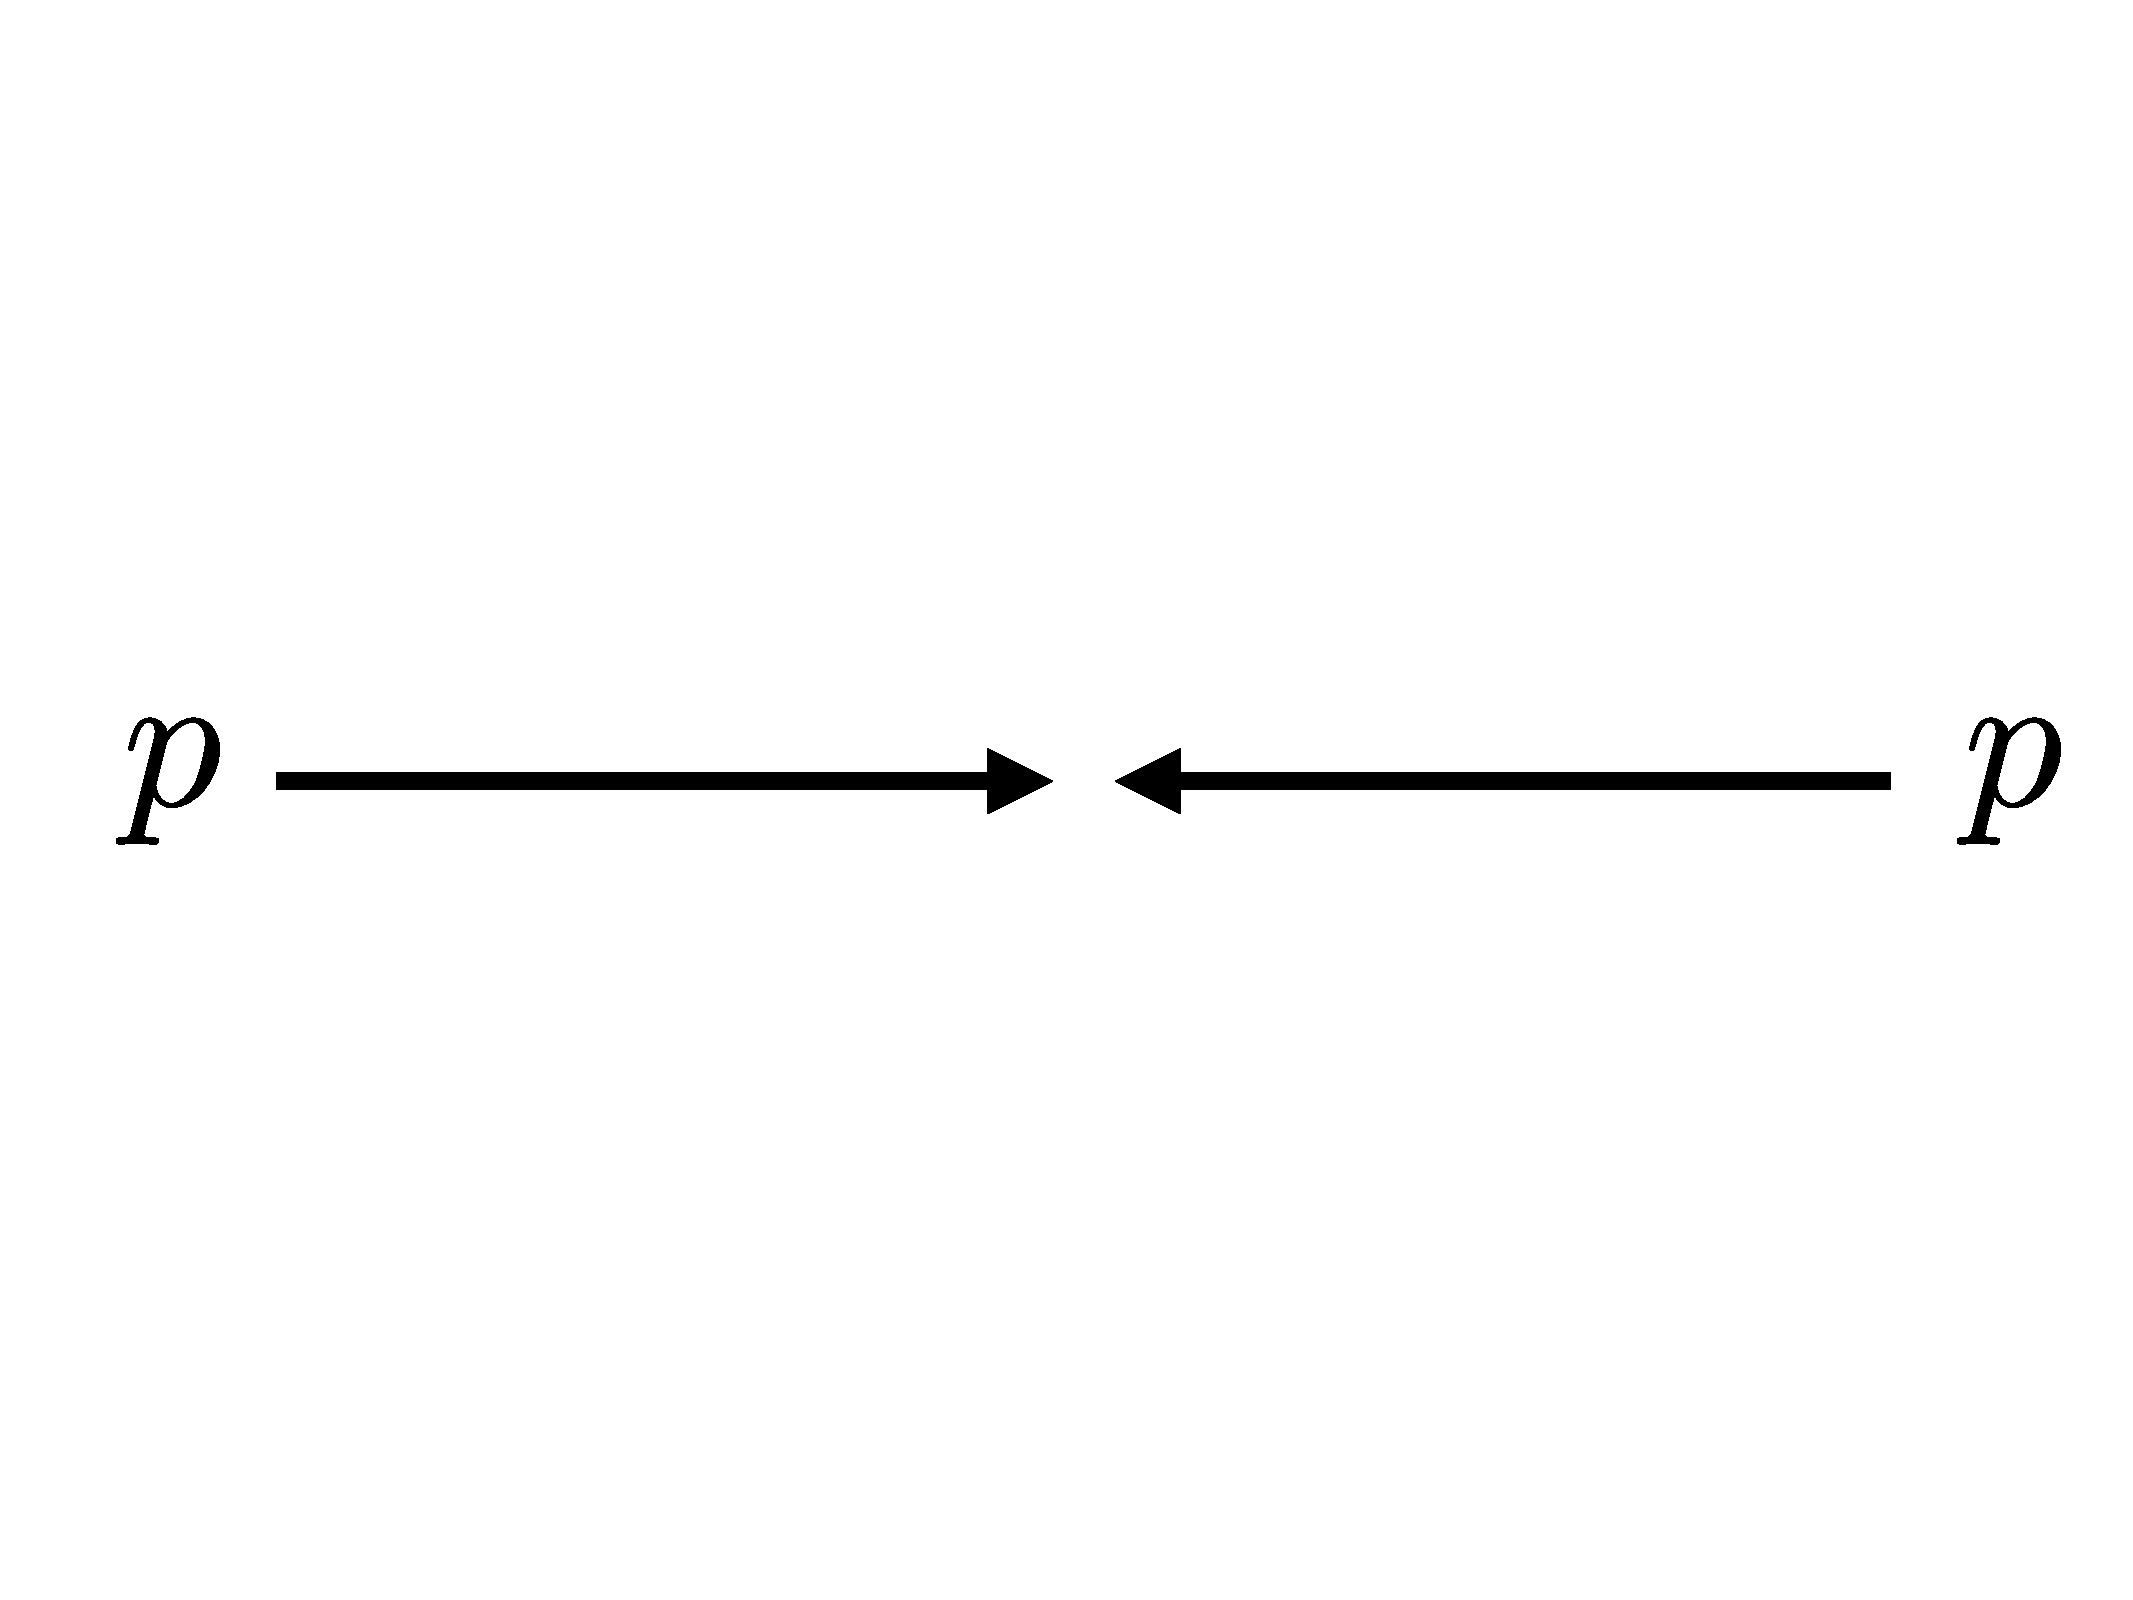
\includegraphics[scale=0.25]{stato_iniziale.pdf} 
\caption{Stato iniziale.} 
\end{figure}
Avremo quindi che
\newline


per il protone 1 avremo:
\begin{equation}
\textbf{P}_{1} = (E\> |\> 0, 0, +p) 
\end{equation}
\newline
mentre per il protone 2
\begin{equation}
\textbf{P}_{2} = (E\> |\> 0, 0, -p) 
\end{equation}



Introduciamo una ulteriore approssimazione osservando che dal momento che i protoni sono molto energetici (limite ultra-relativistico $\beta$ $\longrightarrow$ 1) la massa del singolo protone \'e trascurabile ($E_{protone}$ $\approx$ $p_{protone}$).
\newline
Per il protone 1 avremo:
\begin{equation}
\textbf{P}_{1} = (p\> |\> 0, 0, +p) 
\end{equation}
\newline
mentre per il protone 2
\begin{equation}
\textbf{P}_{2} = (p\> |\> 0, 0, -p) 
\end{equation}


Possiamo quindi scrivere: 
\newline

$\textbf{Stato iniziale}$: 
\begin{equation}
\textbf{P}_{in} = (p\> |\> 0, 0, p) + (p\> |\> 0, 0, -p) = (2p\> |\> 0, 0, 0)
\end{equation}

Calcoliamo la massa invariante del sistema $\sqrt{s}$ che per definizione non \'e altro che il modulo quadro del quadrivettore $\textbf{P}_{in}$, ossia:

\begin{equation}
s = \textbf{P}_{in} \cdot \textbf{P}_{in} = (2p)^2 = 4p^2
\end{equation}
\begin{figure}[h] 
\centering 
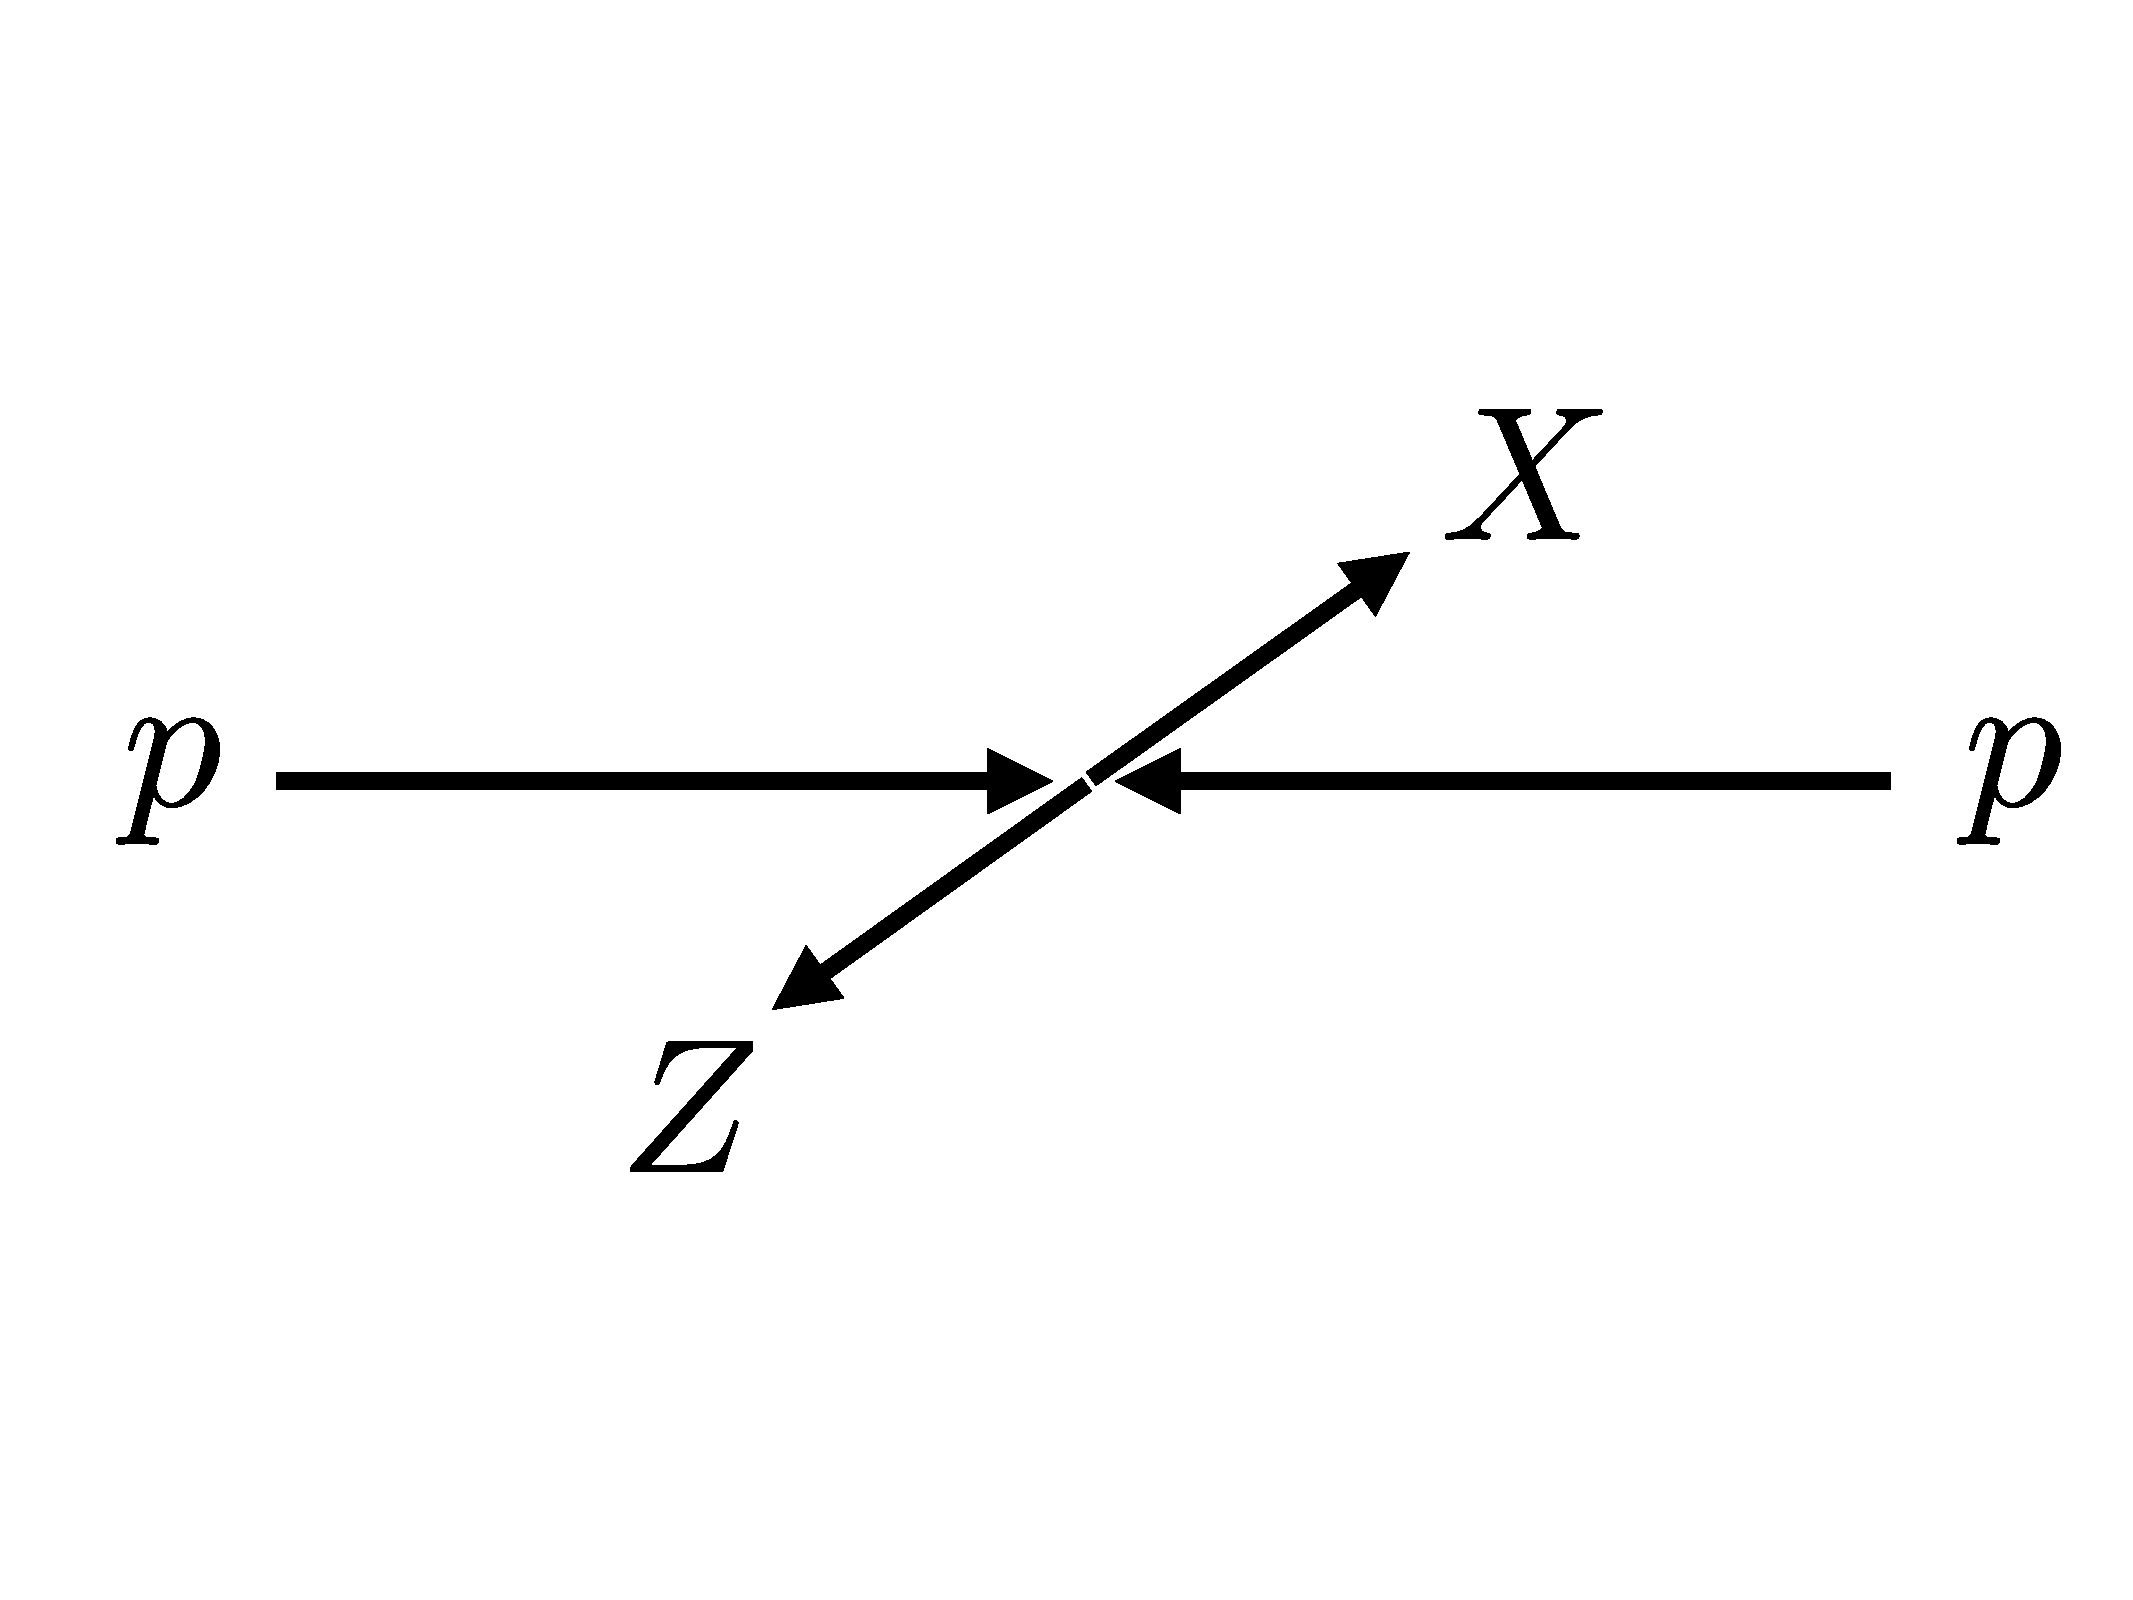
\includegraphics[scale=0.25]{stato_finale.pdf} 
\caption{Stato finale.} 
\end{figure}

Nello stato finale le componenti $z$ degli impulsi finali del primo e del secondo protone risulteranno variate
\begin{equation}
p_{z1} = p (1 - \xi_{1} )
\end{equation}
\begin{equation}
p_{z2} = p (1 - \xi_{2} )
\end{equation}


dove $\xi_{1}$ e $\xi_{2}$ sono definiti come $\xi_{1}$ $\equiv$ {$\Delta$$p_1$}/$p$, $\xi_{2}$ $\equiv$ {$\Delta$$p_2$}/$p$
\newline

Quindi i quadrivettori finali dei due protoni saranno:

\begin{equation}
\textbf{P $'$}_1 = (p\> |\> 0, 0, p (1 - \xi_{1} )) 
\end{equation}
\begin{equation}
\textbf{P $'$}_2 = (p\> |\> 0, 0, p (1 - \xi_{2} )) 
\end{equation}


$\textbf{Stato finale}$:
\begin{equation}
\textbf{P}_{fin} = (p(1 - \xi_1)\> |\> 0, 0, p(1 - \xi_1)) + (p(1 - \xi_2)\> |\> 0, 0, - p(1 - \xi_2)) + \textbf{P}_{XZ,LAB}
\end{equation}

Dove $P_{XZ,LAB}$ corrisponde al quadrimpulso del sistema formato dalla particella $X$ e $Z$ nel sistema del laboratorio. 
\newline

Applichiamo adesso il principio di conservazione del quadrimomento al sistema dei due protoni:
\begin{equation}
\textbf{P}_{in}  = \textbf{P}_{fin} \\
                             = (p(1 - \xi_1)\> |\> 0, 0, p(1 - \xi_1)) + (p(1 - \xi_2)\> |\> 0, 0, - p(1 - \xi_2)) + P_{XZ,LAB}
\end{equation}
\newline
Esplicitamente $P_{XZ,LAB}$ risulta essere

\begin{equation}
\textbf{P}_{XZ, LAB} = (p(\xi_1 + \xi_2) \> |\> 0, 0, p (\xi_2 - \xi_1)
\end{equation}


Calcoliamo la massa invariante del sistema $X$, $Z$ semplicemente applicando la definizione, ossia calcolando il modulo quadro del quadrimomento $P_{XZ, LAB}$

\begin{equation}
{{m}_{XZ}}^2 = {P_{XZ, LAB}}^2 = s \> \xi_1 \> \xi_2
\end{equation}
\newline

Spostiamoci adesso nel sistema di riferimento del centro di massa del sistema formato dalla particella $X$ e $Z$.

\begin{figure}[h] 
\centering 
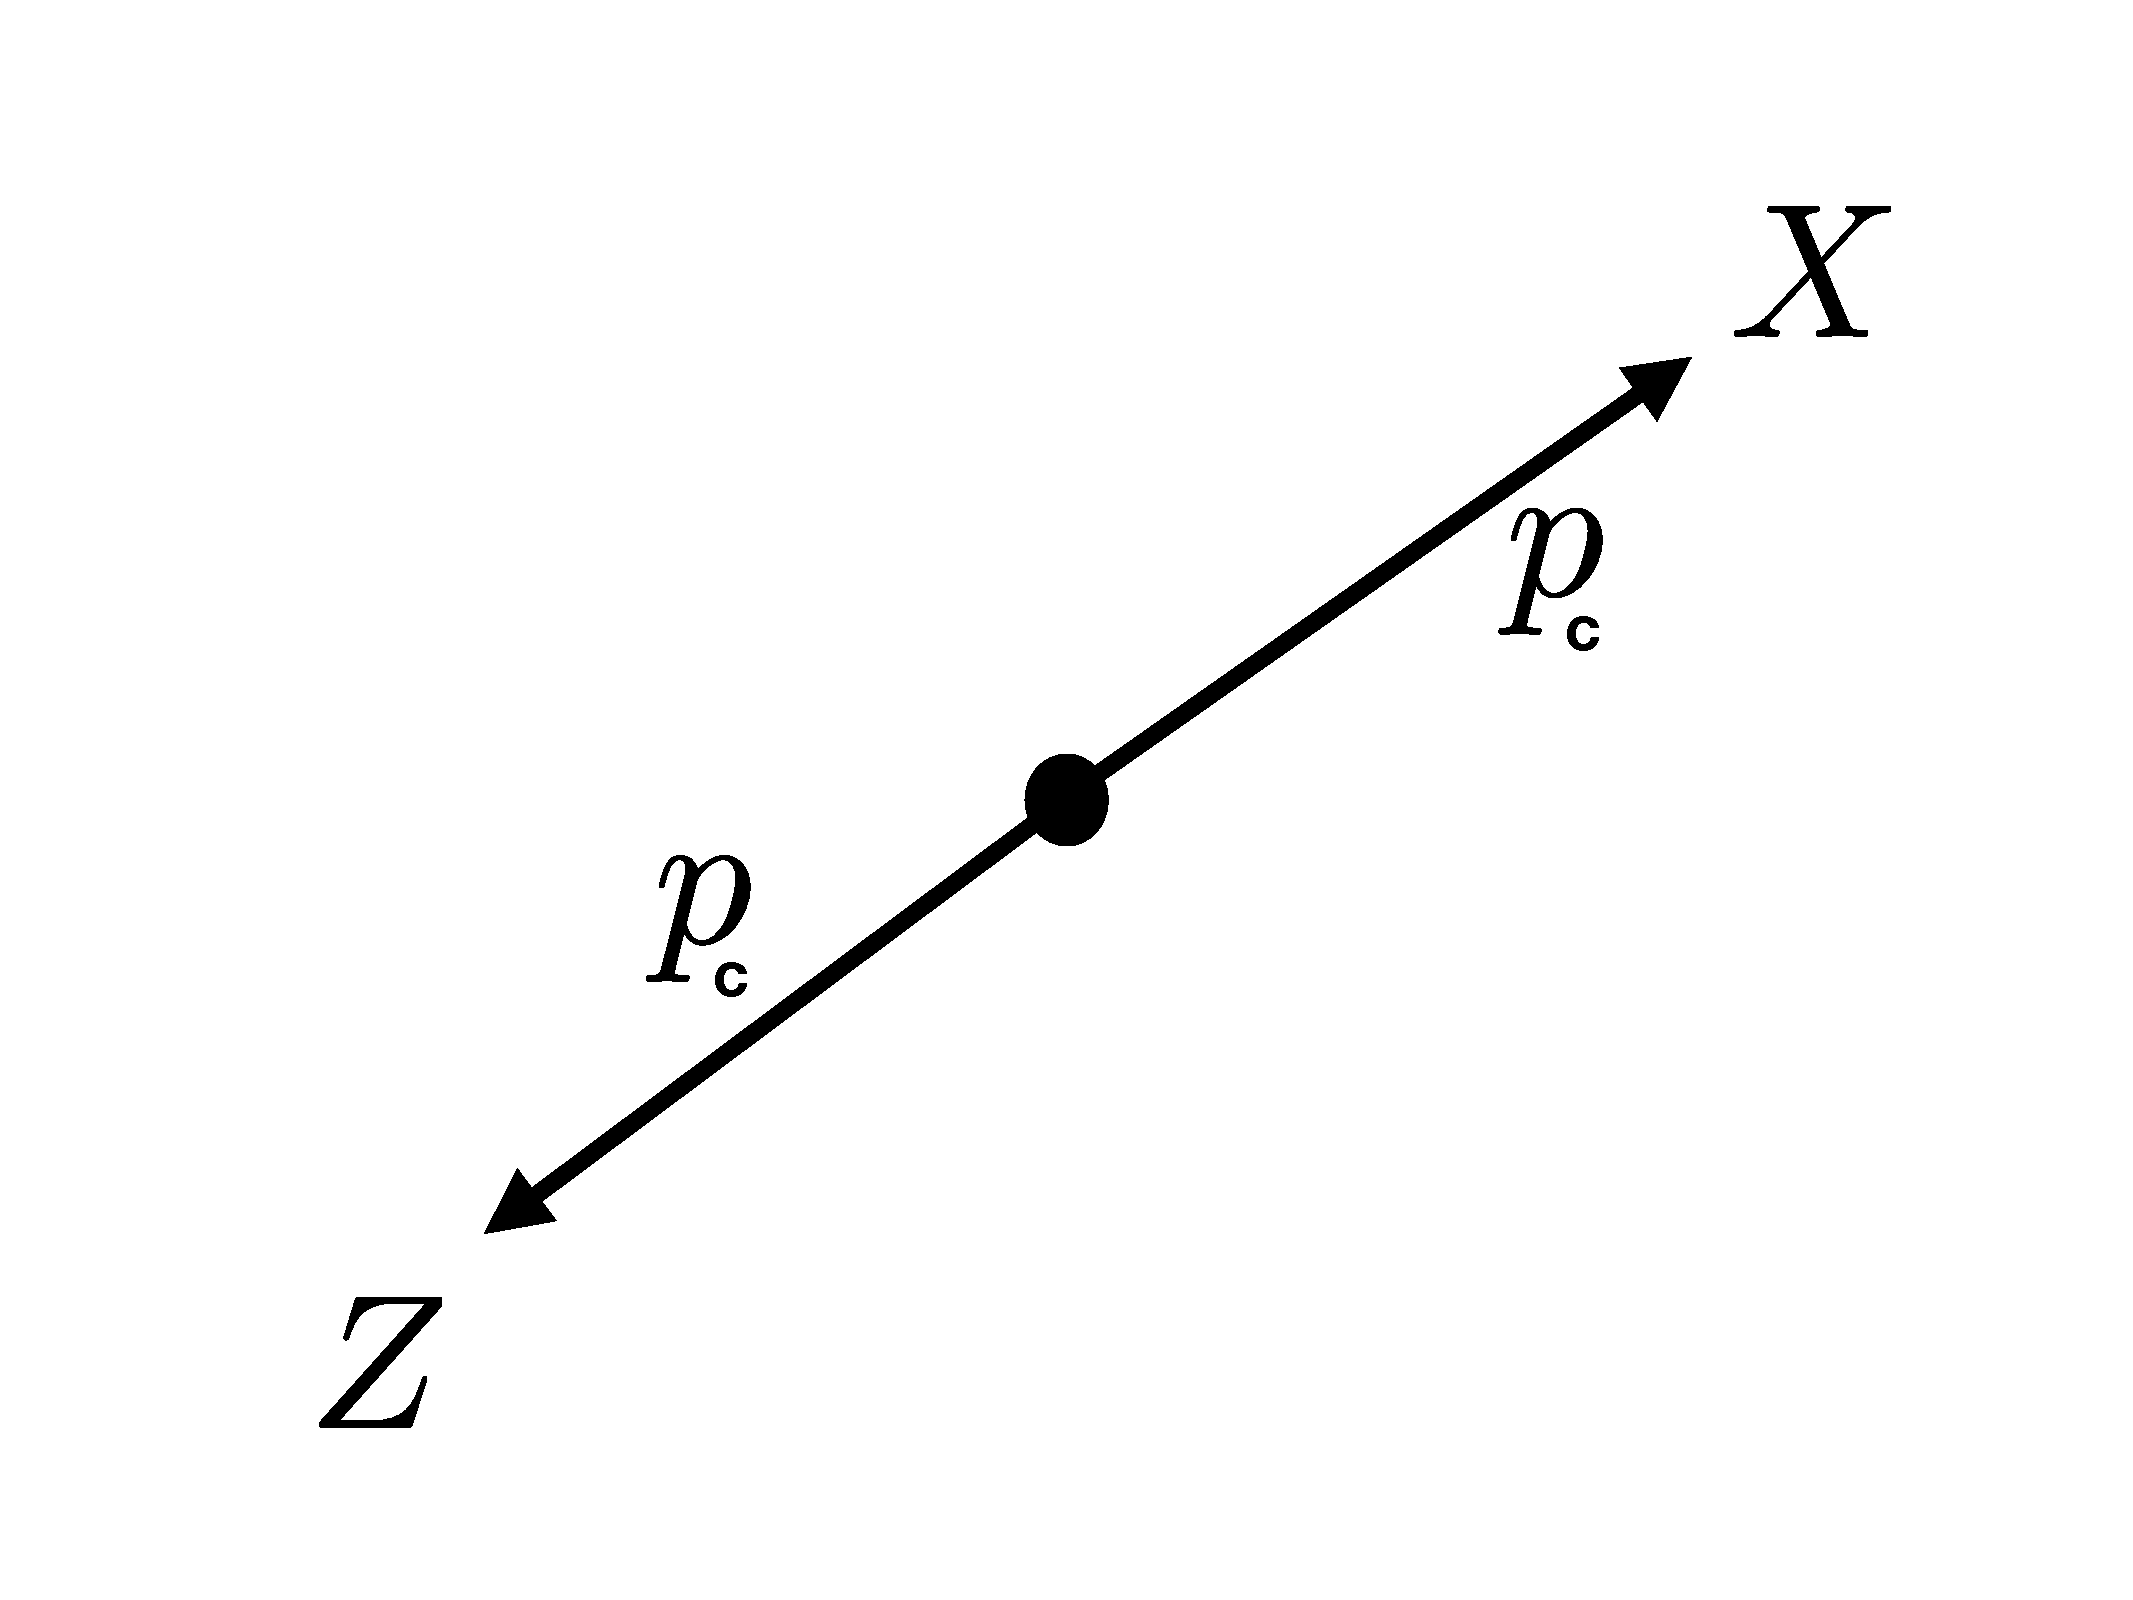
\includegraphics[scale=0.25]{cms_XZ.pdf} 
\caption{Sistema di riferimento del centro di massa del sistema XZ.} 
\end{figure}

Definiamo $p_c$ come l'impulso delle due particelle nel sistema del centro di massa, che scritto in notazione di quadrivettore risulta 

\begin{equation}
\textbf{P}_{XZ,CMS} = (E_X + E_Z \> |\> 0, 0, 0)
\end{equation}

Ovviamente soltanto la componente dell'energia risultare essere diversa da zero. Le altre componenti sono nulle per la definizione di impulso totale nel sistema di riferimento del centro di massa. 

Possiamo compattare la scrittura 
\begin{equation}
\textbf{P}_{XZ,CMS} = (E_{XZ, CMS} \> |\> 0, 0, 0)
\end{equation}

dove 
\begin{equation}
E_{XZ, CMS} = \sqrt{{m_X}^2 + {p_c}^2} + \sqrt{{m_Z}^2 + {p_c}^2}
\end{equation}

Sfruttiamo adesso il fatto che la massa invariante del sistema sia appunto un invariante relativistico e quindi avr\'a lo stesso valore sia prima che dopo l'interazione:

\begin{equation}
{\textbf{P}_{XZ, LAB}}^2 = {\textbf{P}_{XZ, CMS}}^2 
\end{equation}
\begin{equation}
 {m_{XZ}}^2 = {(\sqrt{{m_X}^2 + {p_c}^2} + \sqrt{{m_Z}^2 + {p_c}^2})}^2
\end{equation}

Elevando al quadrato ambo i membri e svolgendo alcuni passaggi algebrici \'e possibile ricavare l'espressione di $p_c$ in termini delle masse delle due particelle $m_X$, $m_Z$ e della massa invariante del sistema $m_{XZ}$

\begin{equation}
p_c = \sqrt{{1\over 4 {m_{XZ}}^2} ({m_{XZ}}^2 - {m_{X}}^2 - {m_{Z}}^2) - {{m_{X}}^2 {m_{Z}}^2 \over {m_{XZ}}^2}}
\end{equation}
\newline

Consideriamo adesso la componente dell'energia del quadrivettore 
\newline
$P_{XZ, LAB}$ = $p$($\xi_{1}$ + $\xi_{2}$). Adesso quello che faremo sar\'a scrivere tale componente nel sistema di riferimento del centro di massa (CMS) e per farlo utilizzeremo le trasformazioni di Lorentz.

\begin{equation}
\begin{pmatrix}
E_{XZ, LAB}\\
p_z '
\end{pmatrix}
 = \gamma
\begin{pmatrix}
1 & -\beta\\
-\beta & 1
\end{pmatrix}
\begin{pmatrix}
E_{XZ, CMS}\\
p_z 
\end{pmatrix}
\end{equation}



Prima abbiamo trovato che 

\begin{equation}
\textbf{P}_{XZ, LAB} = p\>(\xi_1 +\xi_2)
\end{equation}

applicando le trasformazioni di Lorentz 

\begin{equation}
\textbf{P}_{XZ, LAB} = \gamma \> (E_{XZ, CMS} - \beta \> P_{XZ, CMS})
\end{equation}
\newline
Come gi\'a visto precedentemente ${P}_{XZ, CMS}$ = 0 per definizione.
\newline

Mettiamo assieme i due risultati trovati:

\begin{equation}
p \> (\xi_1 + \xi_2) = \gamma \> (E_{XZ, CMS})
\end{equation}

dove $\gamma$ non \'e altro che il fattore di Lorentz

\begin{equation}
\gamma = {1 \over \sqrt{1 - {\beta}^2}}
\end{equation}
\newline
Quindi 

\begin{equation}
p \> (\xi_1 + \xi_2) = {1 \over \sqrt{1 - {\beta}^2}} \> E_{XZ, CMS} 
\end{equation}
\newline
dalla quale si pu\'o ricavare l'espressione di $\beta$ in funzione di $E_{XZ, CMS}$, di $p$ e di $\xi_1$, $\xi_2$
\begin{equation}
\beta = \sqrt{1 - {E_{XZ, CMS}\over p\>(\xi_1 +\xi_2)}}
\end{equation}
\newline

Tuttavia sorge un problema. Scritto $\beta$ in questa forma, esso ci dar\'a solo valori positivi e mai negativi (la radice quadrata di un numero \'e positivo o nullo per definizione). Per recuperare l'informazione sul segno di $\beta$ dobbiamo percorrere un'altra strada.

\begin{equation}
\textbf{P}_{XZ, LAB} = \mathcal{B}\>(\beta) \> \textbf{P}_{XZ, CMS}
\end{equation}
\newline
dove $\mathcal{B}\>(\beta)$ corrisponde alla matrice di Lorentz

\begin{equation}
\mathcal{B}\>(\beta)= \gamma\>\begin{pmatrix}
1 & \beta\\
-\beta & 1\end{pmatrix}
\end{equation}

Quindi, sostituendo avremo


\begin{equation}
\begin{pmatrix}
p \> (	\xi_1 + \xi_2)\\
p \> (	\xi_1 - \xi_2) \end{pmatrix}
 = \gamma \begin{pmatrix}
1 & \beta\\
-\beta & 1\end{pmatrix} 
\begin{pmatrix}
E_{XZ, CMS}\\
0 \end{pmatrix}
 = 
\begin{pmatrix}
\gamma\> E_{XZ, CMS}\\
\gamma\>(-\beta)\>E_{XZ, CMS} \end{pmatrix}
\end{equation}
\newline

Ricaviamo adesso l'espressione di $\beta$ dall'equazione seguente

\begin{equation}
{p \> (\xi_1 - \xi_2) \over p \>(\xi_1 + \xi_2)} = {\gamma \>(-\beta) \> E \over \gamma \>E} 
\end{equation}

che in definitiva, semplificando banalmente i termini uguali, porta ad avere
\newline

\begin{equation}
\beta = {\xi_2 - \xi_1 \over \xi_2 + \xi_1}
\end{equation}

risolvendo quindi il problema legato al segno di $\beta$\footnote{Infatti $\beta$ pu\'o essere sia positivo che negativo.}
\newline

Consideriamo adesso la particella $X$ nel sistema del centro di massa (CMS):

\begin{equation}
\vec{p}_X = \begin{pmatrix}
p_x\\
p_y\\
p_z \end{pmatrix}
 = p_c\>\begin{pmatrix}
\sin\theta\>\cos\varphi\\
\sin\theta\>\sin\varphi\\
\cos\theta\\
\end{pmatrix} 
\end{equation}
\newline

dove $\theta$ rappresenta l'angolo di scattering e avr\'a un valore random nell'intervallo (0, $\pi$), mentre $\varphi$ rappresenta l'angolo azimutale ed ha un valore random nell'intervallo (0, 2$\pi$).

Dato che ci siamo posti nel sistema del centro di massa, avremo che 
\begin{equation}
\vec{p}_Z = - \vec{p}_X
\end{equation}
\newline

Il quadrimpulso della particella $X$ nel CMS \'e
\begin{equation}
\textbf{P}_X = \begin{pmatrix}
\sqrt{{p_c}^2 + {m_X}^2}\\
p_c\>\sin\theta\>\cos\varphi\\
p_c\>\sin\theta\>\sin\varphi\\
p_c\>\cos\theta\\
\end{pmatrix} 
\end{equation}

analogamente per la particella $Z$, con l'unica differenza data dalla componente dell'energia del quadrimomento e il segno opposto per le restanti componenti:

\begin{equation}
\textbf{P}_Z = \begin{pmatrix}
\sqrt{{p_c}^2 + {m_Z}^2}\\
- p_c\>\sin\theta\>\cos\varphi\\
- p_c\>\sin\theta\>\sin\varphi\\
- p_c\>\cos\theta\\
\end{pmatrix} 
\end{equation}
\newpage

Per\'o a noi quello che interessa sono le espressioni dei quadrimomenti delle due particelle nel sistema di riferimento del laboratorio ($LAB$). Applichiamo semplicemente le trasformazioni di Lorentz del quadrimpulso

\begin{equation}
\begin{pmatrix}
 E_{XZ, LAB}\\
p_z  ' 
\end{pmatrix}
= 
\gamma \begin{pmatrix}
 E_{XZ, CMS} - \beta p_z\\
p_z - \beta E_{XZ, CMS}
\end{pmatrix} 
\end{equation}

Particella $X$ nel sistema di laboratorio:


\begin{equation}
\textbf{P}_X = \begin{pmatrix}
\gamma \sqrt{{p_c}^2 + {m_X}^2} - \gamma\> \beta\> p_c \cos\theta\\
 p_c\>\sin\theta\>\cos\varphi\\
 p_c\>\sin\theta\>\sin\varphi\\
\gamma\> p_c\cos\theta - \gamma \beta \sqrt{{p_c}^2 + {m_X}^2}\\
\end{pmatrix} 
\end{equation}


Particella $Z$ nel sistema di laboratorio:


\begin{equation}
\textbf{P}_Z = \begin{pmatrix}
\gamma \sqrt{{p_c}^2 + {m_Z}^2} - \gamma\> \beta\> p_c \cos\theta\\
 - p_c\>\sin\theta\>\cos\varphi\\
 - p_c\>\sin\theta\>\sin\varphi\\
\gamma\> p_c\cos\theta - \gamma \beta \sqrt{{p_c}^2 + {m_Z}^2}\\
\end{pmatrix} 
\end{equation}
\newline

Abbiamo quindi ricavato le espressioni dei quadrimpulsi delle due particelle. \newline
Queste, assieme al $\beta$, sono necessarie per poter ricavate le grandezze cinematiche di nostro interesse, e tali espressioni sono state implementate nel codice della macro di root.
Esse sono:
\begin{itemize}
\item momento trasverso $p_T$
\item componente $z$ del momento $p_z$
\item momento totale $p_{tot}$
\item angolo di scattering $\theta$
\item pseudo-rapidit\'a $\eta$
\end{itemize}

\subsection{Rapidit\'a e pseudorapidit\'a}
La rapidit\'a rappresenta una variabile utile da definire nello studio di uno scattering tra particelle in cui le reazioni sono del tipo $a$ + $b$ $\rightarrow$ $c$ + $d$, dove si \'e interessati soltanto alla particella prodotta $c$.
Analiticamente la rapidi\'a viene definita come 
\begin{equation}
y = {1 \over 2}\>log\>\Bigl(\>{{E + p_z }\over{E - p_z}}\>\Bigl)
\end{equation}

che nel limite non relativistico ($m$ $\gg$ $p$) viene approssimata a $y$ $\sim$ $v_z$.\newline

Nel passaggio ad un sistema di riferimento che si muove lungo $z$ rispetto a quello iniziale, la distribuzione di rapidit\'a non cambia forma. Il suo valore viene semplicemente traslato della quantit\'a:
\begin{equation}
y_0 = log\>|\>\gamma (\>1 + \beta \>)\>| .
\end{equation}
 
Mentre invece nel caso relativistico ($m$ $\ll$ $E$), la rapidit\'a si approssima alla pseudorapidit\'a:

\begin{equation}
\eta = - ln\>\Bigl[\>tan\>\Bigl(\>{\theta \over 2}\>\Bigl)\>\Bigl]
\end{equation}

Valgono inoltre le relazioni

\begin{equation}
p_z = m_T\> sinh\>y
\end{equation}
\begin{equation}
E = m_T\> cosh\>y
\end{equation}

dove
\begin{equation}
m_T = \sqrt{(\> {p_T}^2 + m^2 )}
\end{equation}


I rivelatori di CT-PPS rilevano particelle cariche solo in un certo intervallo limitato dell'angolo $\theta$ tra la traiettoria di una particella e l'asse del fascio ($z$).

Per angolo $\theta$ = 0 la pseudorapidit\'a \'e divergente $\eta$ = $\infty$ mentre $\eta$ = 0 per particelle perpendicolari all'asse del fascio ($\eta$ = $\pi$/2). La pseudorapidit\'a \'e usata spesso nella regione in avanti per distinguere tra particelle con angoli molto piccoli. 

%%%%%%%%%%%%%%%%%%%%%%%%%%%

\chapter{Software di simulazione e ricostruzione dei Roman Pot}
Come menzionato precedentemente uno degli scopi dell'esperimento CT-PPS \'e quello di misurare le variabili cinematiche dei protoni scatterati a seguito di un'interazione nell'intervallo pi\'u ampio possibile - in particolare i pi\'u importanti sono il trasferimento di quantit\'a di moto $t$ (o angolo di scattering equivalente ${\theta}^{*}$) e la perdita frazionaria di momento $\xi$ dei protoni diffrattivamente dispersi all'IP.
La corrispondente distribuzione di queste variabili rappresenta un importante input sperimentale necessario per alcuni ulteriori studi teorici sulle interazioni tra protoni e sulla loro struttura.
 \newline
 
 Ad ogni modo il programma da me sviluppato non \'e finalizzato ad ottenere le distribuzioni delle variabili cinematiche dei protoni, bens\'i quelle delle due particelle prodotte dalle interazioni (particelle $Z$, $X$), come discusso nell'ultimo paragrafo del Capitolo 3.
 Il motivo di tutto ci\'o sta nel fatto che il nostro obiettivo consiste nel simulare uno scattering tra protoni in cui una delle due particelle prodotte, in questo caso la $X$ \'e del tutto sconosciuta e quindi, attribuendole differenti valori di massa (nel nostro caso, $m_X$ = 800 GeV, 1000 GeV,1200 GeV, 1400 GeV, 1600 GeV) sar\'a possibile confrontare i risultati delle diverse simulazioni con i dati sperimentali ottenuti durante l'anno 2017.
 
 Per poter simulare le distribuzioni delle variabili cinematiche (momento trasverso $p_T$, componente $z$ del momento $p_z$, momento totale $p_{tot}$, angolo di scattering $\theta$, pseudo-rapidit\'a $\eta$) sia della $Z$, che della $X$, \'e stata scritta una macro di Root chiamata \texttt{LorenzoGenerator.cc}.
Tuttavia il mio lavoro non si esaurisce qui. Infatti \texttt{LorenzoGenerator.cc} non solo fornisce importanti informazioni sulla cinematica delle due particelle prodotte, ma anche i valori di $t$ e $\xi$ dei protoni scatterati.
Successivamente questi valori sono passati ad altri due programmi, chiamati \texttt{test$\_$gen$\_$simu$\_$cfg.py} e \texttt{test$\_$gen$\_$simu$\_$smear$\_$cfg.py}, il cui compito consiste nel rappresentare la distribuzione spaziale dei protoni rilevati dai Roman Pot, sia a destra che a sinistra dell'IP.
 La differenza sostanziale tra i due programmi sta nel semplice fatto che mentre \texttt{test$\_$gen$\_$simu$\_$cfg.py} tiene conto del fenomeno di smearing solamente lungo la direzione del fascio, ossia l'asse $z$ (smearing lungo gli assi $x$ e $y$ nulli), \texttt{test$\_$gen$\_$simu$\_$smear$\_$cfg.py} tiene conto dello smearing anche lungo gli assi $x$ e $y$.
Risulta ovvio che \texttt{test$\_$gen$\_$simu$\_$smear$\_$cfg.py} costituisca una rappresentazione pi\'u fedele della realt\'a rispetto a \texttt{test$\_$gen$\_$simu$\_$cfg.py} il cui scopo ha un fine puramente didattico, ossia mettere in mostra i differenti risultati ottenuti nel caso in cui si considerino o meno i fenomeni di smearing.\newline

Il motivo di tutto ci\'o sta nel fatto che una buona comprensione dei processi che i protoni scatterati subiscono fino a quando non vengono rilevati dai rivelatori RP \'e essenziale per lo sviluppo e la messa a punto delle tecniche di ricostruzione (tecniche in cui la cinematica dei protoni sparsi viene dedotta dalle misurazioni RP). A tale scopo la simulazione Monte Carlo (MC) fornisce uno strumento molto prezioso.
 
\subsection{Software di simulazione}
In questo paragrafo verranno presentati soltanto gli aspetti salienti del codice che costituisce la macro di Root, ossia i punti che necessitano di pi\'u attenzione. Ad ogni modo, l'intero codice \'e consultabile nella branch di CMSSW\newline (\texttt{https://github.com/CTPPS/cmssw/tree/lorenzo\_generator}). 
In particolare il codice si trova all'indirizzo: \texttt{https://github.com/CTPPS/cmssw/blob/lorenzo\_generator}\newline\texttt{/Lorenzo/Test/src/LorenzoGenerator.cc}. A seguire vi \'e una breve descrizione dei componenti di \texttt{LorenzoGenerator.cc}:\newline
\begin{itemize}
\item  \textbf{Generatore di eventi}: Il processo di simulazione inizia con la generazione di particelle nel punto di interazione. Questo pu� essere una $particle$ $guns$" o un $physics$ $event$ $generator$". Le "$particle$ $guns$" generano particelle in base a determinate distribuzioni prestabilite. I generatori di eventi fisici costruiscono eventi in base a modelli fisici.
In \texttt{LorenzoGenerator.cc} lo scopo del generatore consiste nel generare l'evento di nostro interesse, ossia l'interazione tra due protoni in quello che abbiamo chiamato IP ($interation$ $point$). In particolare il generatore avr\'a una duplice funzione: da un lato creer\'a dei protoni scatterati che avranno perso un certo valore del loro momento iniziale e che saranno rilevati in un secondo momento dai RP, dall'altro creer\'a le due particelle $Z$ e $X$, le quali saranno invece rilevate dai rivelatori di CMS.
\item \textbf{Propagazione}: in questa parte viene simulata la traiettoria che il protone scatterato percorre all'interno dei magneti di LHC.
\item  \textbf{Simulazione dei RP}: in questa fase il software simula gli $hits$ rilevati dai Roman Pot, cio\'e le distribuzioni spaziali dei protoni scatterati che hanno raggiunto i rivelatori. 
\item  \textbf{Modulo di smearing}: l'obiettivo del modulo di smearing deve tenere conto degli effetti di smearing del fascio che di solito non sono considerati dai generatori di eventi. Questi effetti di smearing possono essere suddivisi in tre classi: smearing angolare (le particelle all'interno di un pacchetto non sono tutte parallele), smearing di energia (esiste una fluttuazione di energia all'interno di un pacchetto) e smearing dei vertici (le particelle hanno dimensione diversa da zero, quindi le interazioni sono distribuite nello spazio).
\end{itemize}

\begin{figure}[h!] 
\centering 
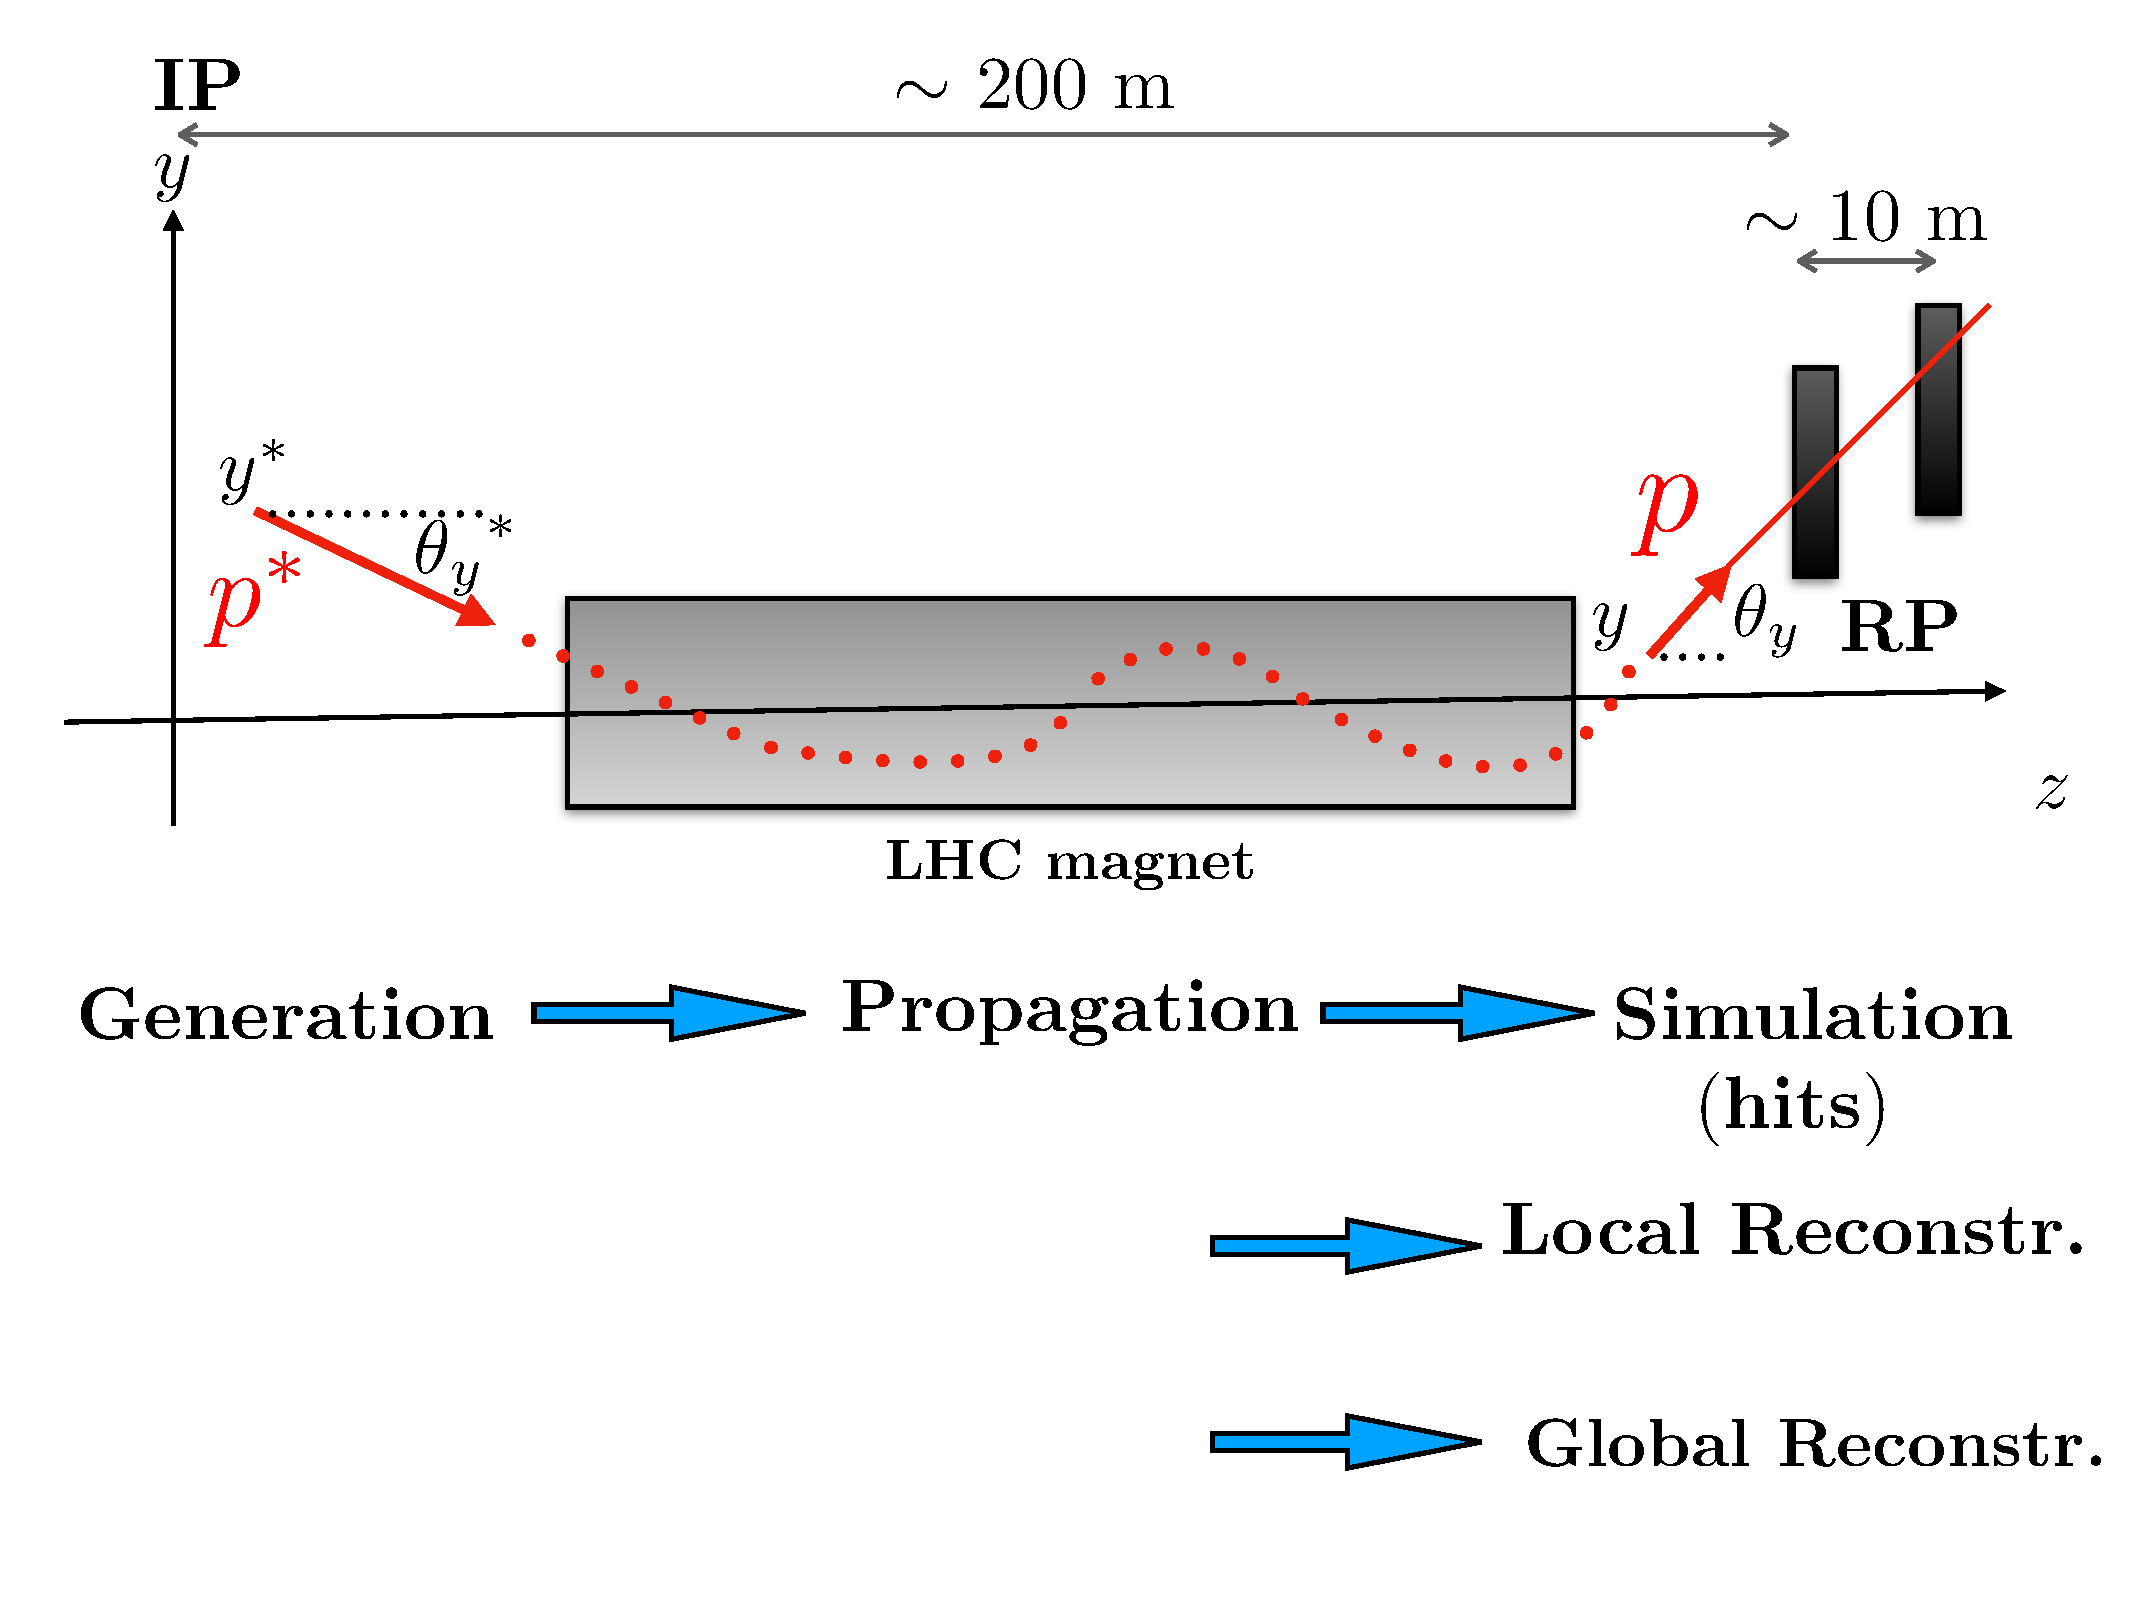
\includegraphics[scale=0.45]{schema_codice.pdf} 
\caption{Rappresentazione schematica delle diverse fasi del software \texttt{LorenzoGenerator.cc}. Dalla fase iniziale in cui viene generato l'evento di interazione tra i protoni si passa alla loro propagazione all'interno dei magneti di LHC. In fine si esegue la simulazione degli hits, ossia viene simulata la distribuzione spaziale dei protoni scatterati sui RP.} 
\end{figure}

L'importanza di tutto ci\'o risiede nel fatto che attraverso una ricostruzione locale delle tracce protoniche nei RP \'e possibile ricostruire globalmente l'evento fisico, in particolare ai valori di $\xi$ e $|t|$ all'IP.

Vediamo adesso pi\'u nel dettaglio, ma sempre da un punto di vista qualitativo, gli effetti dello smearing del fascio. Una trattazione pi\'u approfondita \'e consultabile in [7].


\subsection{Smearing angolare e di energia}
La maggior parte dei generatori di eventi descrive le collisioni in un sistema di riferimento (sistema di riferimento del centro di massa), dove le particelle incidenti si avvicinano l'un l'altra lungo l'asse $z$, ciascuna con il proprio momento nominale $p_{nom}$. Tuttavia, una vera collisione nel sistema del laboratorio sembra diversa, come \'e mostrato in Figura 4.1. A causa dello smearing dell'energia ogni protone incidente ha un momento leggermente diverso (di cui si tiene conto introducendo i fattori $\xi_1$ e $\xi_2$) e a causa dell'angolo di incrocio ($crossing$ $angle$) $\alpha$ e dello smearing angolare (i fattori $C_1$ e $C_2$) non si scontrano perfettamente frontalmente. Una parte di questi effetti di smearing pu� essere descritta da una trasformazione di Lorentz dal sistema del CM al sistema del LAB [7].

\begin{figure}[h!] 
\centering 
\includegraphics[scale=0.4]{energy_smear.pdf} 
\caption{Una collisione vista nel piano $xz$ nel sistema LAB. La quantit\'a di moto dei protoni viene alterata a causa dello smearing di energia, le direzioni sono modificate a causa dell'angolo di incrocio $\alpha$ e dello smearing angolare.} 
\end{figure}


\begin{figure}[h] 
\centering 
\includegraphics[scale=0.3]{vertex_smear.pdf} 
\caption{Una collisione tra due pacchetti sotto un $crossing$ $angle$ $\alpha$, descritto nel sistema del LAB.} 
\end{figure}

\newpage
\section{Istogrammi}
\subsection{Particella $X$}

Nel Capitolo 3 abbiamo studiato la cinematica dell'urto tra due protoni. Da questa analisi abbiamo infine ricavato le espressioni dei quadrimpulsi delle due particelle. \newline
Queste, assieme al $\beta$, sono necessarie per poter ricavate le grandezze cinematiche di nostro interesse le cui espressioni sono state implementate nel codice di \texttt{LorenzoGenerator.cc}.
Esse sono:
\begin{itemize}
\item momento trasverso $p_T$ 
\item componente $z$ del momento $p_z$
\item momento totale $p_{tot}$
\item angolo di scattering $\theta$
\item pseudo-rapidit\'a $\eta$
\end{itemize}
Di seguito \'e riportato il risultato della simulazione di \texttt{LorenzoGenerator.cc}, ovvero le  distribuzioni di frequenza di ciascuna delle grandezze, in questo caso della particella $X$, alla quale \'e stata attribuita una massa di valore casuale e arbitrario $m_X$ = 1.2 TeV.
   

\begin{figure}[h] 
\centering 
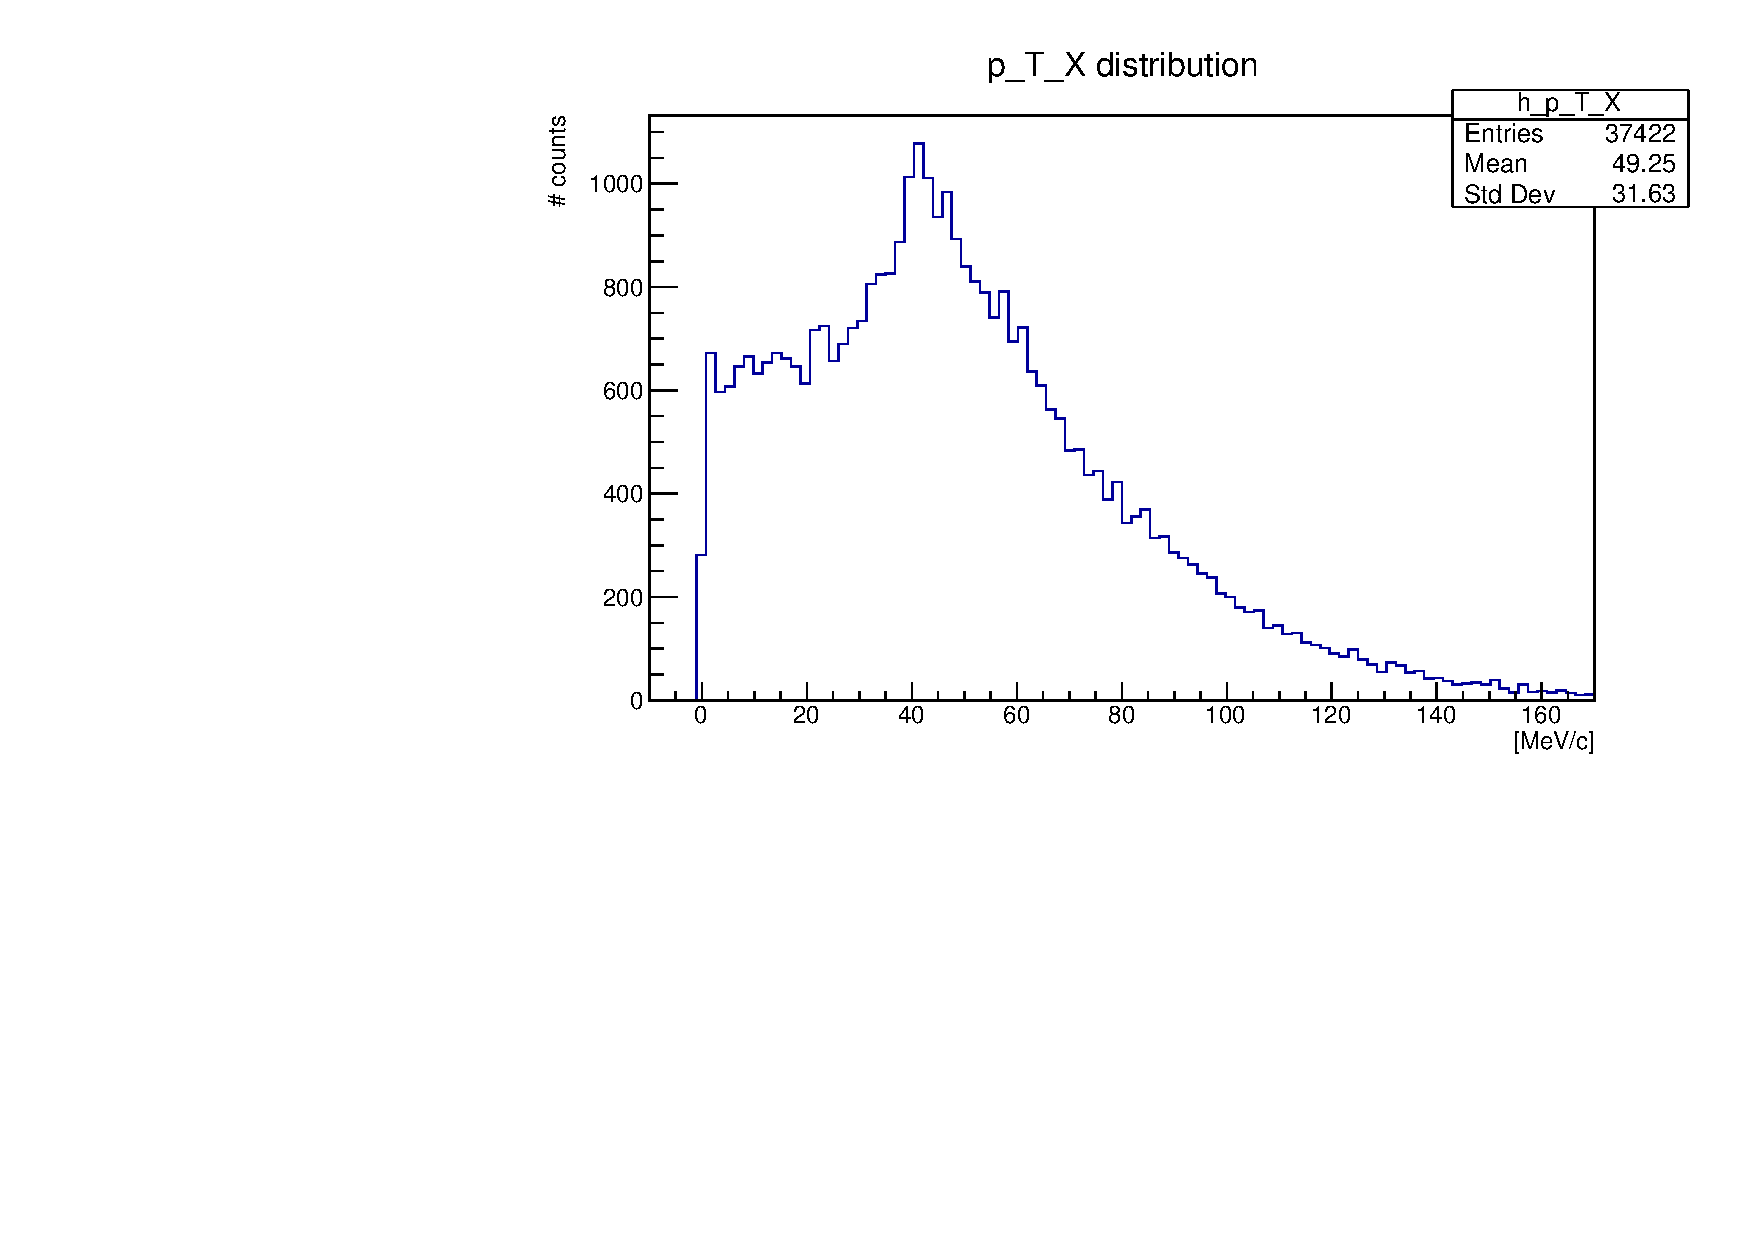
\includegraphics[scale=0.7]{p_T_X.pdf} 
\caption{Impulso trasverso della $X$.} 
\end{figure}

\begin{figure}[h] 
\centering 
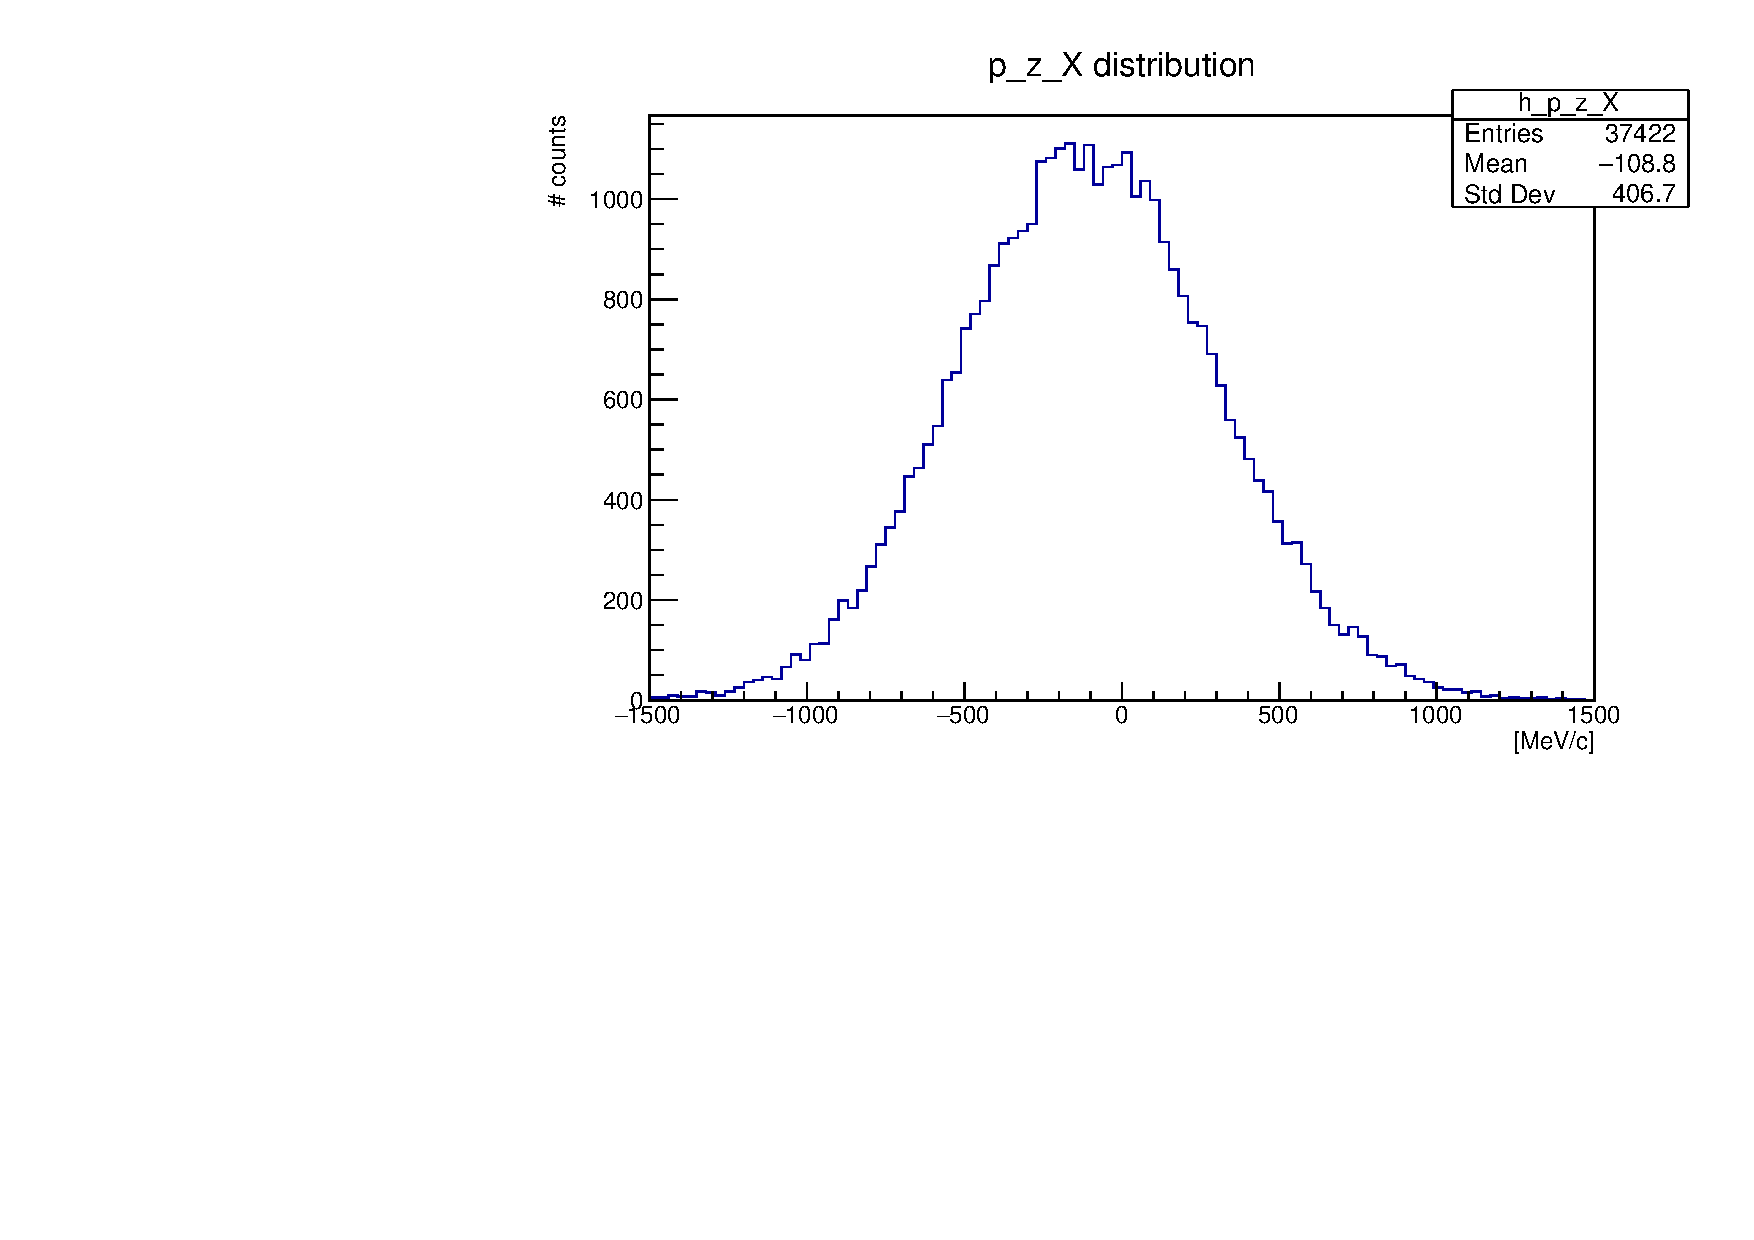
\includegraphics[scale=0.7]{p_z_X.pdf} 
\caption{Componente $z$ dell'impulso della $X$.} 
\end{figure}

\begin{figure}[h] 
\centering 
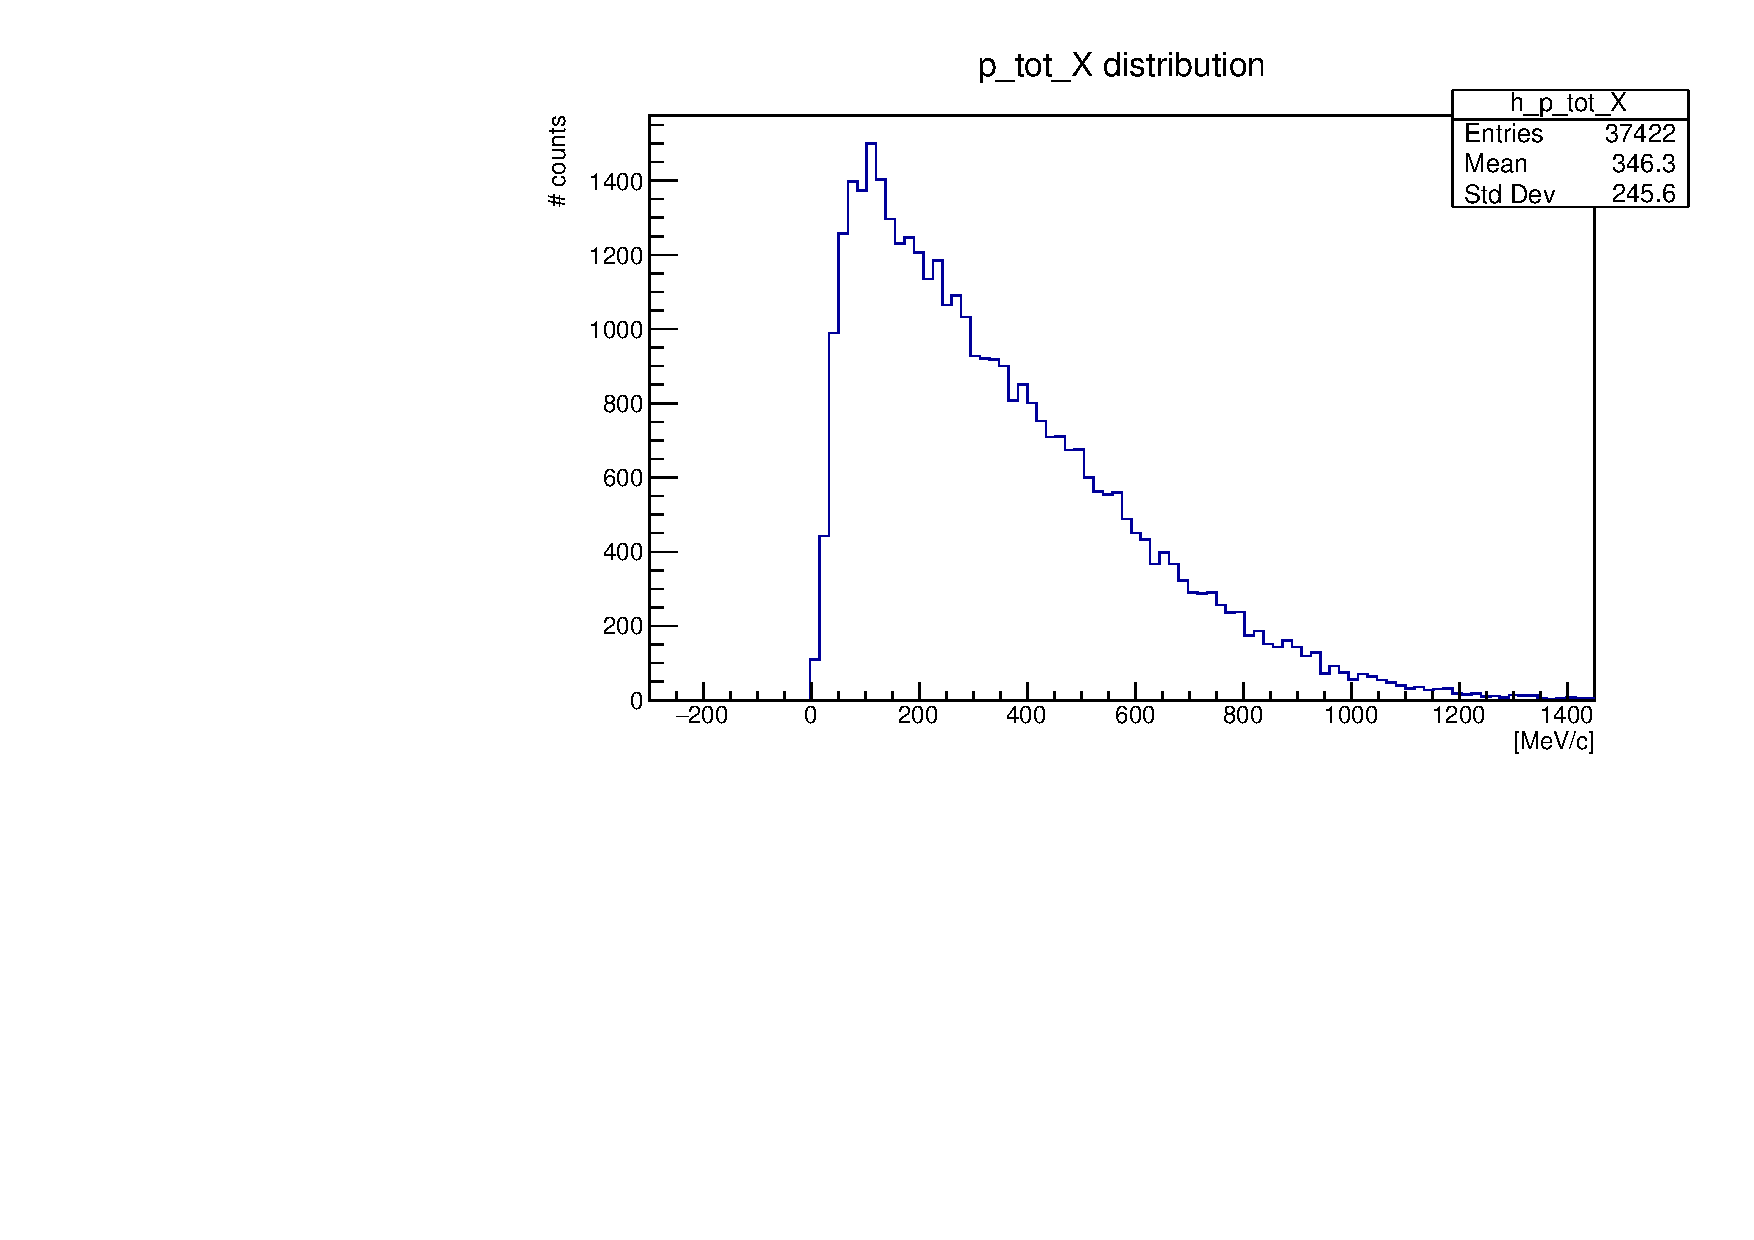
\includegraphics[scale=0.7]{p_tot_X.pdf} 
\caption{Impulso totale della $X$.} 
\end{figure}

\begin{figure}[h] 
\centering 
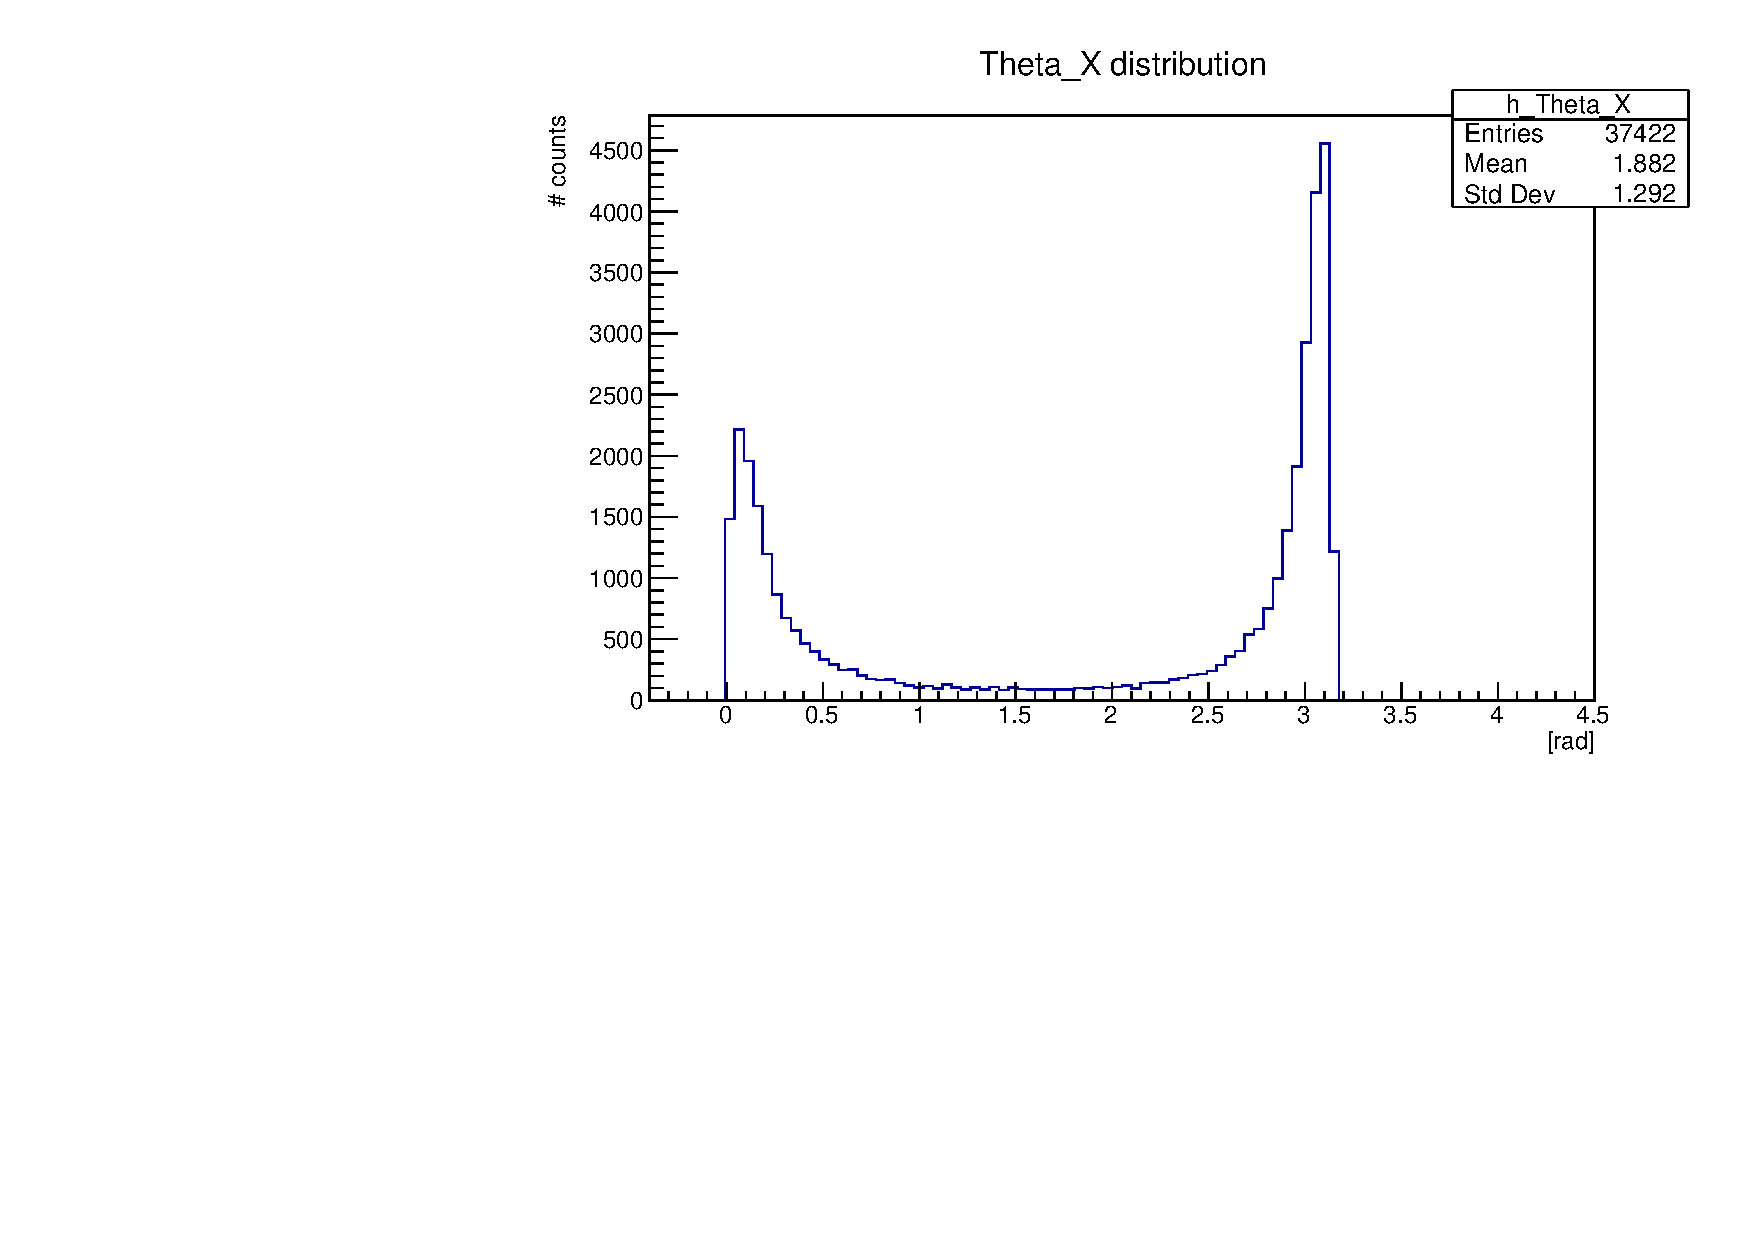
\includegraphics[scale=0.7]{Theta_X.pdf} 
\caption{Angolo $\theta$ della $X$.} 
\end{figure}

\begin{figure}[h] 
\centering 
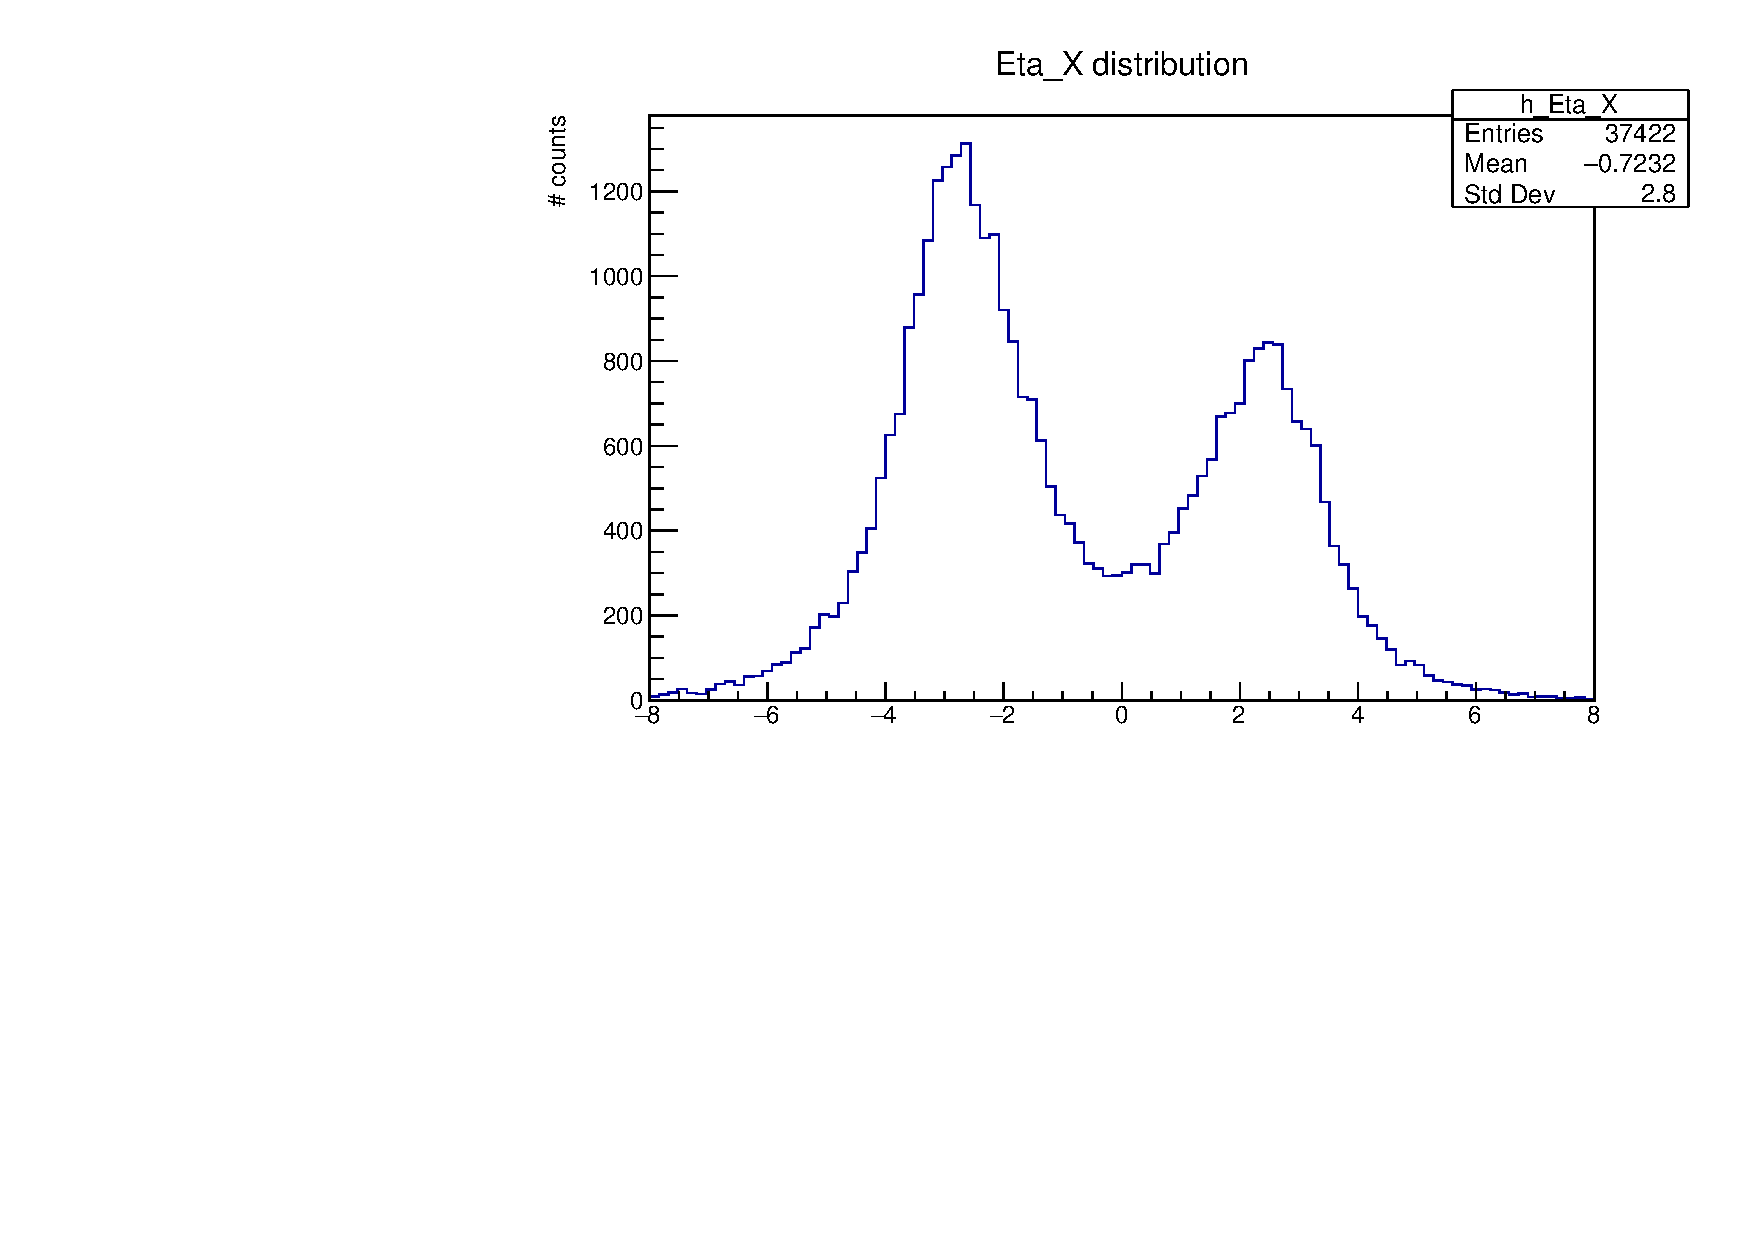
\includegraphics[scale=0.7]{Eta_X.pdf} 
\caption{Pseudo-rapidit\'a della $X$.} 
\end{figure}
\clearpage
\subsection{Particella $Z$}


La stessa procedura di analisi \'e stata fatta per la particella $Z$. Come spiegato precedentemente, la $Z$ che si origina dall'interazione tra i protoni rappresenta il bosone di gauge mediatore dell'interazione debole. Essa ha massa $m_{Z}$ = 91.1876 $\pm$ 0.0021 GeV/$c^2$, carica elettrica: 0 $e$, spin 1. Quindi in questo caso le caratteristiche sono note a priori.\newline

Le figure seguenti mostrano le distribuzioni di frequenza delle grandezze cinematiche studiate, le quali sono state successivamente affiancate a quelle della particella $X$ per enfatizzarne le differenze.

\begin{figure}[h] 
\centering 
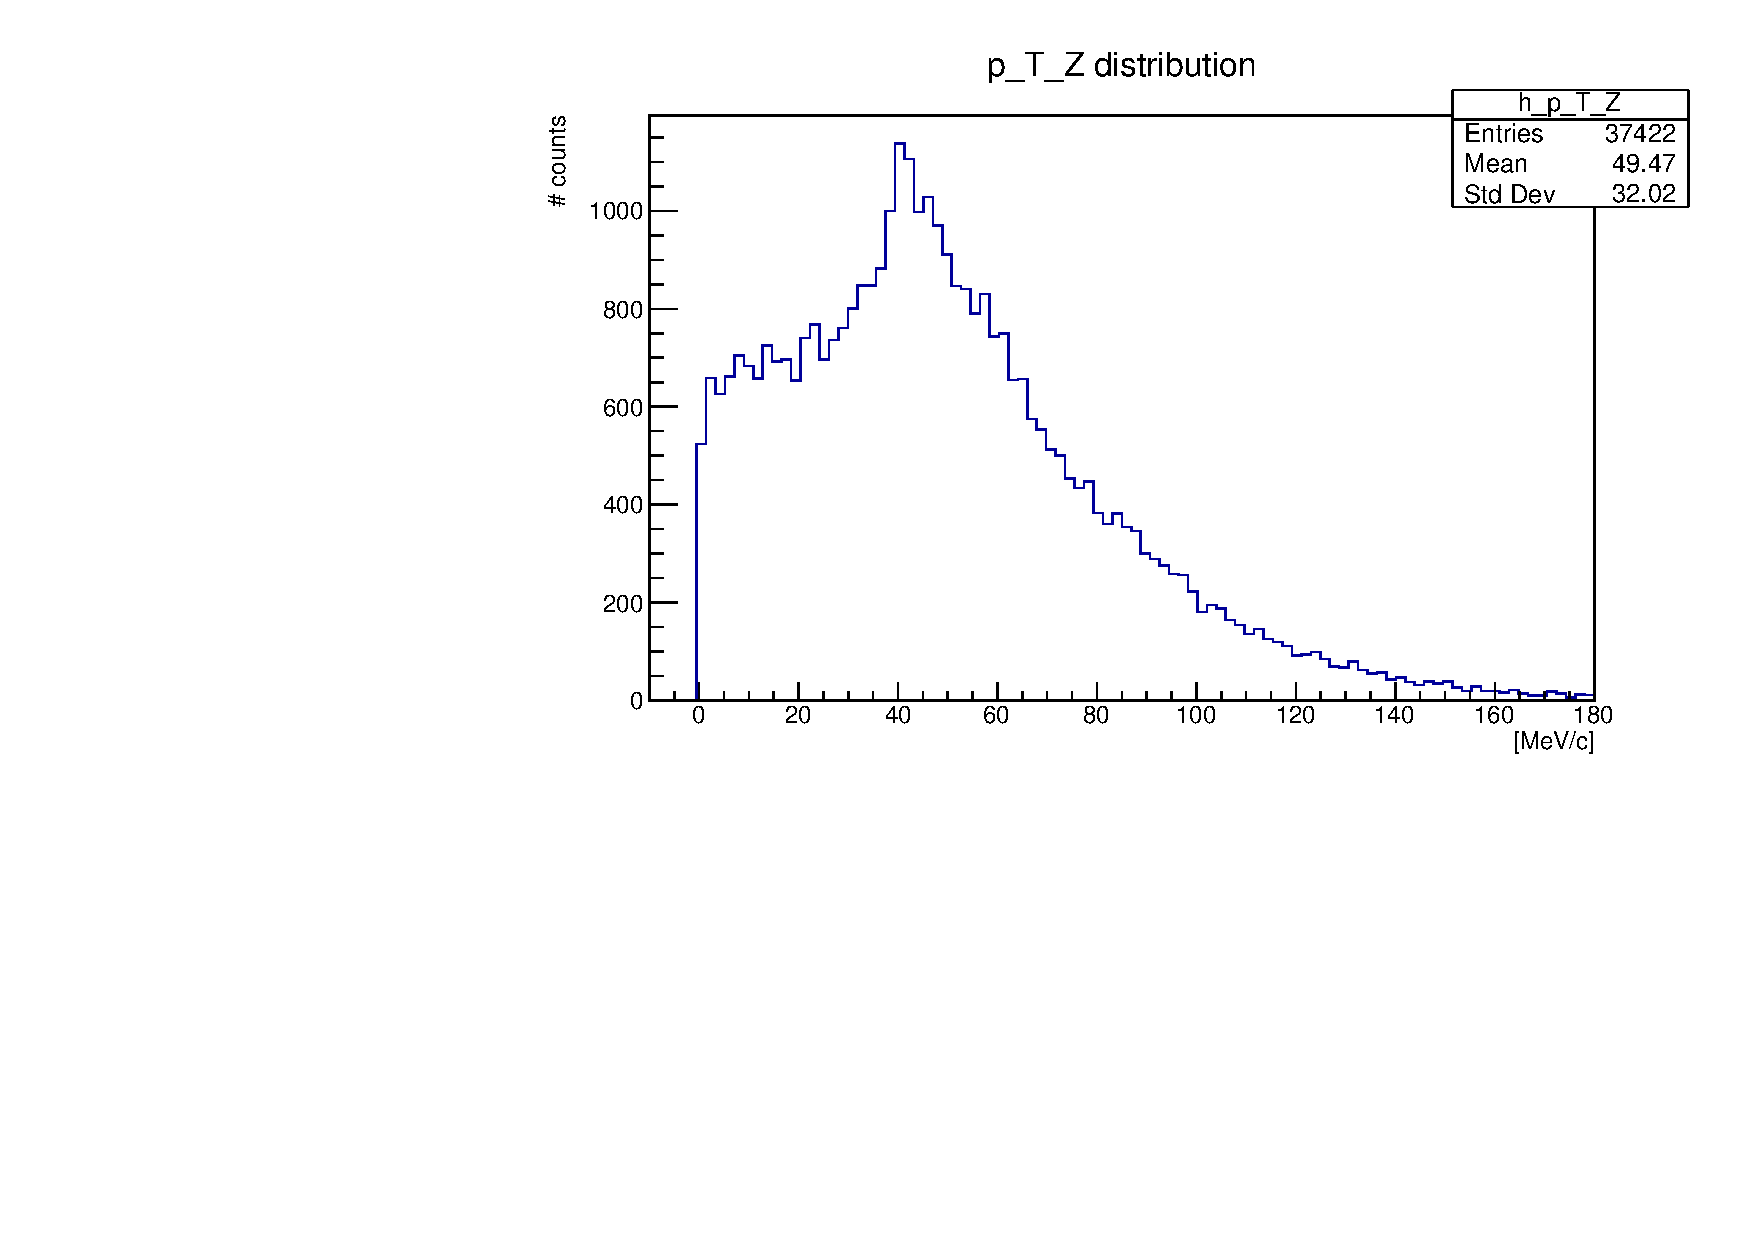
\includegraphics[scale=0.7]{p_T_Z.pdf} 
\caption{Impulso trasverso della $Z$.} 
\end{figure}

\begin{figure}[h] 
\centering 
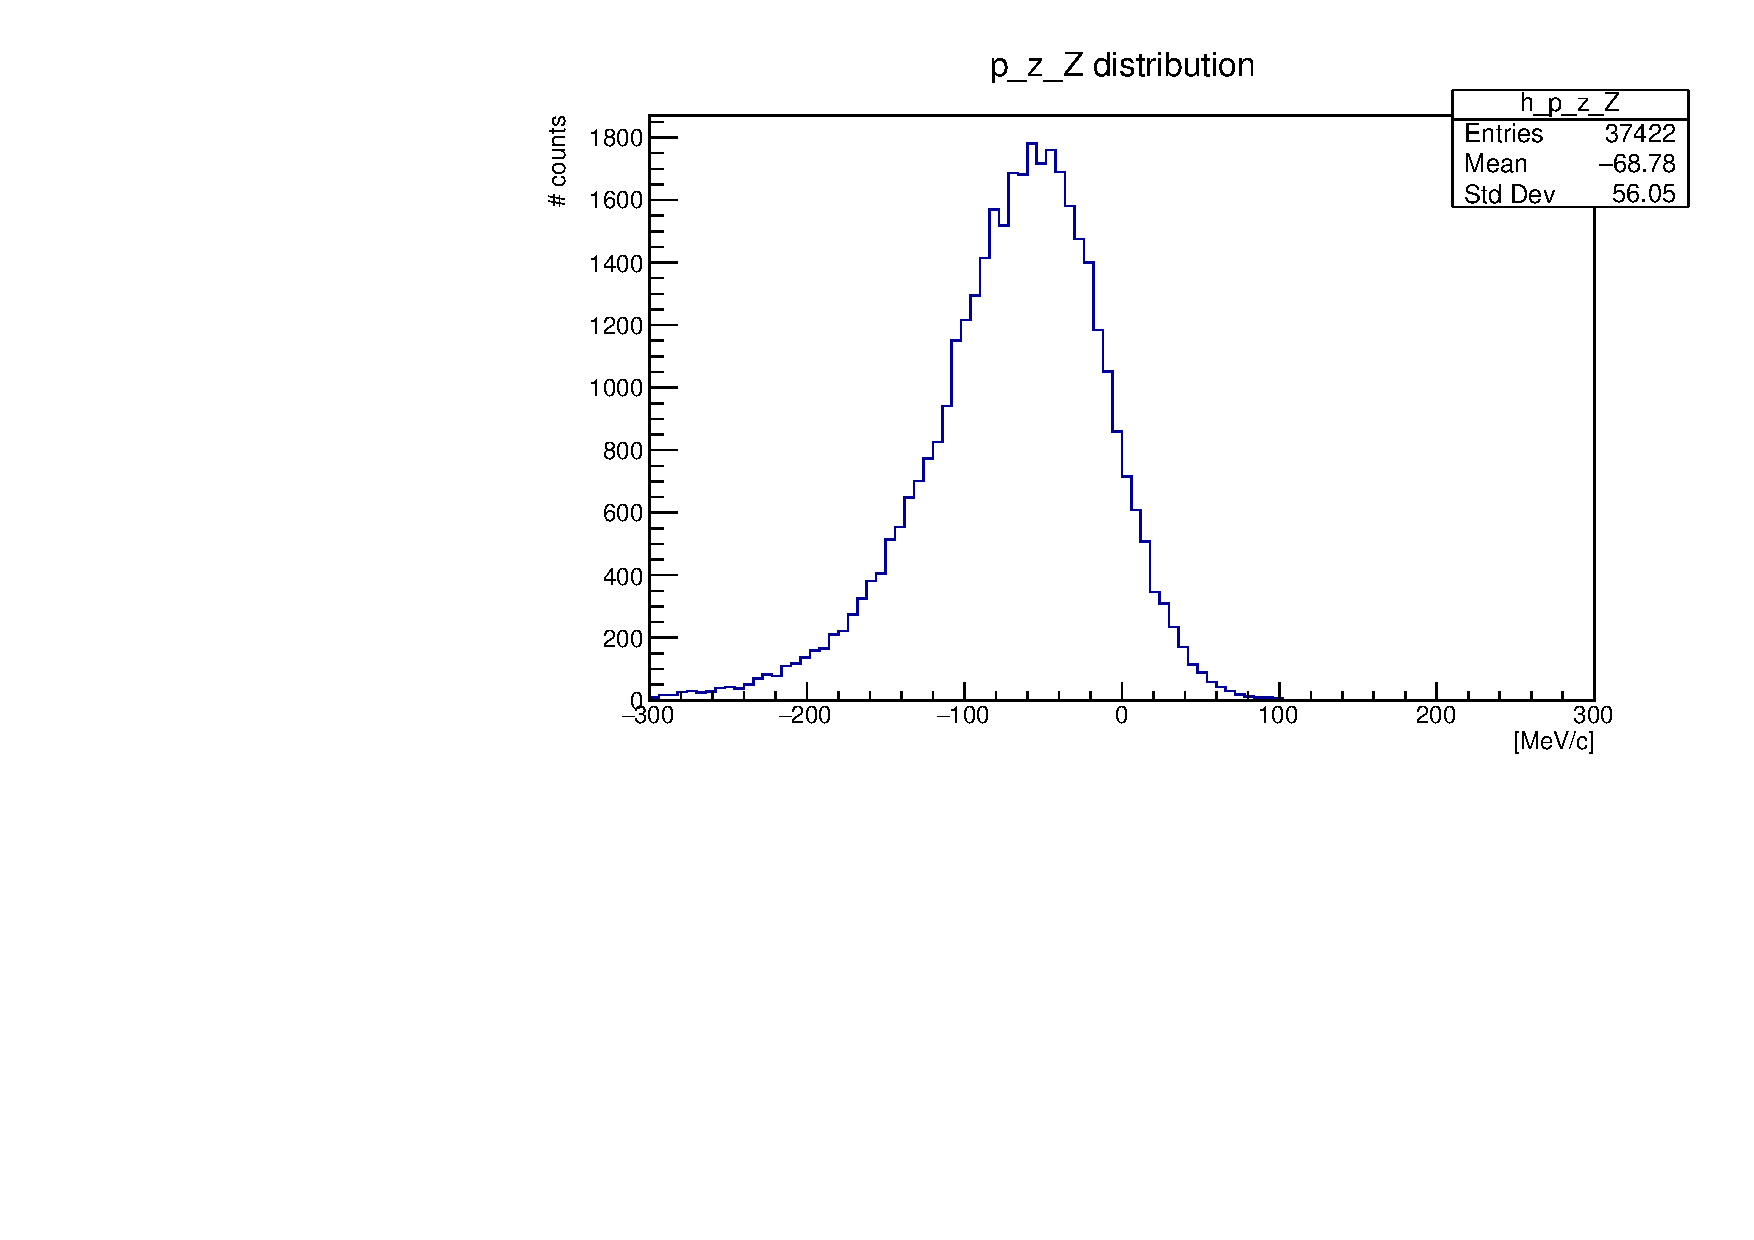
\includegraphics[scale=0.7]{p_z_Z.pdf} 
\caption{Componente $z$ dell'impulso della $Z$.} 
\end{figure}

\begin{figure}[h] 
\centering 
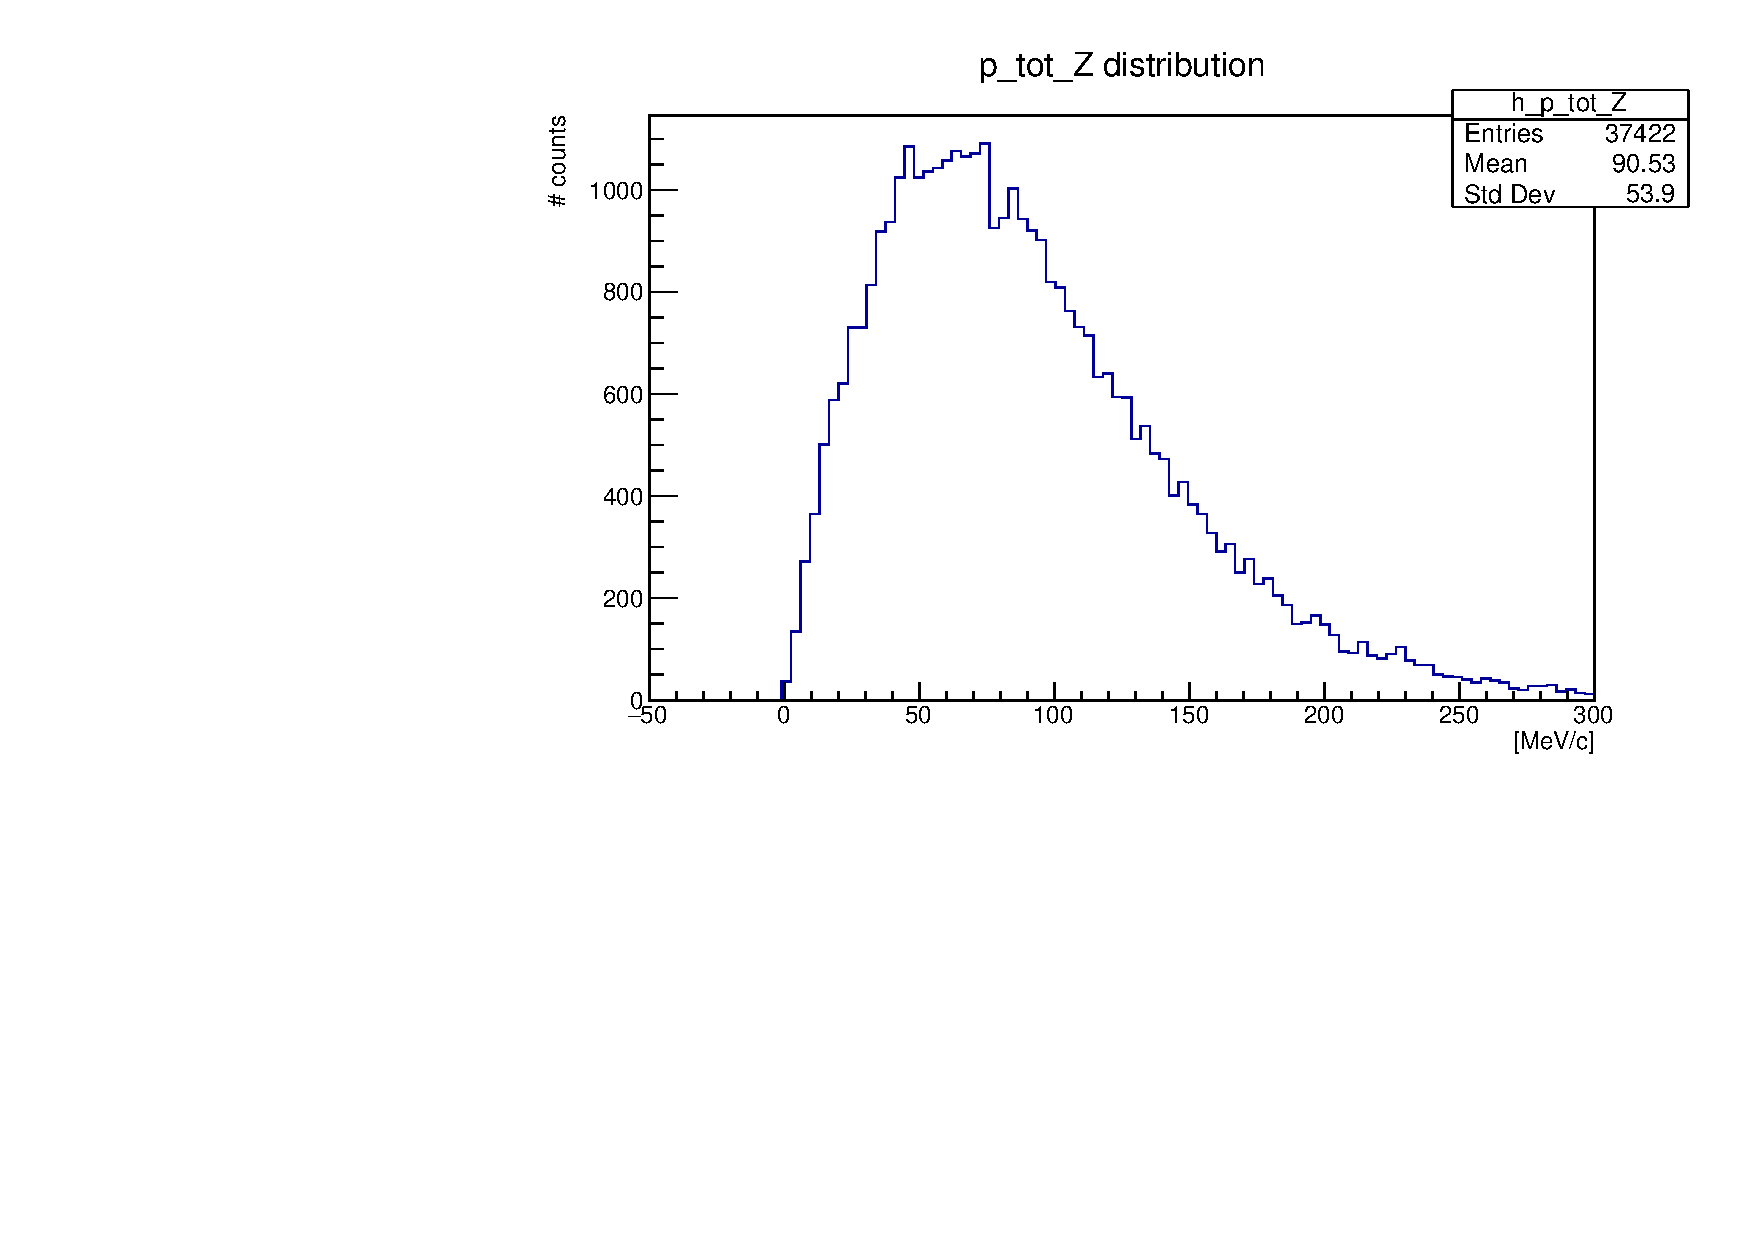
\includegraphics[scale=0.7]{p_tot_Z.pdf} 
\caption{Impulso totale della $Z$.} 
\end{figure}

\begin{figure}[h] 
\centering 
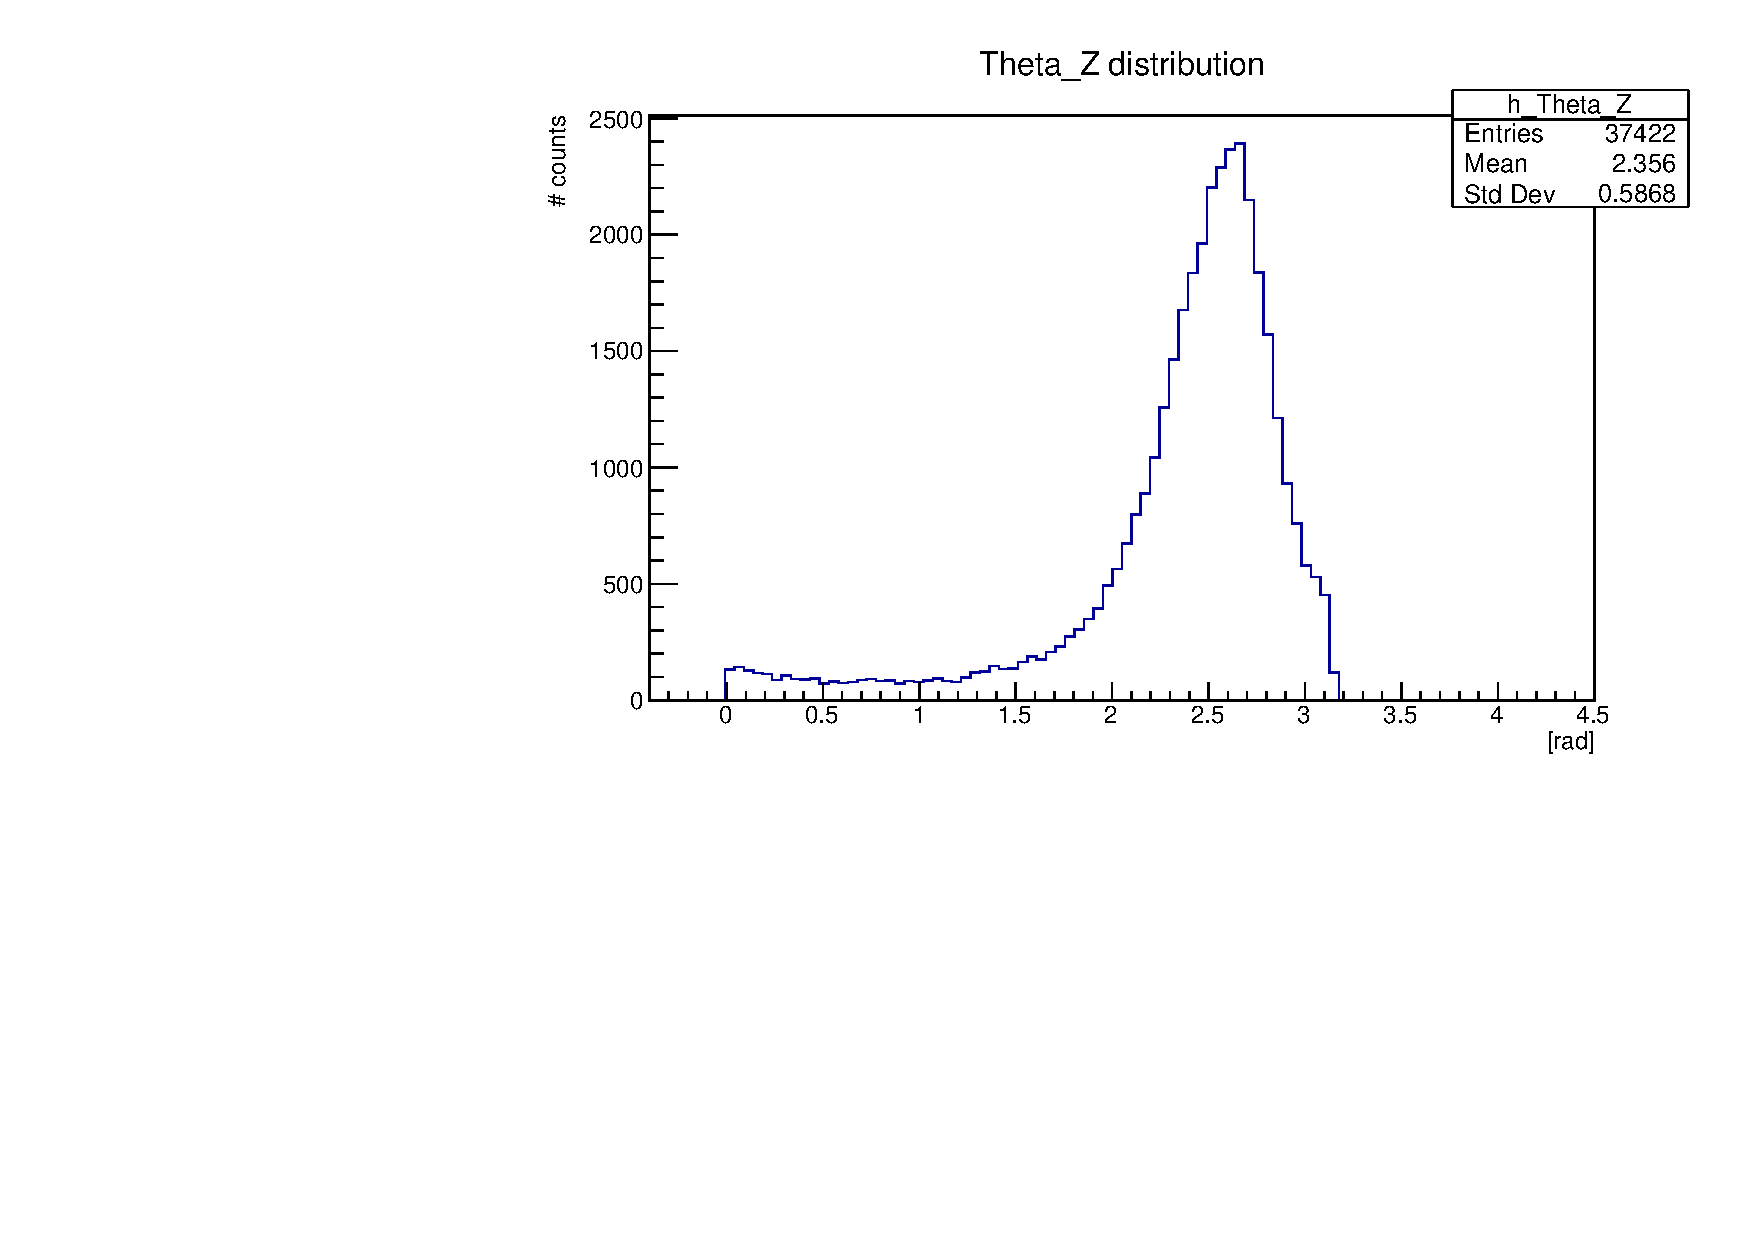
\includegraphics[scale=0.7]{Theta_Z.pdf} 
\caption{Angolo $\theta$ della $Z$.} 
\end{figure}

\begin{figure}[h] 
\centering 
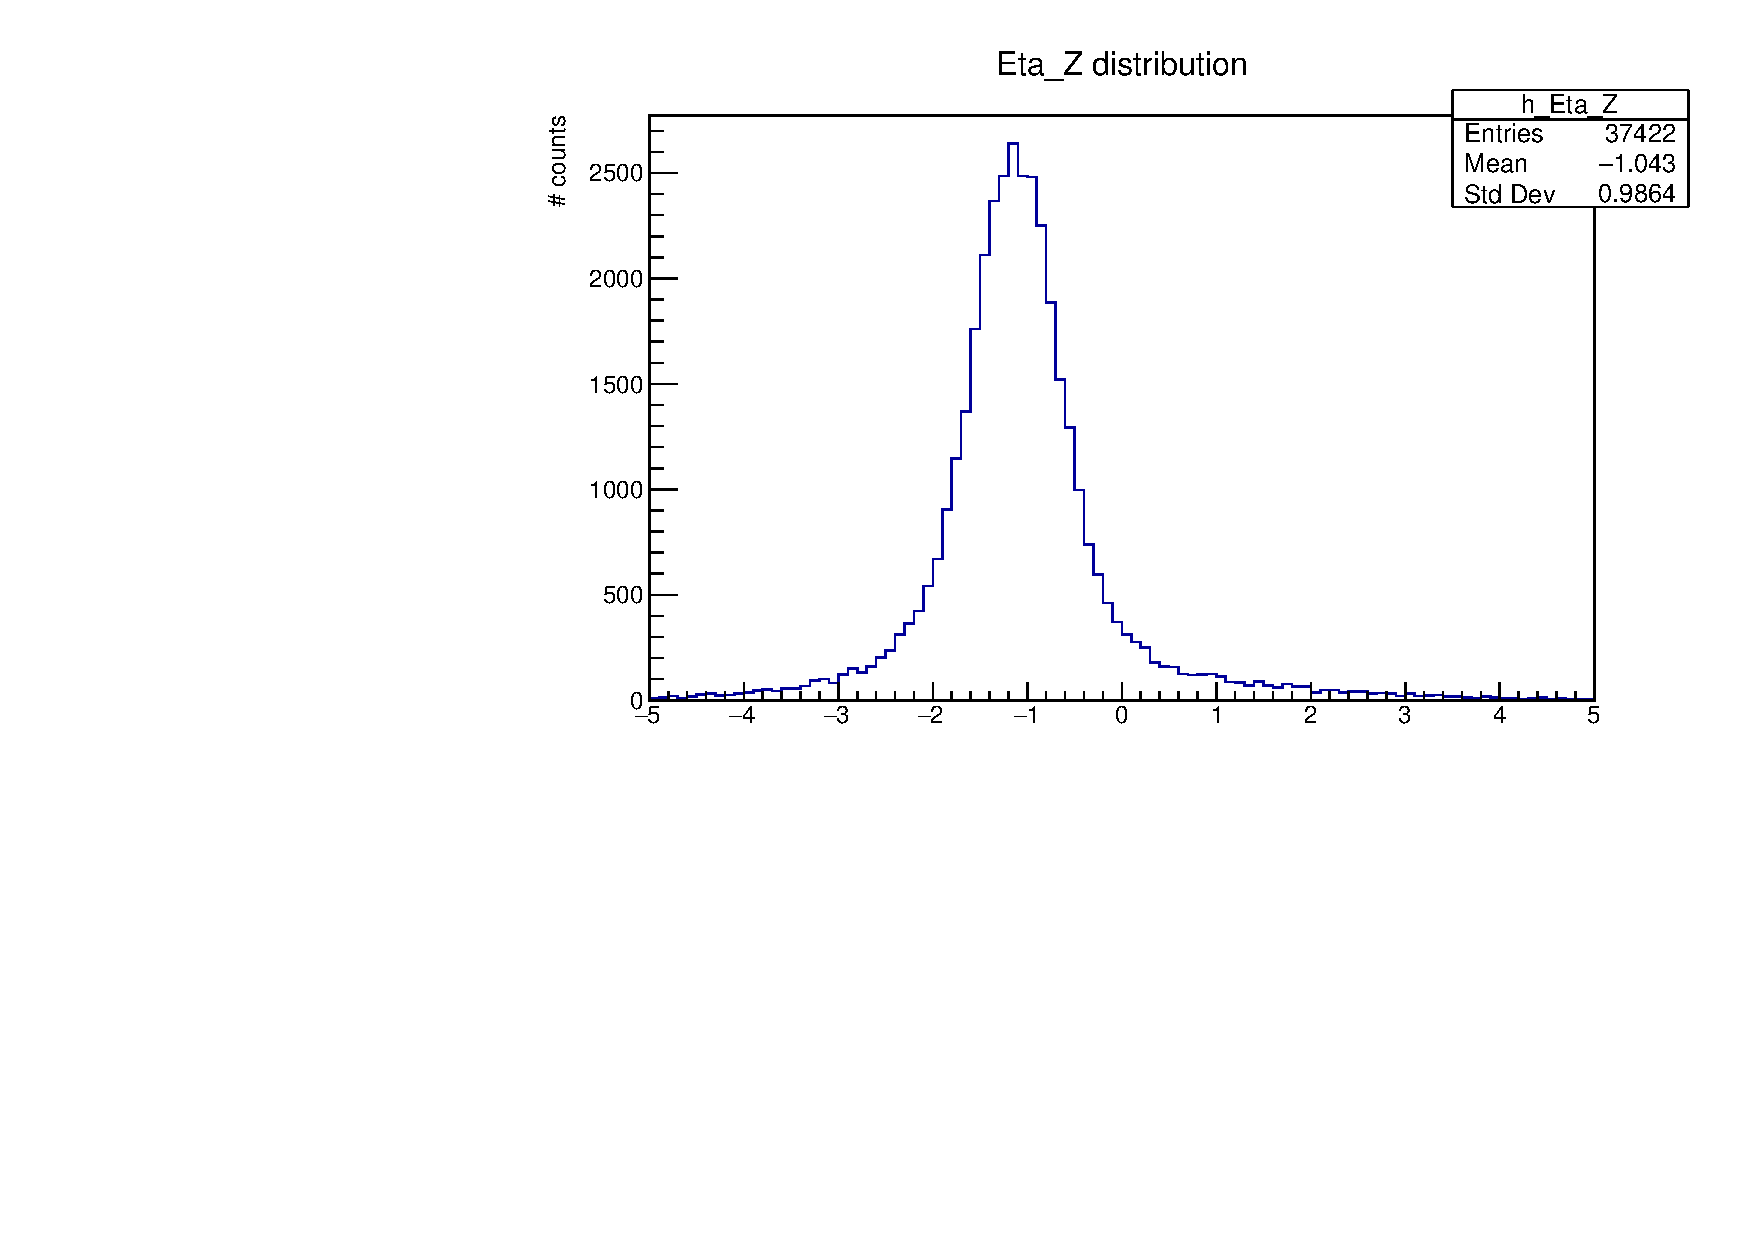
\includegraphics[scale=0.7]{Eta_Z.pdf} 
\caption{Pseudo-rapidit\'a della $Z$.} 
\end{figure}
\clearpage
%%%%%%%%%%%%%%%%%%%%%%%%%%%%%%%
%\subsection{Istogrammi a confronto}

\begin{figure}
\begin{minipage}[t]{8.5cm}
\centering
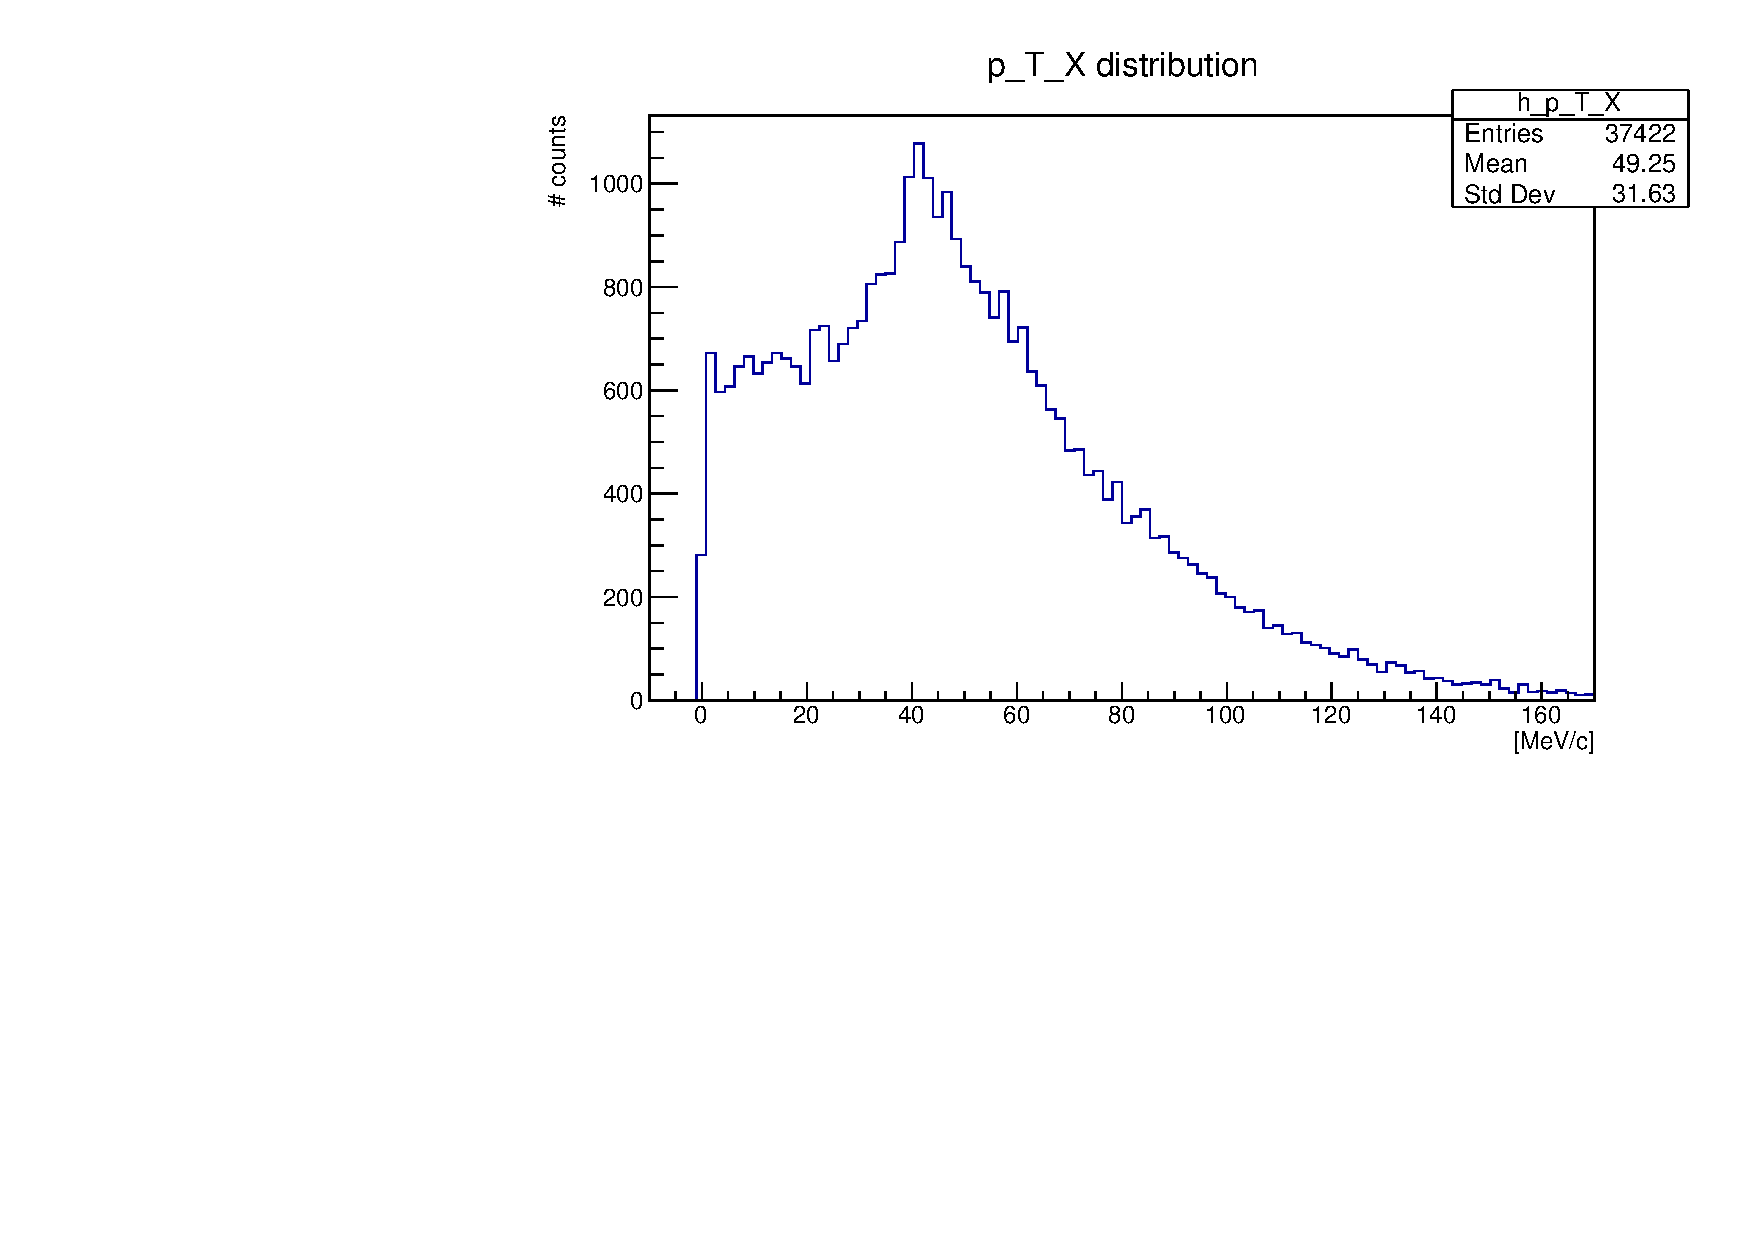
\includegraphics[width=9cm]{p_T_X.pdf}
%\caption{Prima figura}
\end{minipage}
\ \hspace{1mm} \hspace{1mm} \
\begin{minipage}[b]{8.5cm}
\centering
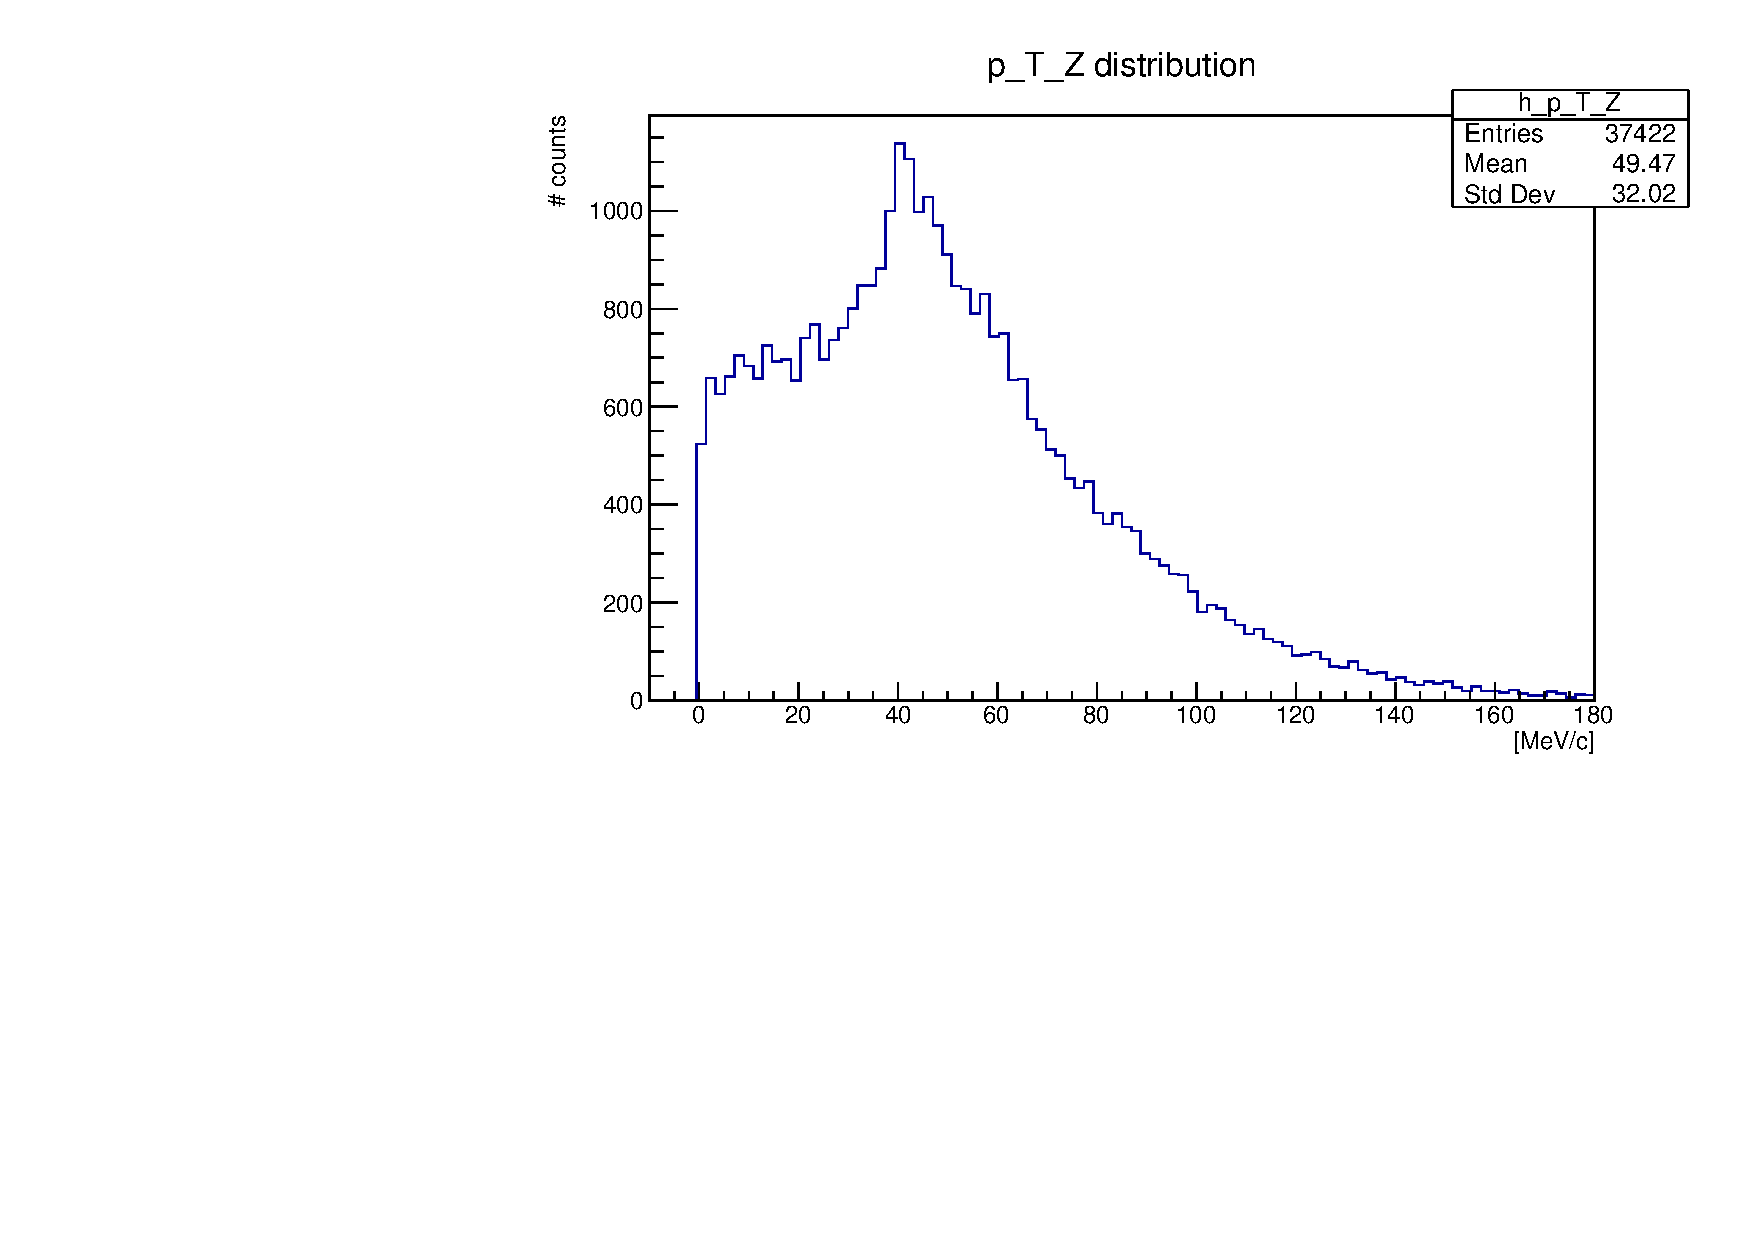
\includegraphics[width=9cm]{p_T_Z.pdf}
%\caption{Seconda figura}
\end{minipage}
\end{figure}

\begin{figure}
\begin{minipage}[b]{8.5cm}
\centering
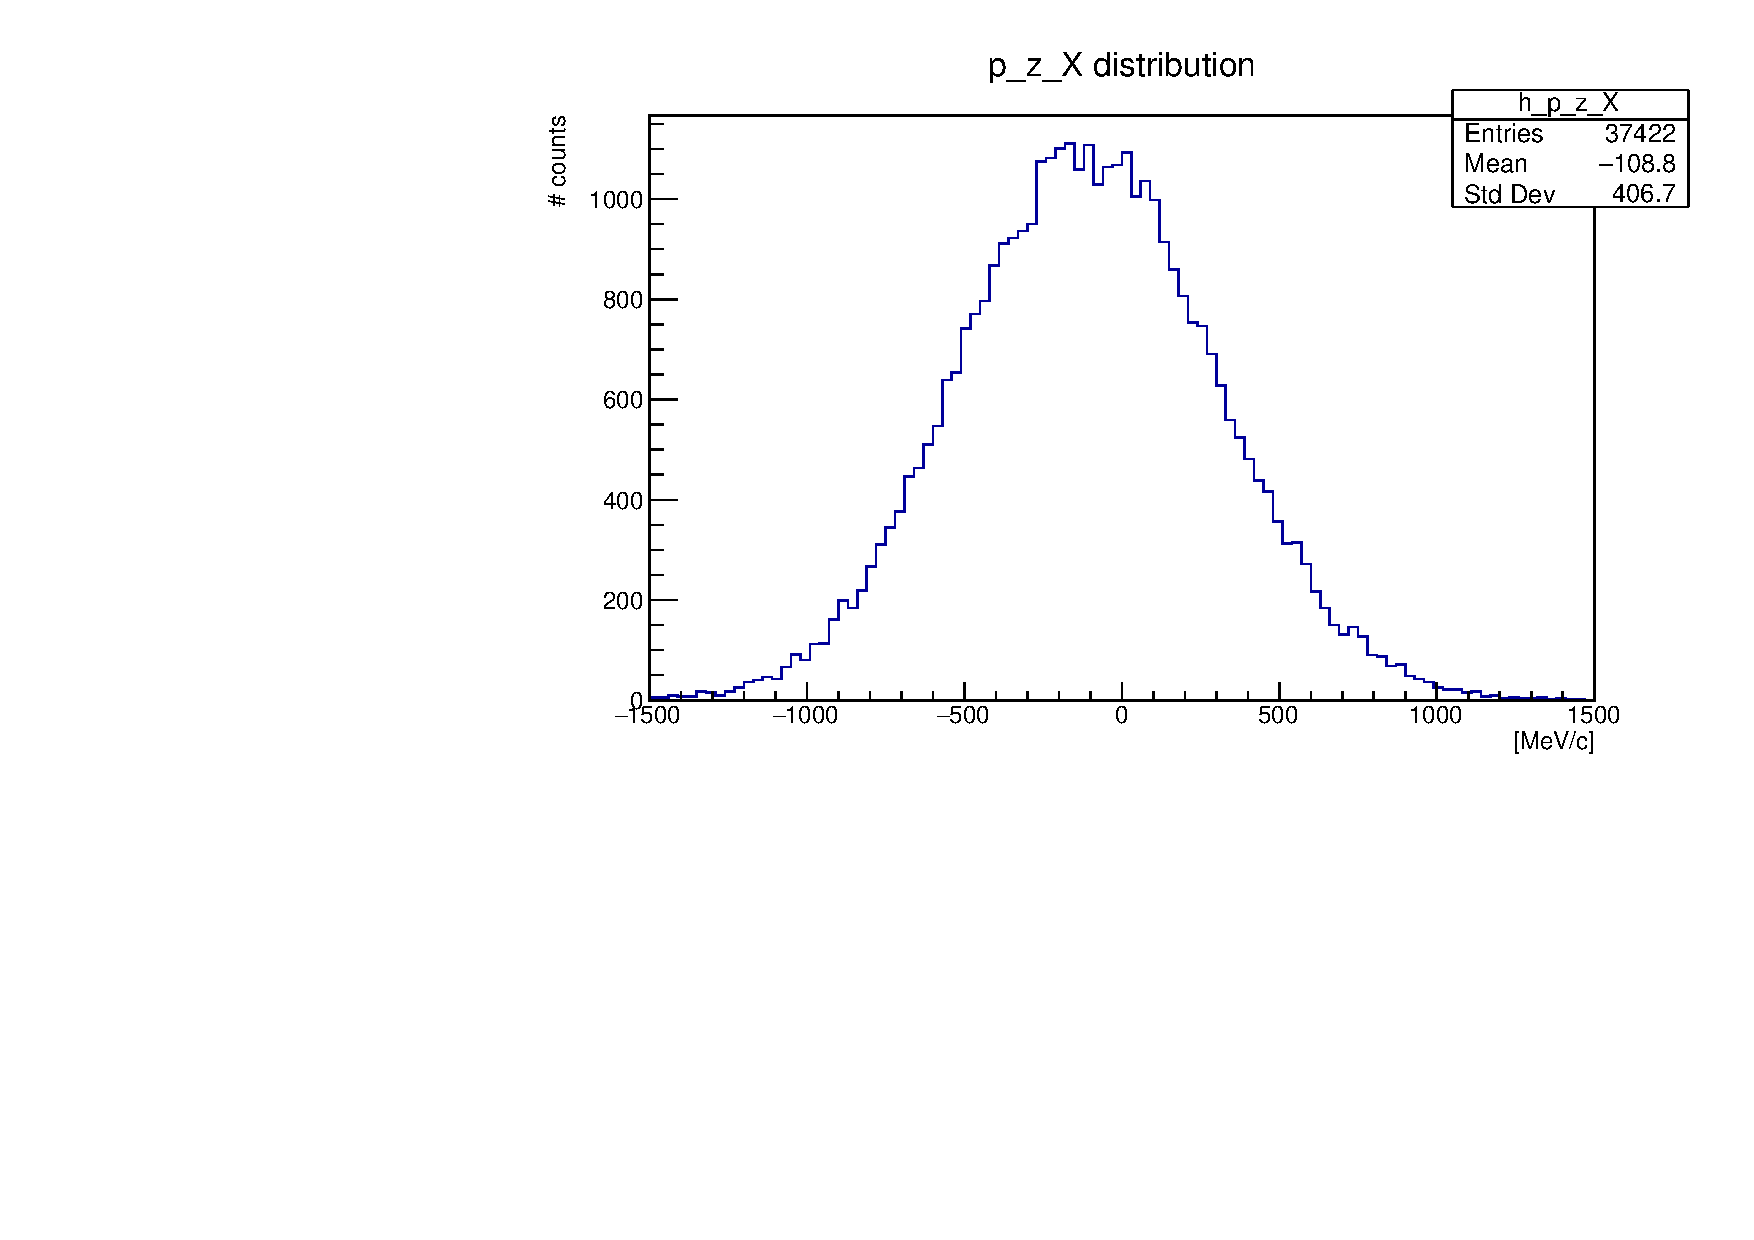
\includegraphics[width=9cm]{p_z_X.pdf}
%\caption{Prima figura}
\end{minipage}
\ \hspace{1mm} \hspace{1mm} \
\begin{minipage}[b]{8.5cm}
\centering
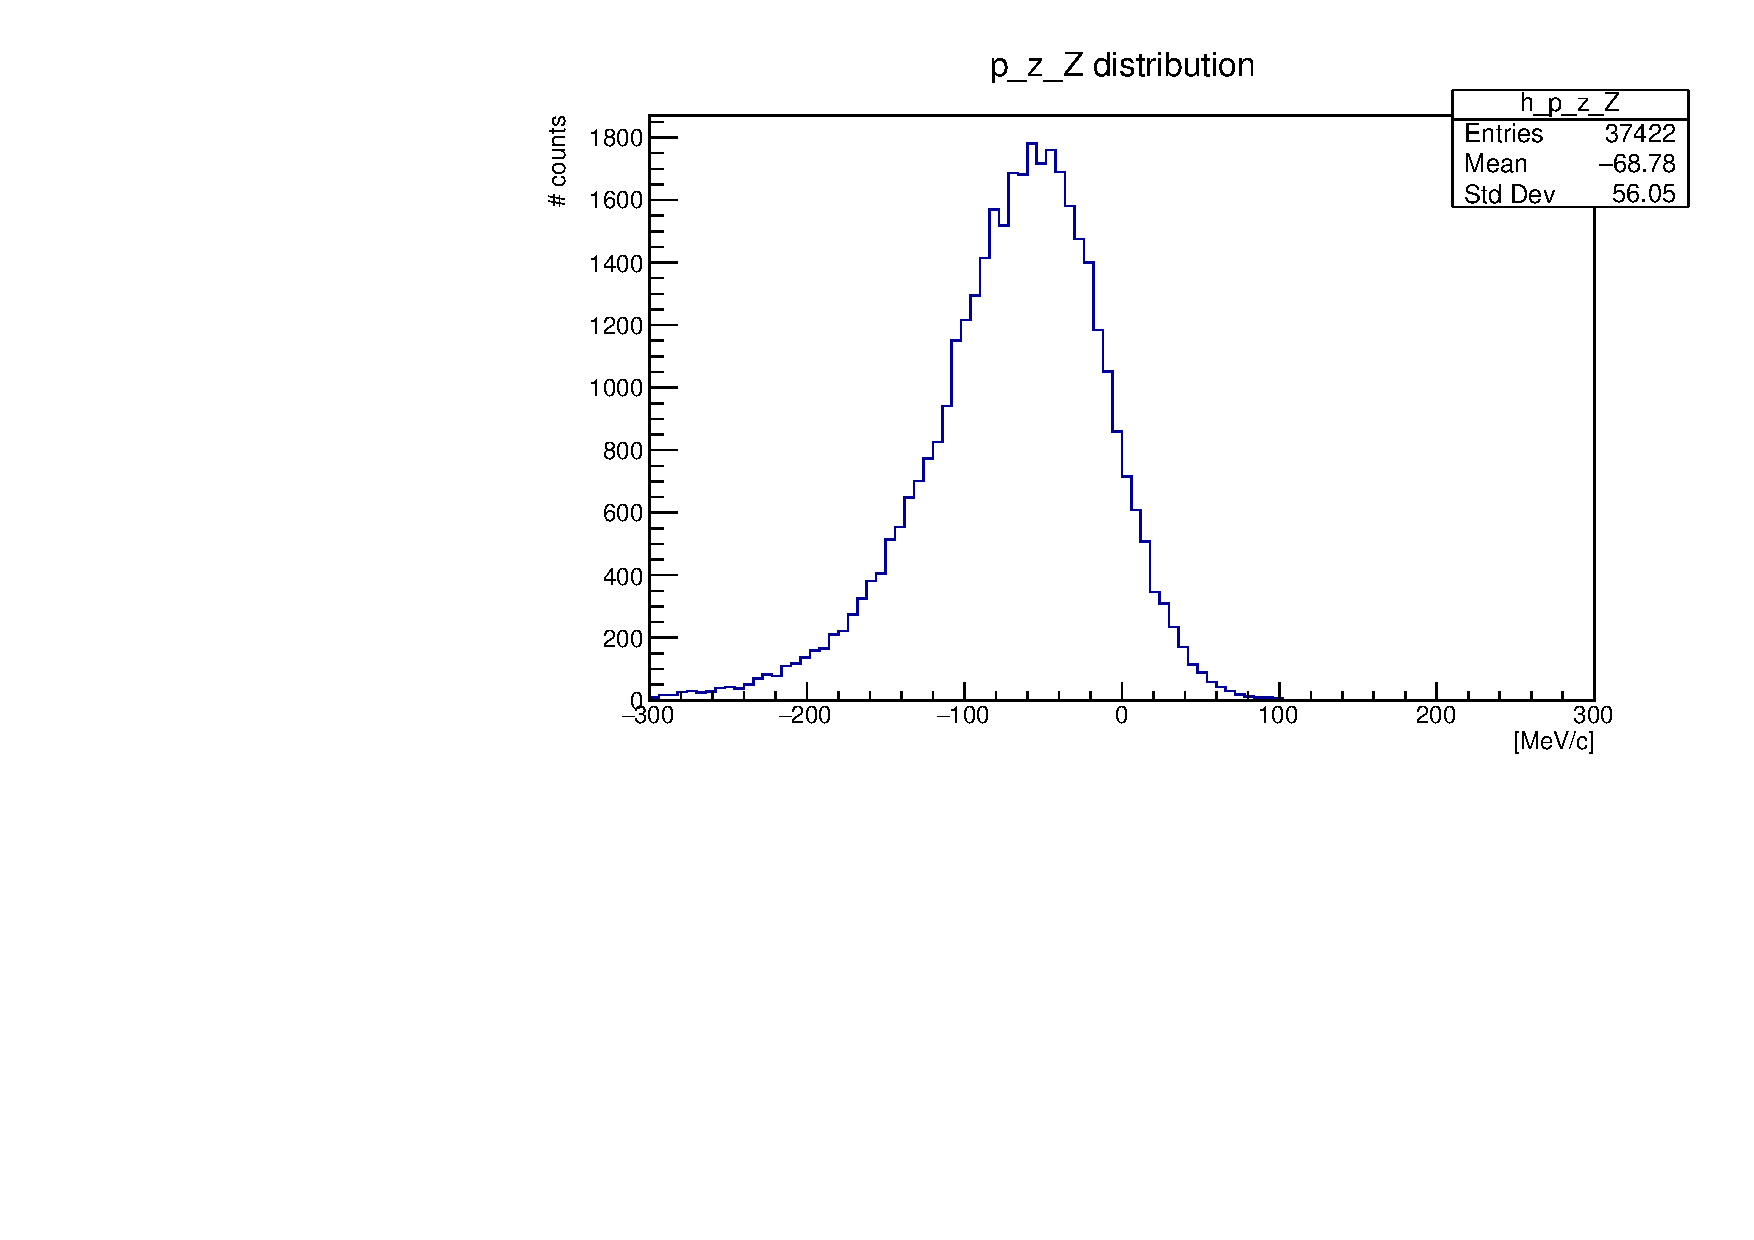
\includegraphics[width=9cm]{p_z_Z.pdf}
%\caption{Seconda figura}
\end{minipage}
\end{figure}

\begin{figure}
\begin{minipage}[b]{8.5cm}
\centering
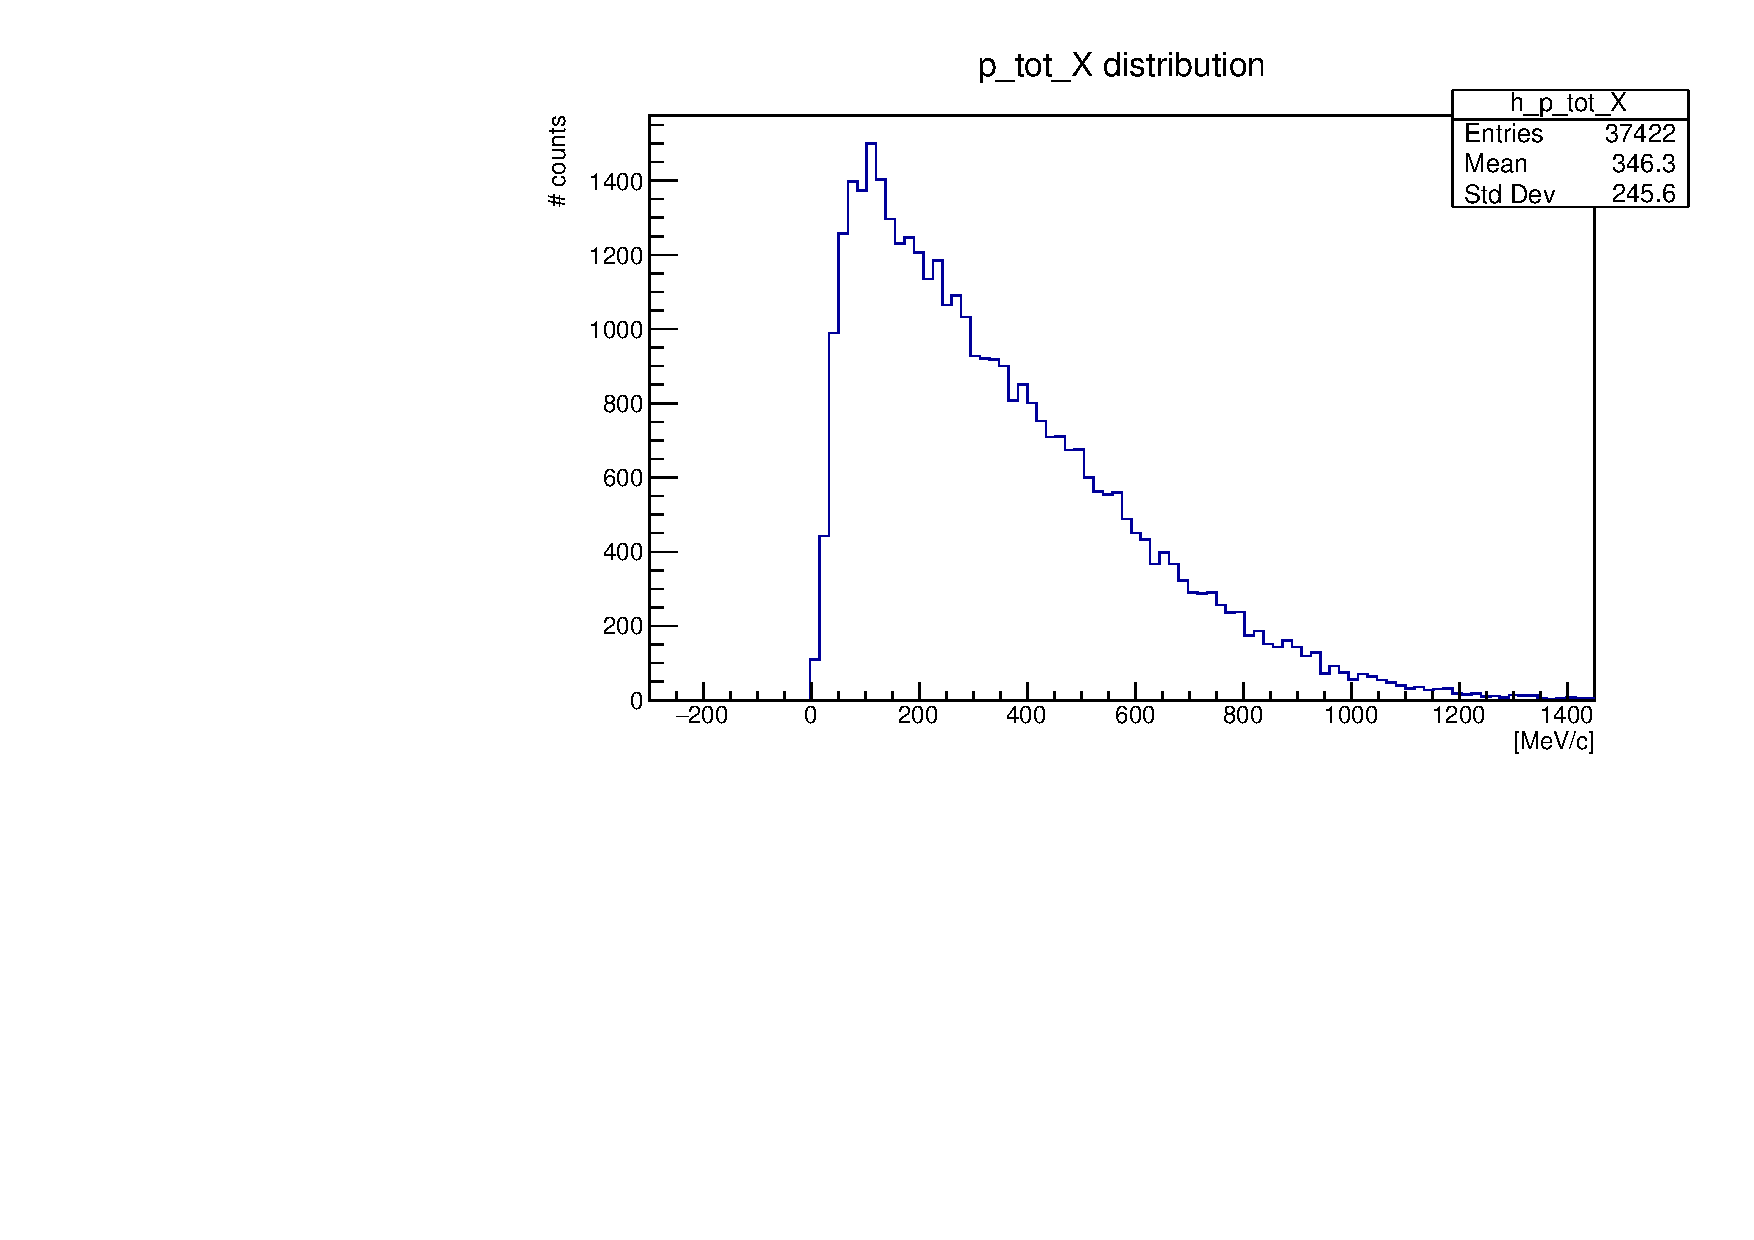
\includegraphics[width=9cm]{p_tot_X.pdf}
%\caption{Prima figura}
\end{minipage}
\ \hspace{1mm} \hspace{1mm} \
\begin{minipage}[b]{8.5cm}
\centering
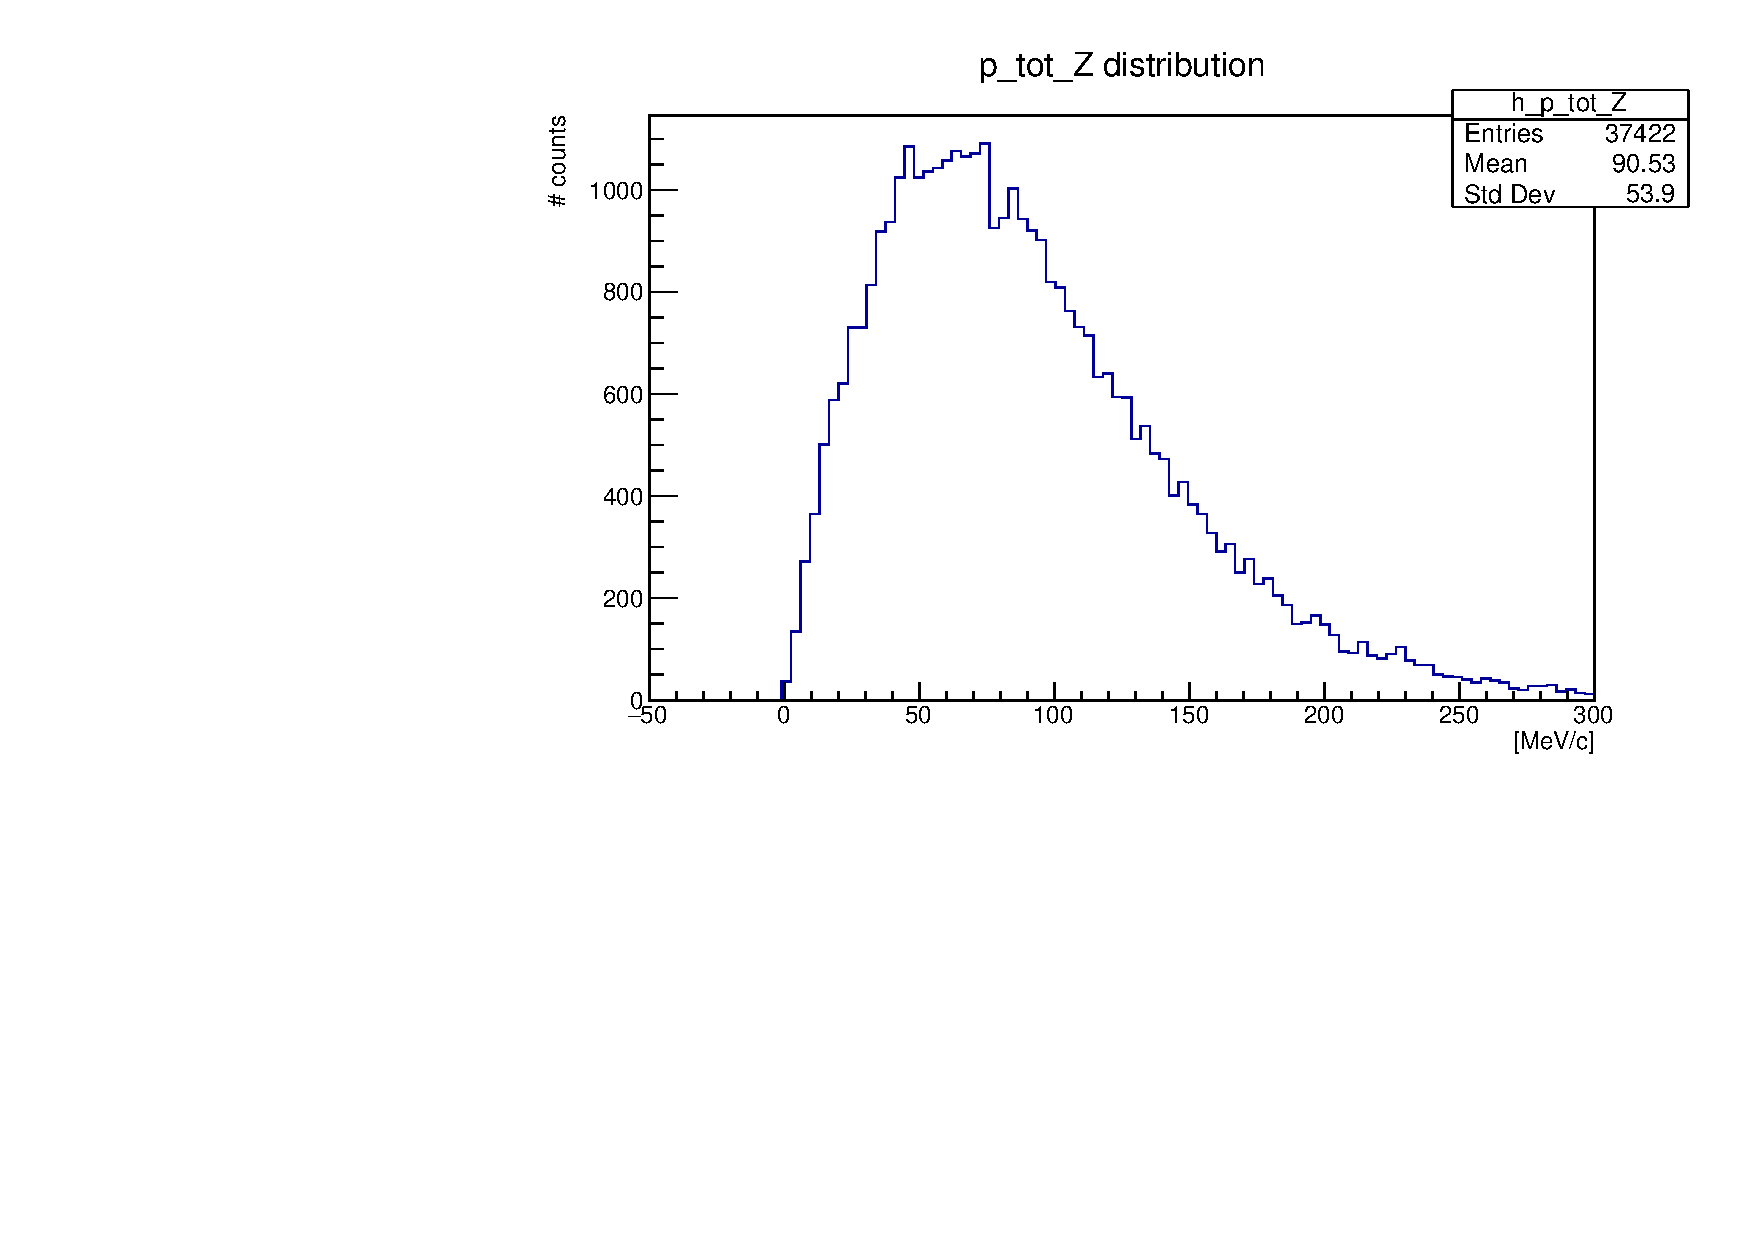
\includegraphics[width=9cm]{p_tot_Z.pdf}
%\caption{Seconda figura}
\end{minipage}
\end{figure}

\begin{figure}
\begin{minipage}[b]{8.5cm}
\centering
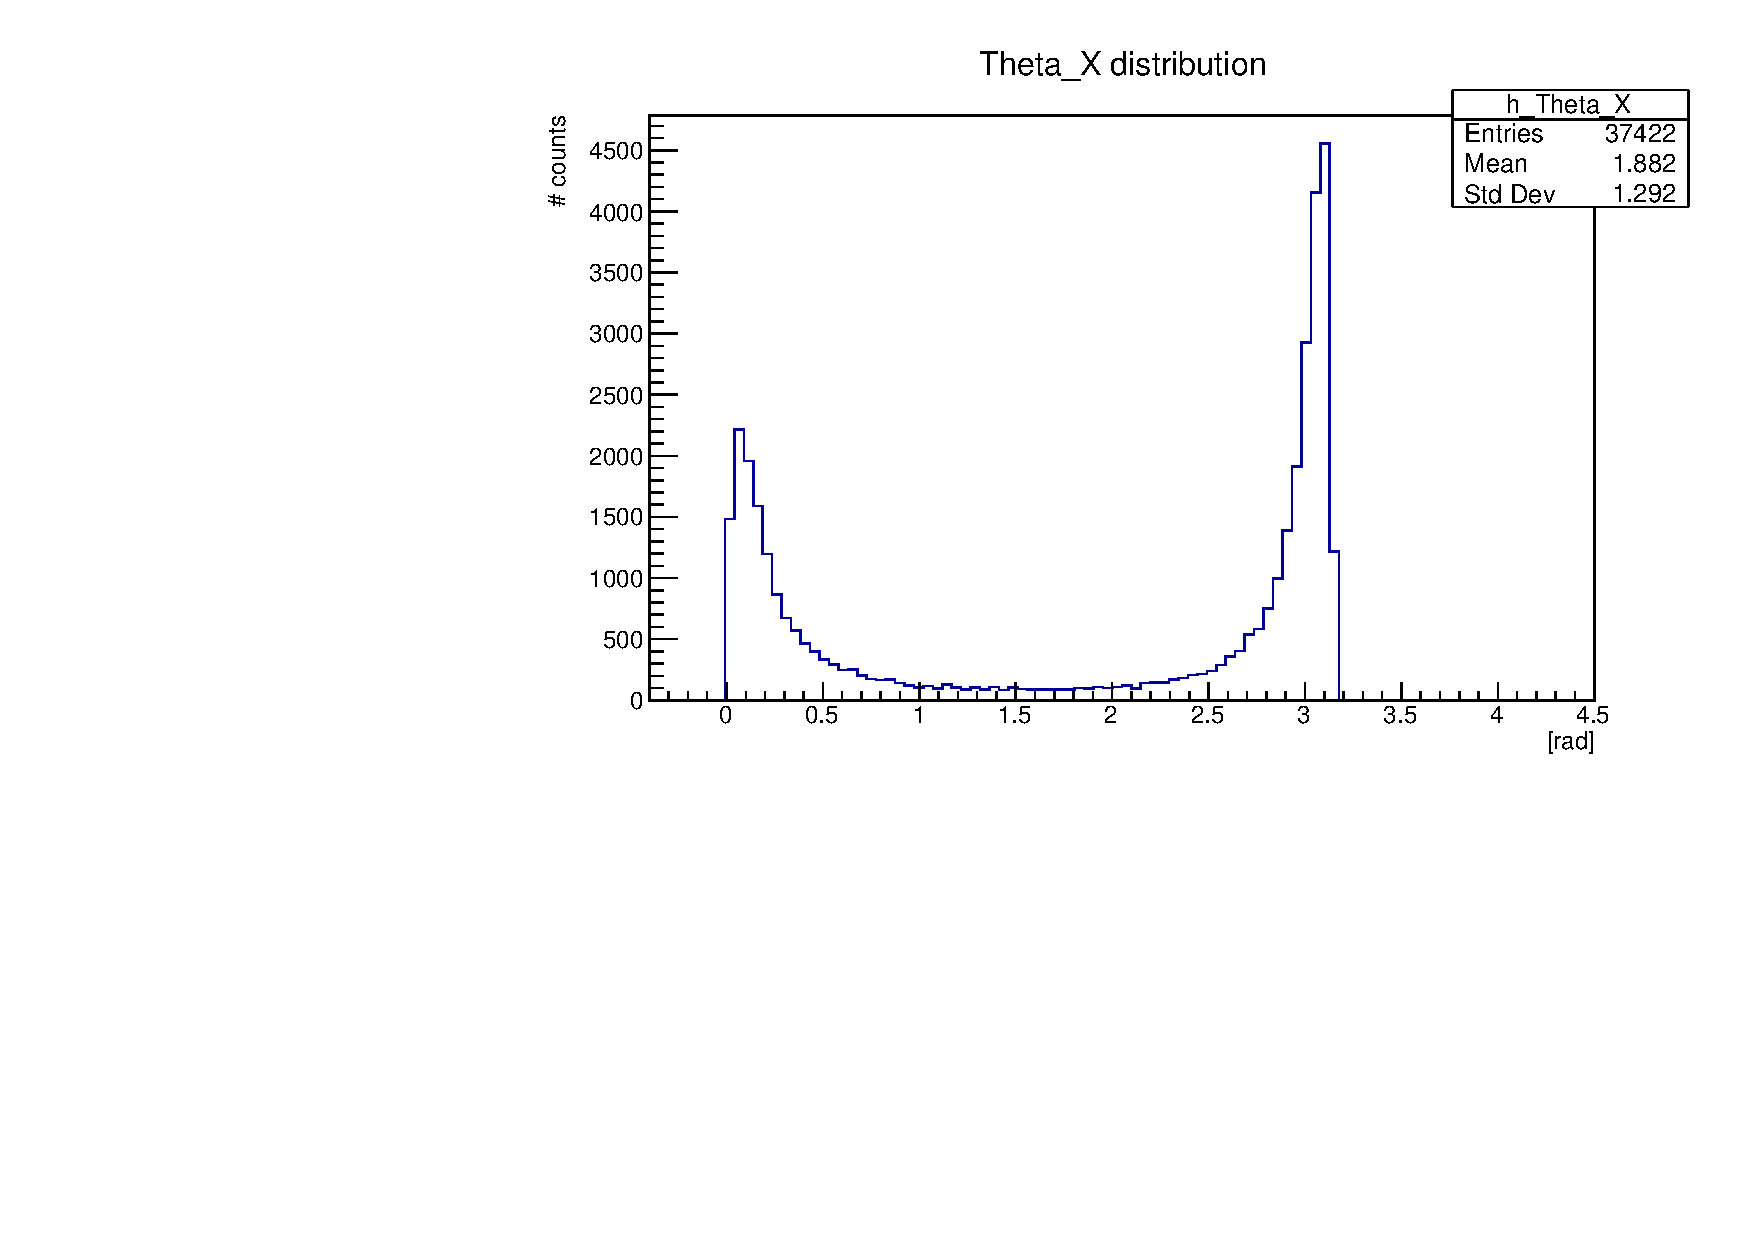
\includegraphics[width=9cm]{Theta_X.pdf}
%\caption{Prima figura}
\end{minipage}
\ \hspace{1mm} \hspace{1mm} \
\begin{minipage}[b]{8.5cm}
\centering
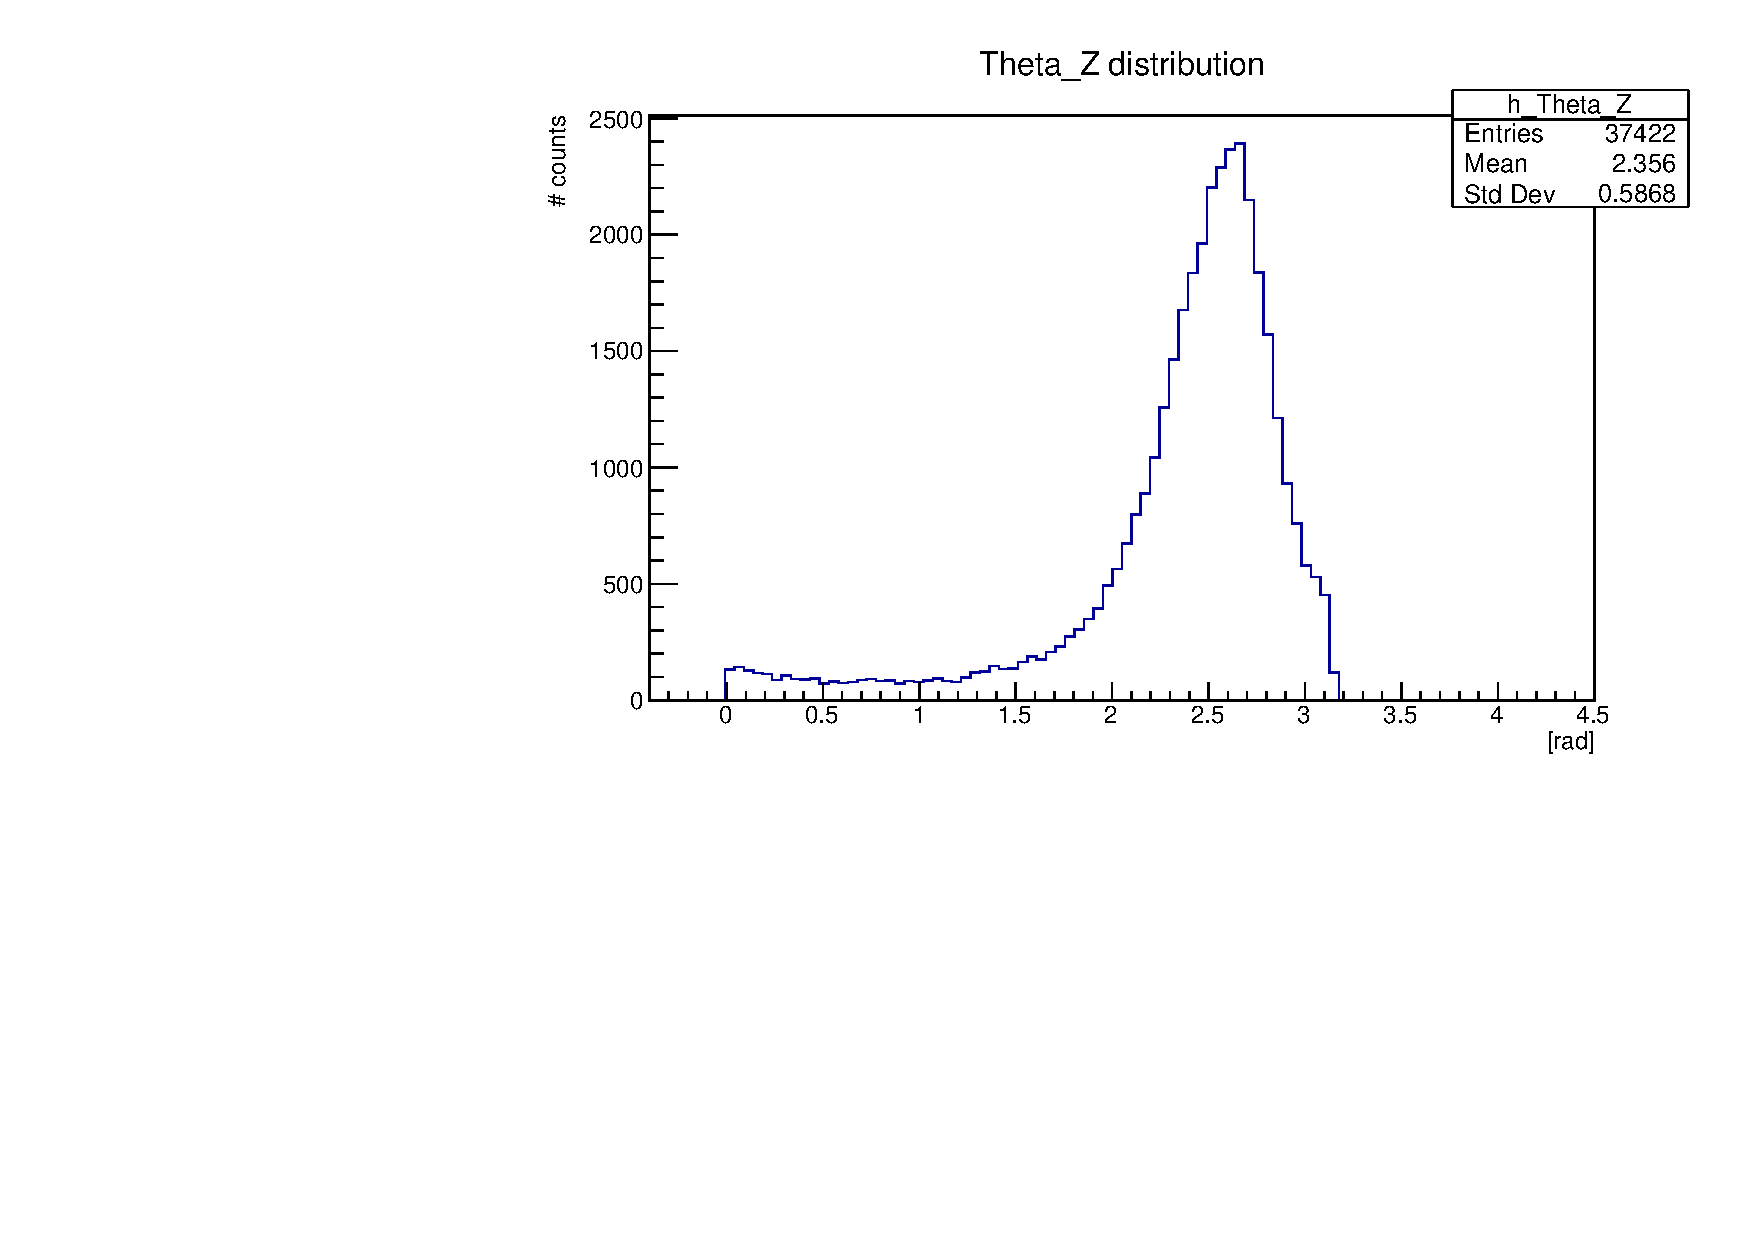
\includegraphics[width=9cm]{Theta_Z.pdf}
%\caption{Seconda figura}
\end{minipage}
\end{figure}

\begin{figure}
\begin{minipage}[b]{8.5cm}
\centering
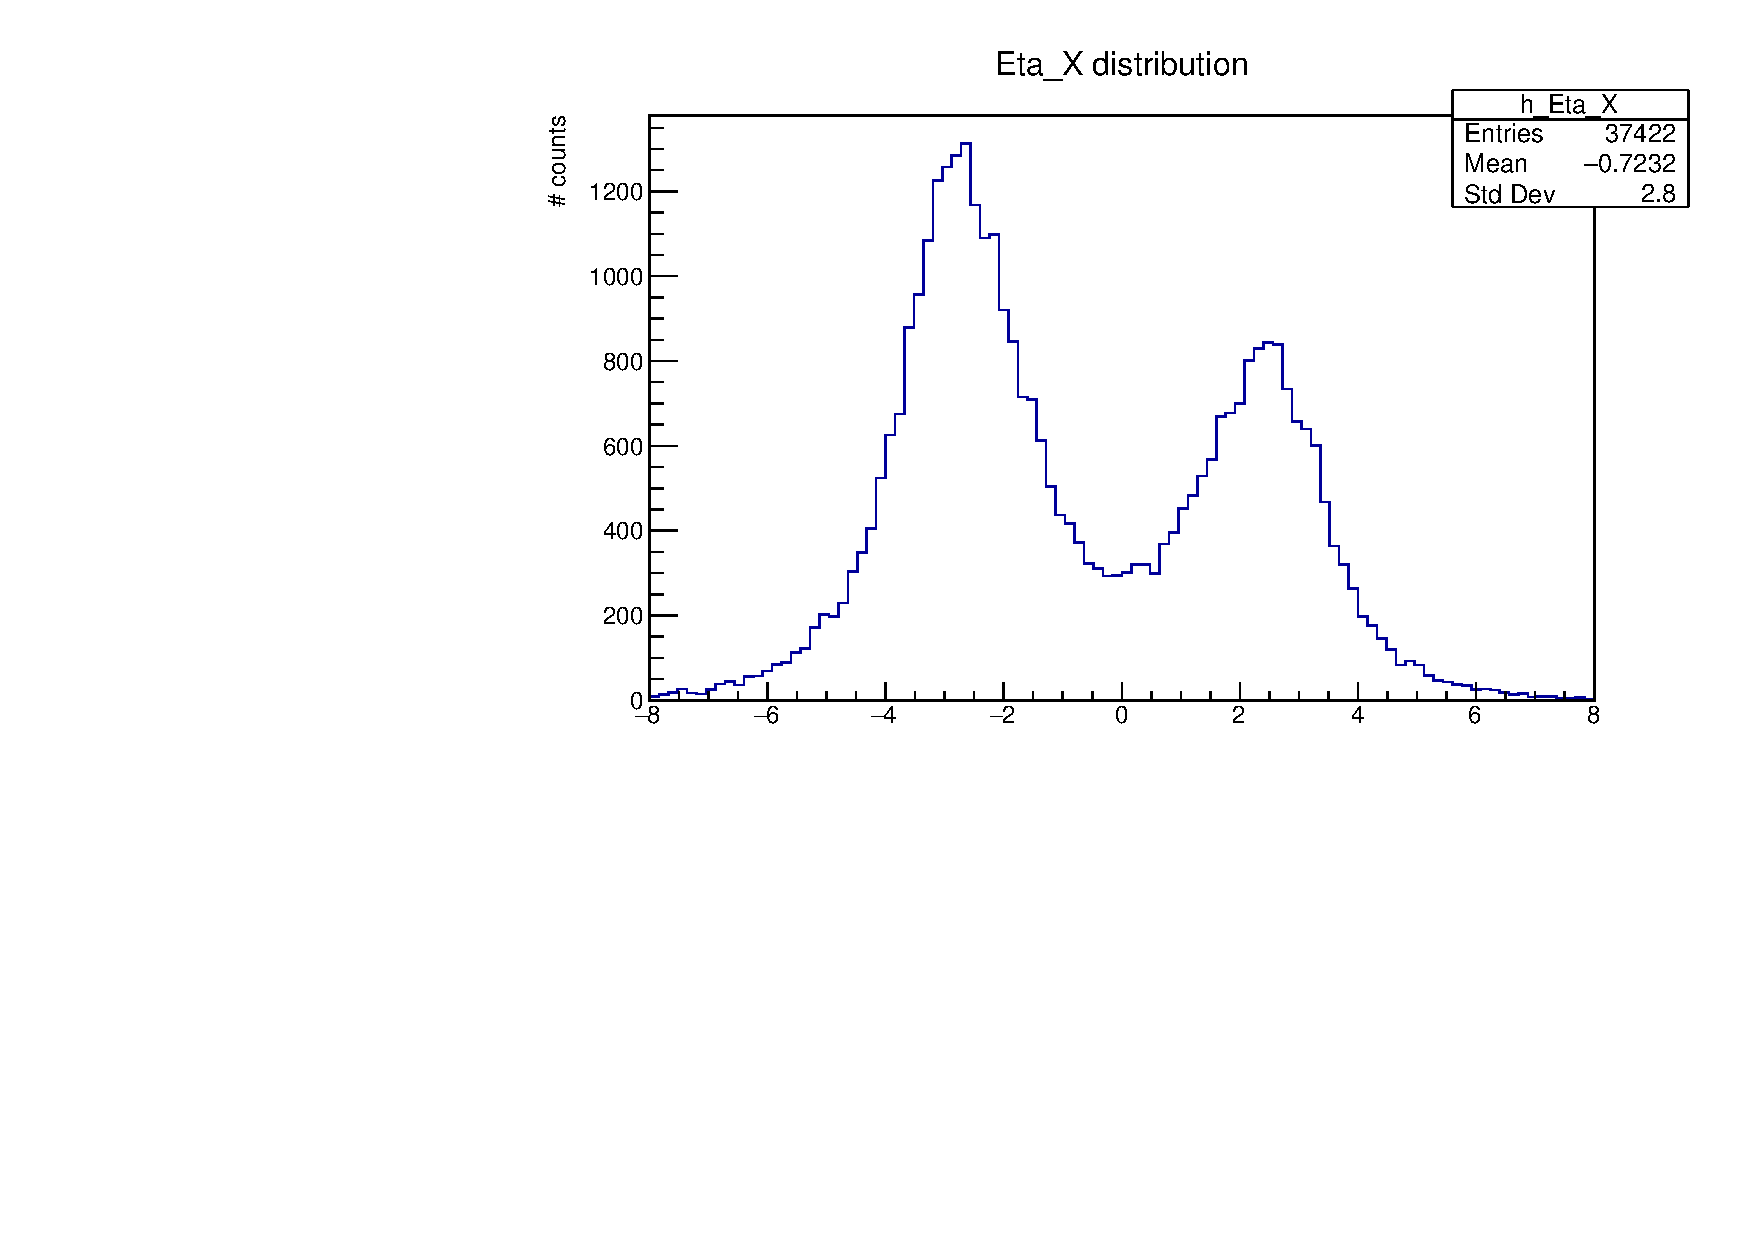
\includegraphics[width=9cm]{Eta_X.pdf}
%\caption{Prima figura}
\end{minipage}
\ \hspace{1mm} \hspace{1mm} \
\begin{minipage}[b]{8.5cm}
\centering
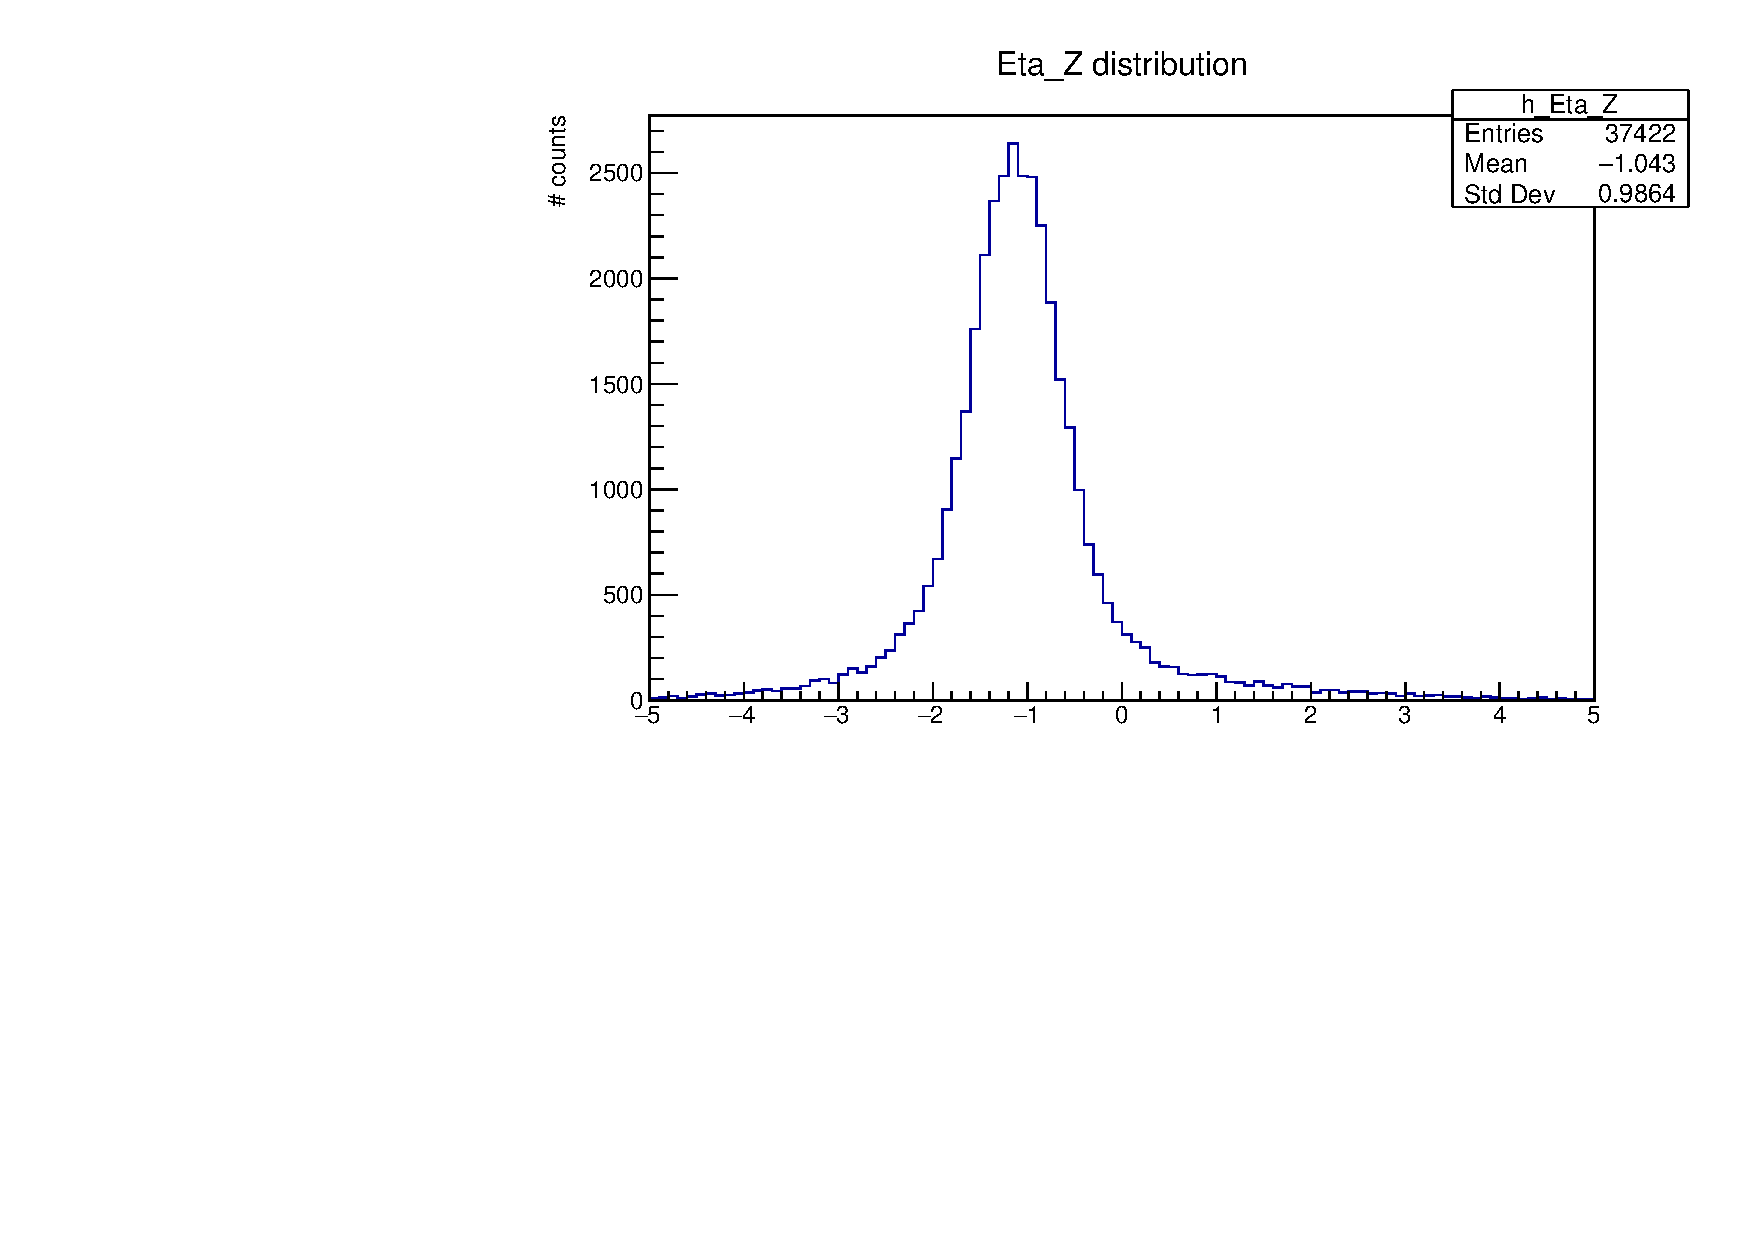
\includegraphics[width=9cm]{Eta_Z.pdf}
%\caption{Seconda figura}
\end{minipage}
\end{figure}

\clearpage
\newpage

\section{Misura dei protoni con i Roman Pot}


Per generare protoni a differenti valori di ($|t|$, $\xi$) si utilizza un simulatore, una \newline"particle-gun" basata su \texttt{LorenzoGenerator.cc}.
Le particelle assumono determinati valori di $|t|$ e $\xi$ si propagano  verso i rivelatori di CT-PPS posizionati a $z$ = 210 m e  \newline
$z$ = 220 m.
Tuttavia  \texttt{LorenzoGenerator.cc} non \'e sufficiente da solo a simulare la distribuzione dei protoni rilevati dai Roman Pot, dal momento che restituisce in output solo i valori di $|t|$ e $\xi$ dei protoni e le grandezze cinematiche delle particelle generate nell'urto $Z$ e $X$. Per tale motivo sono stati sviluppati due ulteriori programmi scritti in linguaggio python, ossia  \texttt{test\_gen\_simu\_cfg.py} e  \texttt{test\_gen\_simu\_smear\_cfg.py}.\newline

\begin{figure}[h!] 
\centering
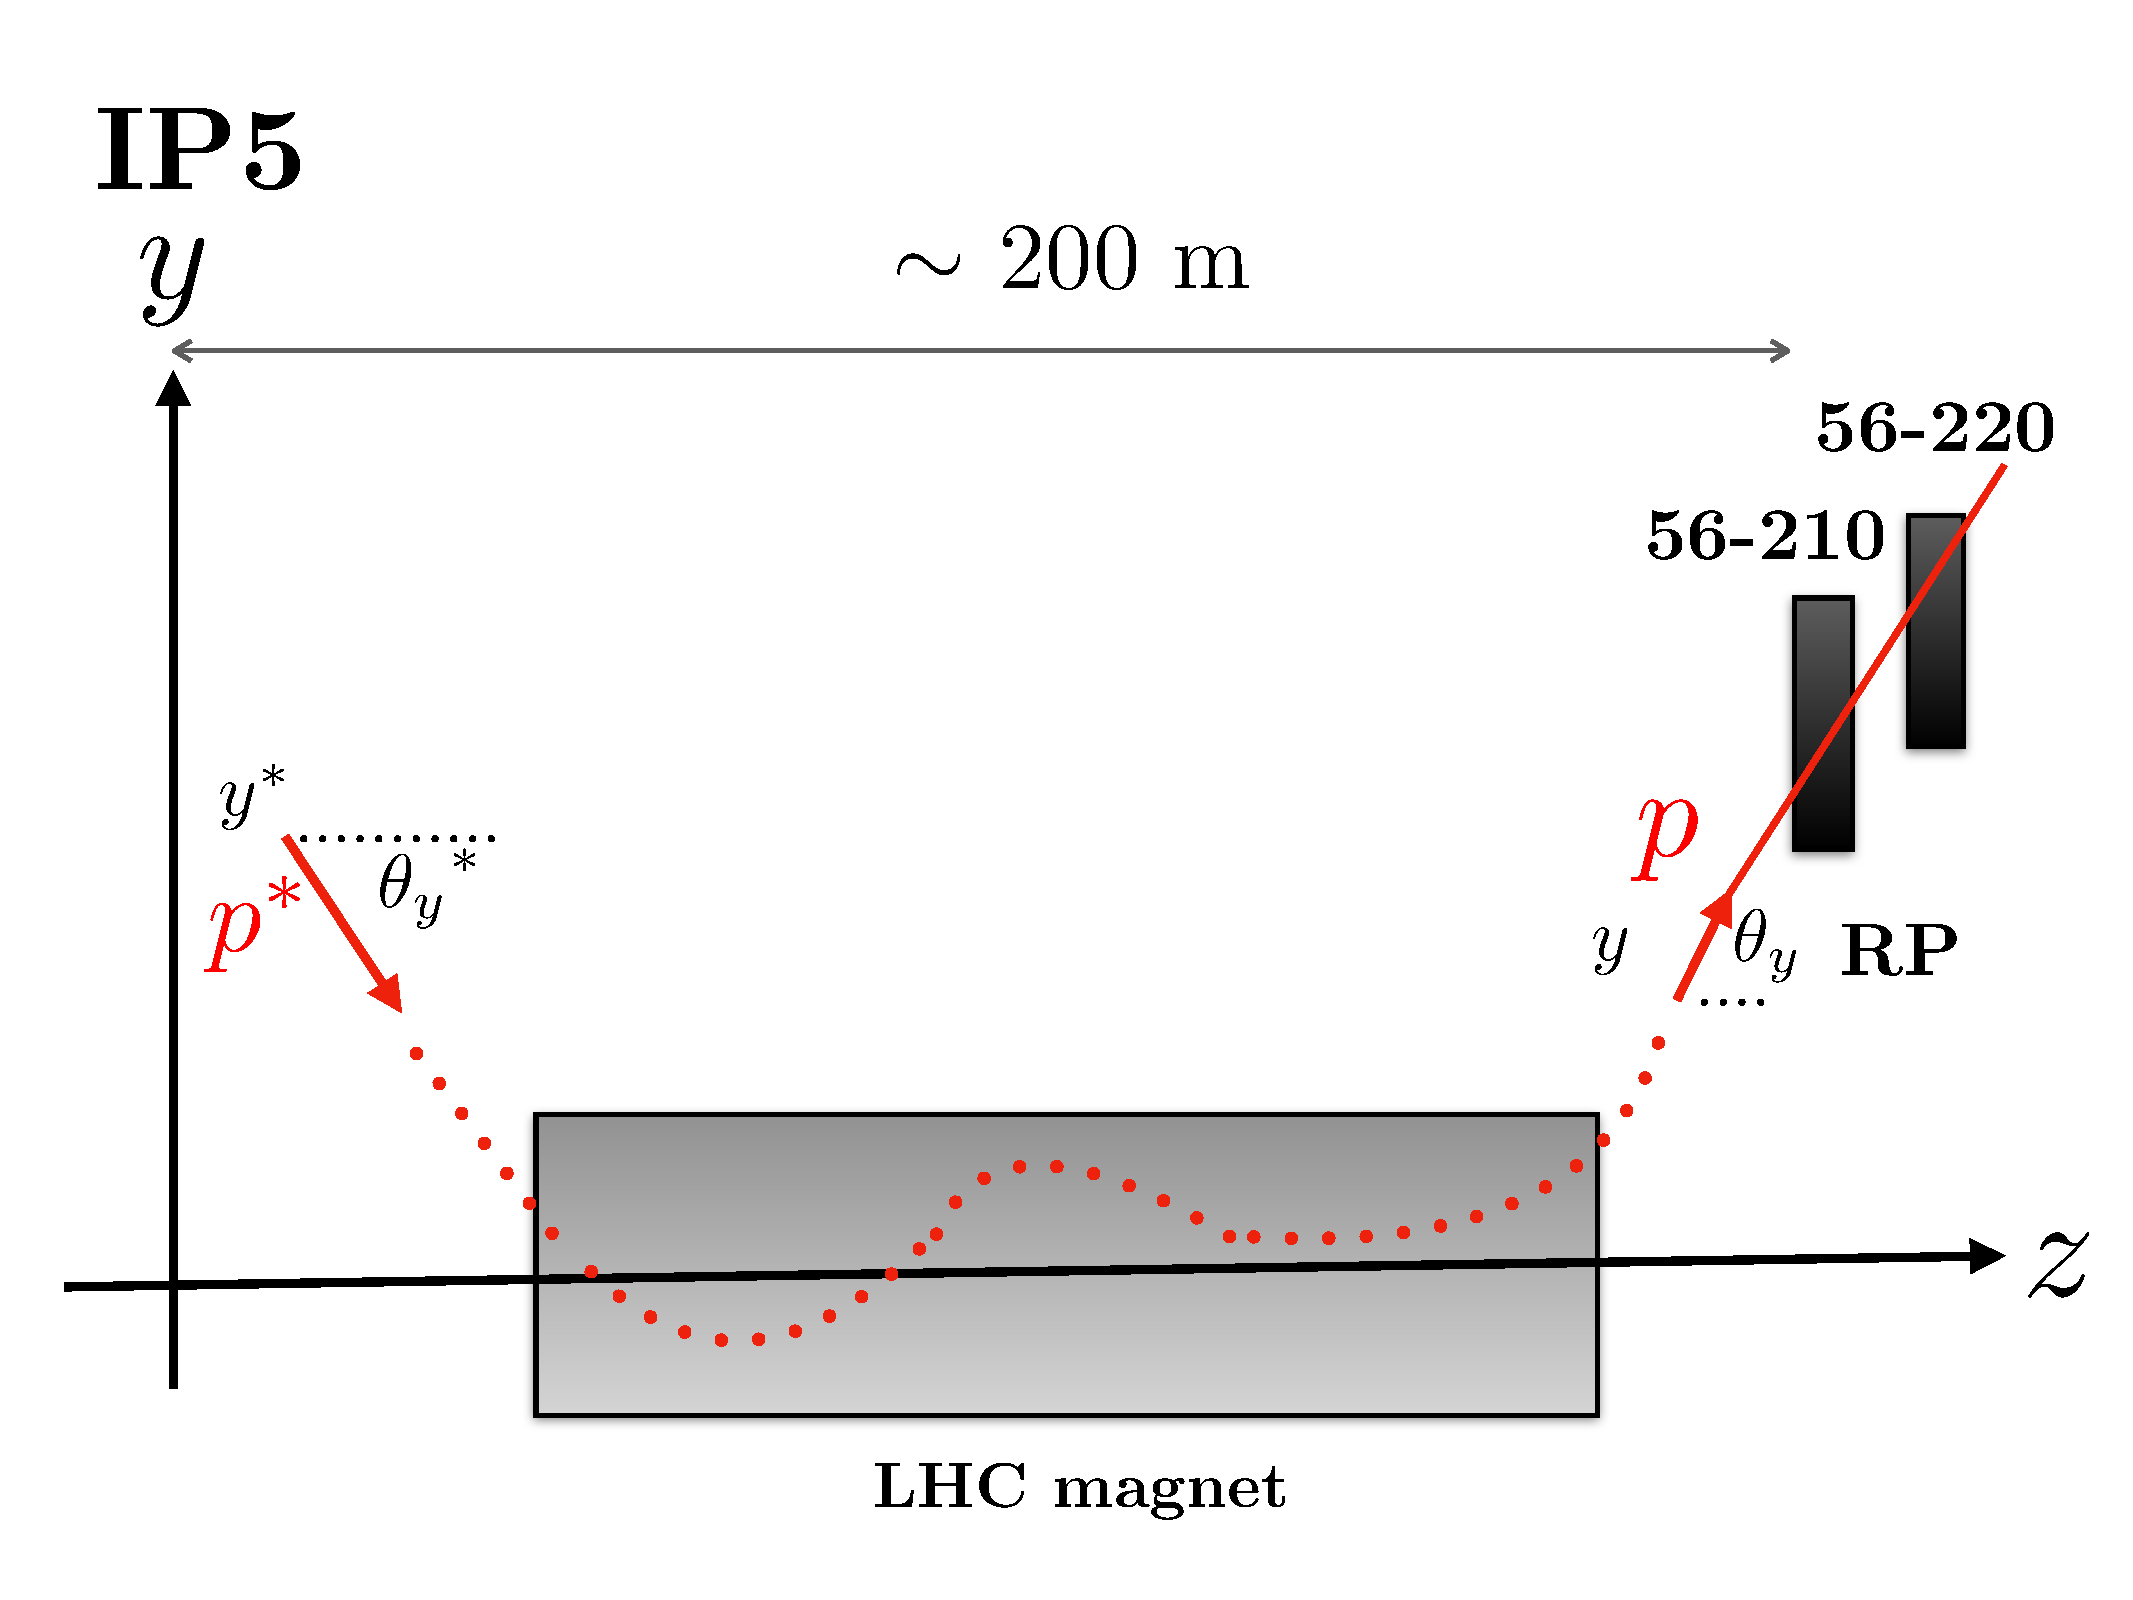
\includegraphics[scale=0.35]{protoni_RP1.pdf} 
\caption{Schema dell'evento fisico simulato. Il protone, proveniente dall'ottante 45 viene rilevato dai RP 56-210 (m) e 56-220 (m).}
\end{figure}
\begin{figure}[h!] 
\centering
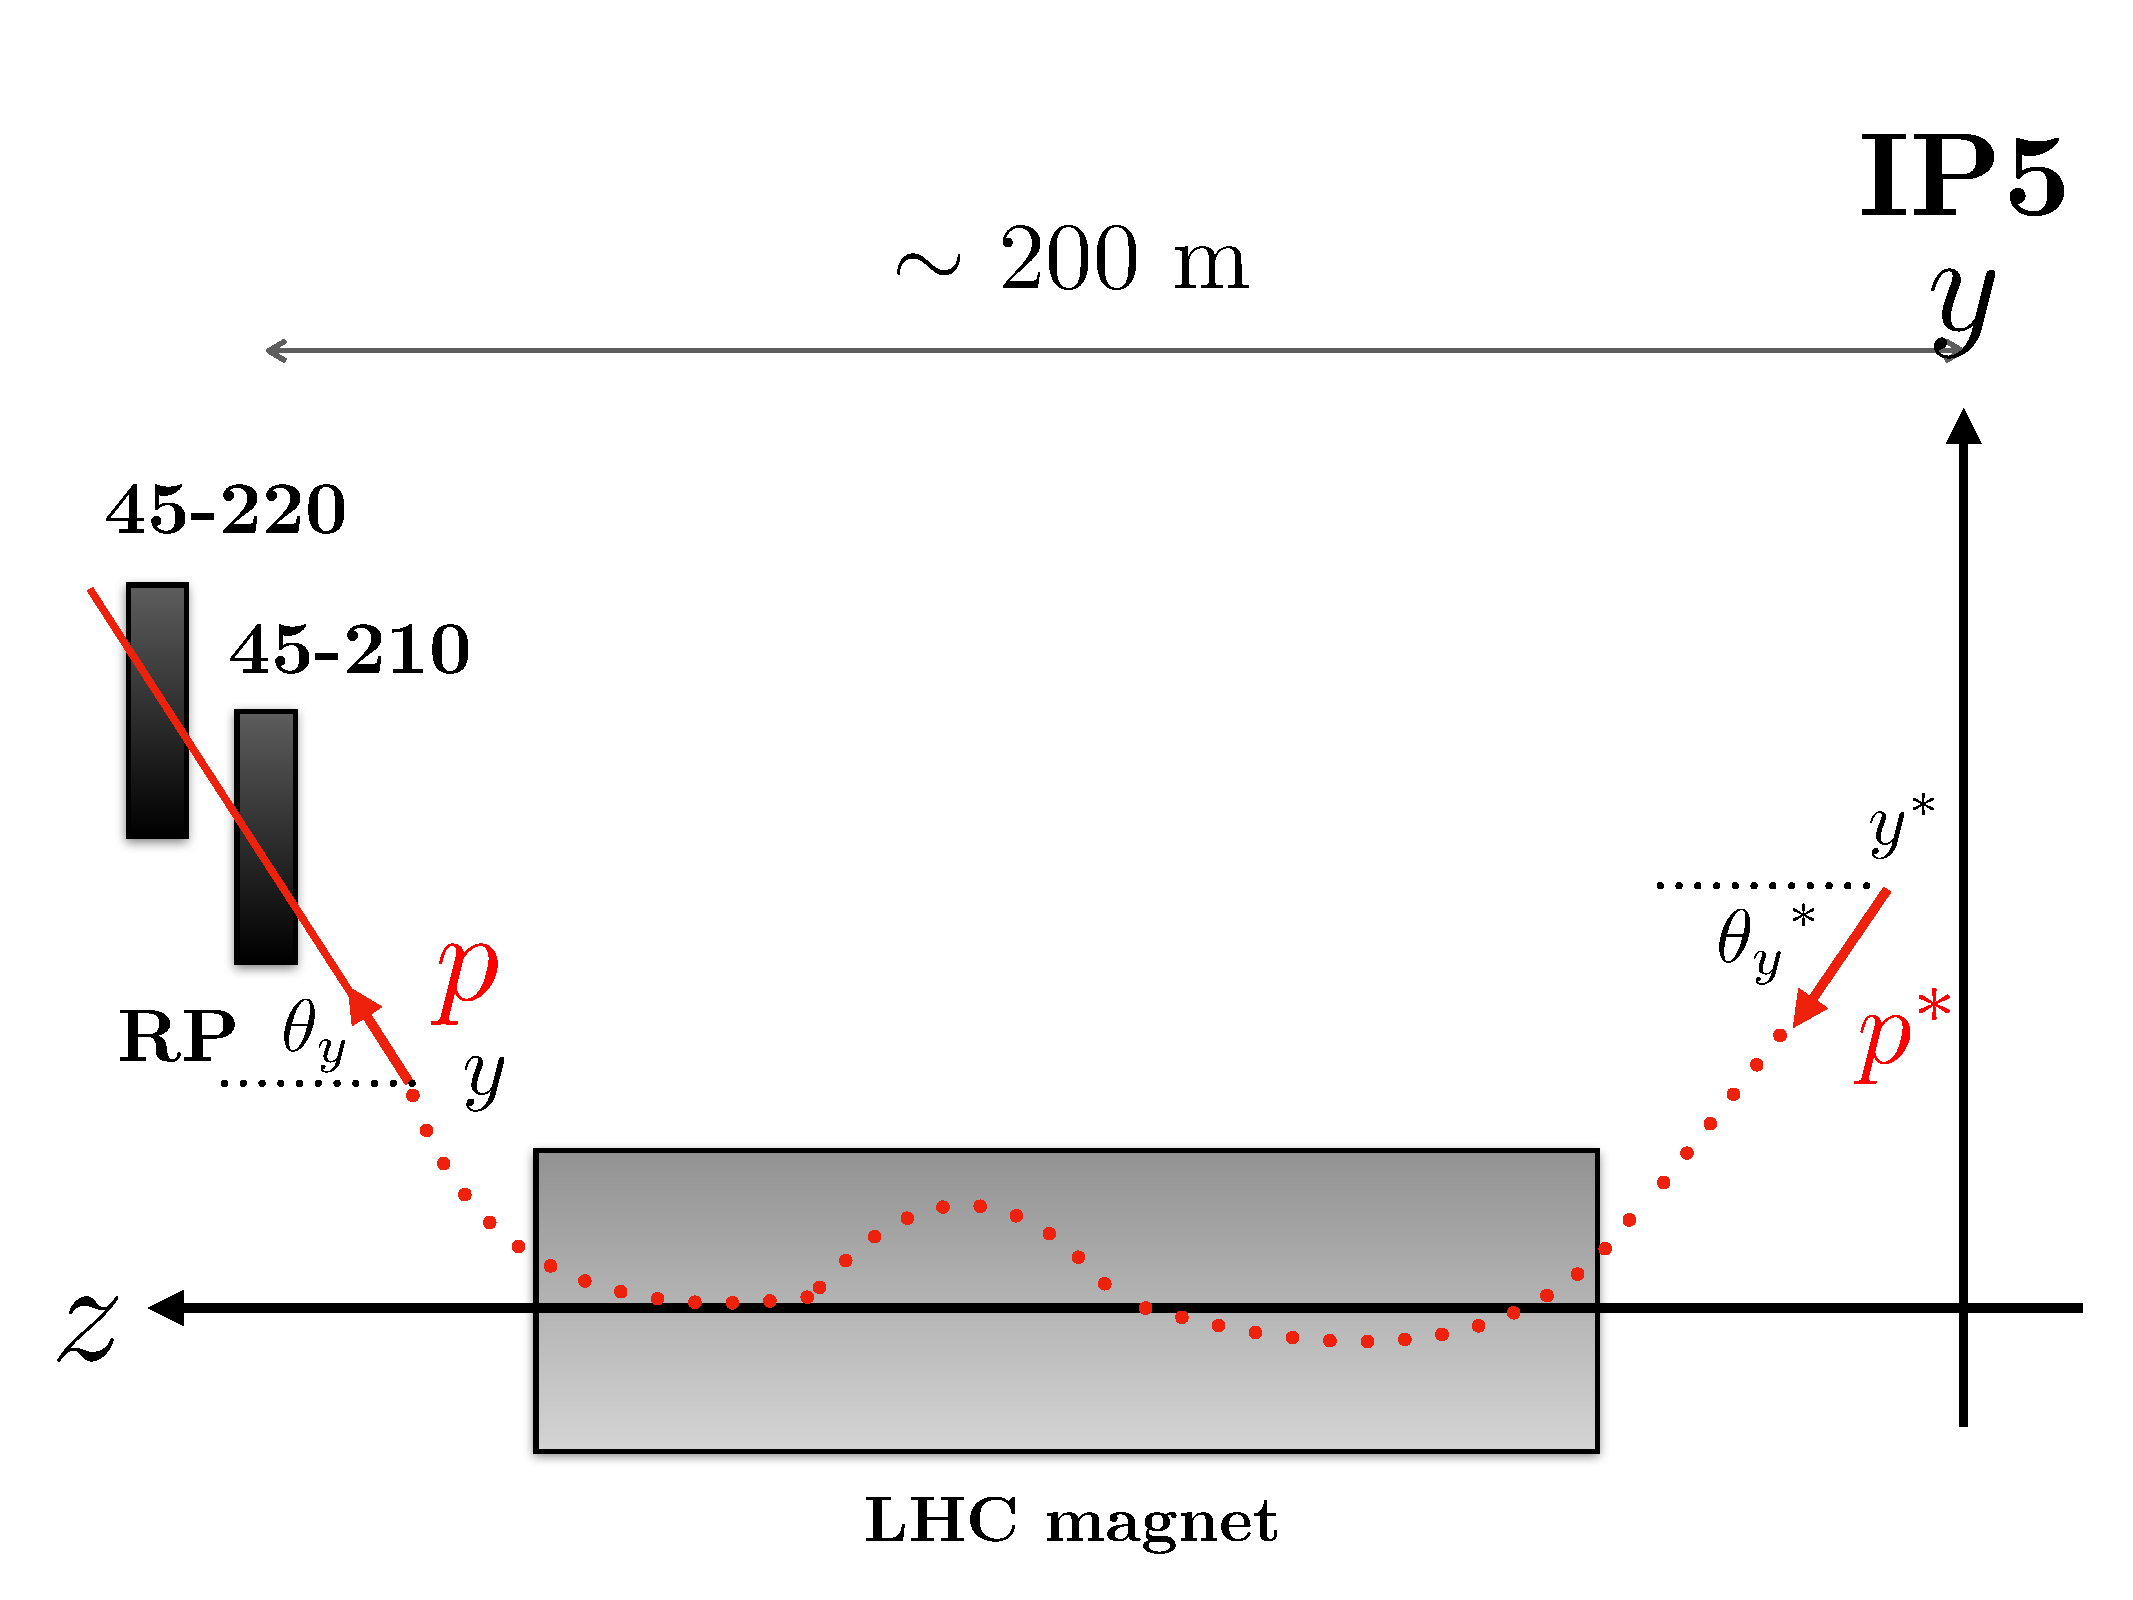
\includegraphics[scale=0.35]{protoni_RP2.pdf} 
\caption{Schema dell'evento fisico simulato. Il protone, proveniente dall'ottante 56 viene rilevato dai RP 45-210 (m) e 45-220 (m).}
\end{figure}

Le Figure 4.14 rappresentano schematicamente l'evento fisico simulato. 
Le distribuzioni che seguiranno nel prossimo paragrafo rappresentano il risultato della simulazione dei due programmi. Essi daranno in totale otto distribuzioni spaziali (quattro per ogni stazione di RP).  In particolare \'e importante osservare che le stazioni dei Roman Pot in figura sono state chiamate con nomi differenti, a seconda che i protoni scatterati proseguano il loro moto verso destra o verso sinistra rispetto all'IP5.

La simbologia utilizzata nelle due figure dovrebbe risultare molto intuitiva. Come gi\'a accennato nel Capitolo 1 e rappresentato schematicamente in Figura 1.4 LHC \'e suddiviso in ottanti (tra loro equivalenti in dimensione ma differenti in funzione e obiettivi di ricerca). CT-PPS (ossia CMS-TOTEM) \'e localizzato presso il quinto punto di interazione (IP5). Nell'urto ideale tra due protoni si assume che uno provenga dall'ottante 4 e sia diretto verso IP5 ed uno provenga dall'ottante 6 e sia diretto verso IP5. Nell'urto, il primo protone $p_1$ proseguir\'a verso l'ottante 6, mentre il secondo $p_2$ verso l'ottante 4. Ora, se aggiungiamo l'informazione che i due RP sono distanti tra loro $\sim$ 10 m (il primo a 210 m e il secondo a 220 m dall'IP), risulta ovvio il perch\'e i RP siano stati chiamati con la sigla 56-210, 56-220 e 45-210, 45-220.
Tuttavia \'e importante sottolineare che l'evento simulato dai programmi rappresenta una semplificazione della realt\'a. Infatti la disposizione dei RP \'e alquanto diversa, come \'e illustrato nelle Figure successive.

\newpage
\begin{figure}[h!] 
\centering
\includegraphics[scale=0.5]{produzione_centrale1.pdf} 
\caption{Esempio di un evento CP (Central Production) con topologia di protoni "bottom-top"; questa topologia della coppia protonica \'e simile a quella elastica (con "top-bottom" o topologia "bottom-top").}
\end{figure}

\begin{figure}[h!] 
\centering
\includegraphics[scale=0.5]{produzione_centrale2.pdf} 
\caption{Esempio di un evento CP con topologia di coppie di protoni "top-top".}
\end{figure}


Una delle sfide sperimentali \'e avere una risoluzione sufficiente per la ricostruzione del protone rilevato dai rilevatori a doppio braccio riuscendo a misurare anche le altre particelle prodotte. Nel caso di TOTEM e CMS, i due protoni principali possono essere rilevati dal sistema dei Roman Pot di TOTEM (la ricostruzione di $t_1$, $t_2$ e $\xi_1$ e $\xi_2$ utilizzando i RP \'e stata effettuata per la prima volta da TOTEM), analogamente a quanto avviene per la singola diffrazione.%\newline
  Si pu\'o quindi provare a rilevare le particelle del sistema $X$ mediante i rivelatori di CMS, come \'e possibile vedere in Figure 4.12 e 4.13 in cui sono mostrati due esempi di diversa topologia di coppia di protoni prodotta (rilevata) nei rivelatori verticali e nei rivelatori RP orizzontali. Infatti cercare i getti del sistema diffrattivo $X$ pu\'o fornire ulteriori informazioni importanti sulla struttura e la dinamica del protone.\newline
 
Nel prossimo paragrafo sono illustrate le distribuzioni spaziali dei protoni scatterati simulate da \texttt{test\_gen\_simu\_cfg.py} e  \texttt{test\_gen\_simu\_smear\_cfg.py}.
 


\newpage
\subsection{Distribuzione dei protoni (no smear)}
\begin{figure}[h] 
\centering 
\includegraphics[scale=0.47]{RP12.pdf} 
\caption{Distribuzioni dei protoni, rilevati dai Roman Pot situati a sinistra \newline (settore 45) rispetto al punto di interazione, nel caso in cui non si consideri lo smearing lungo gli assi $x$ e $y$.} 
\end{figure}
\begin{figure}[h!] 
\centering 
\includegraphics[scale=0.5]{RP2.pdf} 
\caption{Distribuzioni dei protoni, rilevati dai Roman Pot situati a destra \newline (settore 56) rispetto al punto di interazione, nel caso in cui non si consideri lo smearing lungo gli assi $x$ e $y$.} 
\end{figure}

\newpage

\subsection{Distribuzione dei protoni (smear)}
\begin{figure}[h] 
\centering 
\includegraphics[scale=0.48]{RP32.pdf} 
\caption{Distribuzioni dei protoni, rilevati dai Roman Pot situati a sinistra \newline (settore 45) rispetto al punto di interazione, nel caso in cui si consideri lo smearing lungo gli assi $x$ e $y$.} 
\end{figure}

\begin{figure}[h!] 
\centering 
\includegraphics[scale=0.45]{RP4.pdf} 
\caption{Distribuzioni dei protoni, rilevati dai Roman Pot situati a destra \newline (settore 56) rispetto al punto di interazione, nel caso in cui si consideri lo smearing lungo gli assi $x$ e $y$.} 
\end{figure}

\newpage

\subsection{Distribuzione dei protoni: no smear $vs$ smear}

\begin{figure}[h!] 
\centering 
\includegraphics[scale=0.5]{CONFRONTO1.pdf} 
\caption{Confronto tra le distribuzioni dei protoni, rilevati dai Roman Pot situati a sinistra (settore 45) rispetto al punto di interazione, nel caso in cui si consideri o meno lo smearing lungo gli assi $x$ e $y$.} 
\end{figure}
\begin{figure}[h!] 
\centering 
\includegraphics[scale=0.5]{CONFRONTO2.pdf} 
\caption{Confronto tra le distribuzioni dei protoni, rilevati dai Roman Pot situati a destra (settore 56) rispetto al punto di interazione, nel caso in cui si consideri o meno lo smearing lungo gli assi $x$ e $y$.} 
\end{figure}
\chapter*{Conclusioni}

In questo lavoro di tesi ho riportato l'attivit\'a di ricerca che ho potuto svolgere presso l'esperimento CT-PPS al Large Hadron Collider del CERN.

Nella prima parte \'e stata presentata una panoramica generale sulla fisica di LHC assieme a quella di CT-PPS, mentre nella seconda parte viene presentato il lavoro effettivamente svolto inerente alla simulazione Monte Carlo sullo scattering protone-protone assieme all'analisi dei risultati ottenuti. Riassumiamo brevemente i contenuti dell'intero elaborato.

\begin{itemize}
\item Capitolo 1: in questo capitolo \'e stato introdotto l'acceleratore LHC assieme ad una descrizione pi\'u dettagliata dell'esperimento CT-PPS (Precision Proton Spectrometer). Si \'e parlato quindi dei rivelatori utilizzati e delle condizioni sperimentali. Nella prima parte vi \'e una presentazione dei Roman Pot, mentre nella seconda \'e presentata una discussione sull'ottica del fascio, sull'accettanza e la risoluzione dei rivelatori;
\item Capitolo 2: questa parte tratta del programma di fisica dell'esperimento CT-PPS, riguardante in particolar modo i fenomeni di fisica diffrattiva (produzione centrale esclusiva $WW$, $dijets$ e collisioni a due fotoni). Nella parte finale di questo capitolo \'e stata inoltre presentata una descrizione generale ai processi elastici, diffrattivi e inelastici;
\item Capitolo 3: l'analisi della cinematica dello scattering inelastico tra protoni (in trattazione relativistica) costituisce una parte fondamentale per l'intero lavoro di tesi. Infatti \'e da questa analisi iniziale che siamo stati in grado di ricavare le espressioni delle due particlle ($X$, $Z$) originate dall'interazione dei due protoni. 

Queste, assieme al $\beta$, sono state necessarie per poter ricavate le grandezze cinematiche di nostro interesse (momento trasverso $p_T$,  componente $z$ del momento $p_z$,  momento totale $p_{tot}$, angolo di scattering $\theta$, pseudo-rapidit\'a $\eta$), le cui espressioni sono state implementate nel codice della macro di root \texttt{LorenzoGenerator.cc}.
\item Capitolo 4: nell'ultimo capitolo sono descritte e spiegate le parti pi\'u importanti del codice di \texttt{LorenzoGenerator.cc}. Abbiamo visto come l'intero codice sia suddivisibile in tre parti differenti: Generatore di eventi - Propagazione - Simulazione dei RP. 

In questa parte \'e stata inoltre discussa l'importante questione del fenomeno di smearing. Ci\'o si \'e rilevato fondamentale per una trattazione il pi\'u possibile fedele al vero. Questi effetti di smearing possono essere suddivisi in tre classi: smearing angolare (le particelle all'interno di un pacchetto non sono tutte parallele), smearing di energia (esiste una fluttuazione di energia all'interno di un pacchetto) e smearing dei vertici (le particelle hanno dimensione diversa da zero, quindi le interazioni sono distribuite nello spazio). 

Infine l'ultima parte del capitolo mostra i risultati delle simulazioni Monte Carlo generate da \texttt{LorenzoGenerator.cc}, ovvero le distribuzioni di frequenza delle grandezze cinematiche precedentemente elencate. Sono inoltre riportate le distribuzioni spaziali dei protoni rilevati dai Roman Pot generate da \texttt{test\_gen\_simu\_cfg.py} e  \texttt{test\_gen\_simu\_smear\_cfg.py}. La differenza sostanziale tra questi due \'e rappresentato dal fatto che il secondo tiene conto degli effetti di smearing (da cui il nome), mentre il primo no. La differenza tra le distribuzioni \'e alquanto macroscopica. Infatti \texttt{test\_gen\_simu\_cfg.py} origina delle tracce di protoni in prima approssimazione rettilinee, mentre invece \texttt{test\_gen\_simu\_smear\_cfg.py} genera delle distribuzioni pi\'u estese. 

Tutti questi istogrammi contribuiscono all'analisi dati portata avanti dai ricercatori di CT-PPS, ai quali spetter\'a il compito di comparare i valori sperimentali ricavati nel corso del 2017 con quelli ottenuti dalle simulazioni.
\item Appendice: in quest'ultima parte sono state inserite una serie di informazioni complementari al lavoro di tesi e che potrebbero semplificarne la lettura da parte di uno studente che non abbia mai affrontato l'analisi dati con ROOT. In questa sezione sono semplicemente introdotti alcuni dei concetti fondamentali dell'analisi dati, quali per esempio la generazione di istogrammi e il come realizzare una macro. Vi \'e inoltre un'introduzione, essenzialmente qualitativa, al concetto di simulazione Monte Carlo.
Per finire sono state inoltre riportate le distribuzioni delle grandezze cinematiche della particella $X$ e $Z$ anche nel caso in cui la massa $m_X$ valesse 800, 1000, 1400 e 1600 GeV/$c^2$.
\end{itemize}
 

\addcontentsline{toc}{chapter}{Conclusioni}
\chaptermark{Conclusioni}

%%%%%%%%%%%%%%%%%%%%%%%%%%%%%%%%%%%%%%%%%%%%

\chapter*{Ringraziamenti}
\addcontentsline{toc}{chapter}{Ringraziamenti}
\chaptermark{Ringraziamenti}
Prima di tutto, vorrei ringraziare il mio relatore di tesi N. Turini e S. Giani per avermi permesso di trascorrere l'estate presso il CERN. Un grazie speciale \'e rivolto anche ai colleghi che ho incontrato durante il mio tirocinio. In particolare, mi rivolgo a Jan Kaspar per avermi aiutato nella stesura del codice, a Edoardo Bossini, Andrea Bellora e Nicola Minafra per avermi guidato nei momenti di smarrimento e per i loro preziosi consigli. Un sentito grazie \'e inoltre rivolto a Gaia e Oriol, che hanno reso indimenticabile il mio soggiorno a Ginevra.  \newline
Vorrei adesso ringraziare tutti coloro che hanno contribuito a rendere pi\'u piacevoli questi tre anni. Grazie a tutti i ragazzi con i quali ho condiviso le ore di lezione e di studio, spero vivamente di rincontrarvi in futuro e grazie ad Antonietta, per avermi offerto il miglior soggiorno che uno studente possa avere. \newline
Dedico inoltre questo giorno alla professoressa G. Righi e il professor G. Gargani, grazie ai quali mi sono inscritto a Fisica.\newline
Seguire i corsi e preparare gli esami non \'e sufficiente per riuscire a laurearsi. Per me \'e stato di fondamentale importanza essere circondato da amici e persone che ogni giorno mi hanno dimostrato affetto e con i quali ho condiviso momenti di spensieratezza e divertimento. Ringrazio quindi il Menca per la sua rara sensibilti\'a e per il suo altruismo, Niccol\'o, il matematico pi\'u brillante che conosca, Antonio, per le domeniche passate insieme a suonare e Arianna, la mia ultima scoperta.
Questo giorno rappresenta un omaggio a tutti coloro che hanno sempre creduto in me e a tale proposito ringrazio il $Cocco$ per aver fatto quella telefonata, e Federico per avermi indirizzato al meglio.
Ovviamente un ringraziamento speciale \'e rivolto a tutta la mia famiglia e in particolare a mia madre, per aver sempre sostenuto sia le mie scelte che (soprattutto) le mie spese.
Infine voglio dedicare questo traguardo ad una persona che ha profondamente segnato la mia esistenza e che se fosse qui sarebbe fiero di me. Per te Babbo!

%%%%%%%%%%%%%%%%%%%%%%%%%%%%%%%%%%%%%%%%%%%%

\chapter*{Appendice}
\addcontentsline{toc}{chapter}{Appendice}
\chaptermark{Appendice}
\section{Analisi dati con ROOT}
\subsection{Motivazione e Introduzione}
La comparazione delle misurazioni con i modelli teorici \'e uno dei compiti standard nella fisica sperimentale. Nei casi pi\'u semplici, un "modello" \'e soltanto una funzione che fornisce previsioni di dati misurati e molto spesso il modello dipende da certi parametri.
\newline
Come primo step, \'e necessaria una visualizzazione dei dati. Dopo di che, alcune manipolazioni devono tipicamente essere applicate, per esempio correzioni o trasformazioni dei parametri.
\newline
Una specialit\'a della fisica sperimentale sono le inevitabili incertezze da cui ciascuna misurazione \'e affetta, ed \'e dunque necessario che nelle analisi dei dati la natura statistica degli errori venga gestita in modo corretto. Come ultimo passo, le misure devono essere comparate ai modelli, e i parametri liberi devono essere determinati in questo processo. Sono quindi richiesti strumenti per generare e visualizzare distribuzioni di frequenza (istogrammi), e un rigoroso trattamento statistico per estratte i parametri del modello da distribuzioni puramente statistiche.
\newline

La simulazione dei dati attesi \'e un altro aspetto importante dell'analisi dati. Attraverso la generazione ripetuta di "pseudo-data", i quali sono analizzati nello stesso modo previsto per i dati reali, le procedure di analisi possono essere tra loro comparate. In molti casi la distribuzione degli errori di misurazione non \'e ben nota, e la simulazione offre la possibilit\'a di testare gli effetti di assunzioni differenti.

Un potente software in grado di soddisfare tuti i requisiti appena elencati \'e \index{ROOT}, un progetto open source (libero per molte piattaforme come LInux, Mac OS X, Windows...) coordinato dal CERN. ROOT, scritto e basato sulla programmazione in linguaggio  \texttt{C++}, \'e molto flessibile e fornisce sia un interfaccia di programmazione sia un interfaccia grafico, per un'analisi dei dati interattiva.
\newline
Le informazioni che seguiranno sono prese dalle guide ufficiali consultabili in rete [17].
\newline

\subsection{Istogrammi con ROOT}
Come appena accennato, sono moltissime le funzioni e gli strumenti messi a disposizione da ROOT. Esso infatti pu\'o essere utilizzato semplicemente come una calcolatrice, per plottare funzioni, per plottare misurazioni, oppure per rappresentare distribuzioni di frequenza, ossia istogrammi.

Gli istogrammi e i numeri random sono degli strumenti molto importanti nell'analisi statistica dei dati. Gli istogrammi in ROOT sono gestiti da un insieme di classi provenienti dalla classe \texttt{TH1}. Generalmente si utilizza la classe \texttt{TH1F}, dove la lettera \texttt{F} sta per "float", che significa che il dato di tipo \texttt{float} \'e utilizzato per memorizzare le entrate in un bin dell'istogramma. 

Quando vogliamo rappresentare distribuzioni di frequenza dobbiamo utilizzare anche un'altra funzionalit\'a di ROOT, per riempire istogramma con dei dati, chiamati pseudo-random numbers generated. Ci\'o viene realizzato con il metodo \texttt{TF1::GetRandom}, il quale a sua volta \'e una istanza della classe \texttt{TRandom}.
\newline
I dati sono inseriti nell'istogramma utilizzando il metodo \texttt{TH1F::Fill} attraverso un costrutto ciclico (\texttt{ciclo for}). Come risultato di tutto ci\'o, l'istogramma \'e riempito con un certo numero arbitrario e prestabilito (generalmente 1000) di numeri random distribuiti secondo la funzione definita. Per finire, l'istogramma \'e rappresentato utilizzando il metodo \texttt{TH1F::Draw()}. Ovviamente, nel ripetere la generazione di un nuovo istogramma, non ne otterremo mai uno uguale all'altro, essendo questi dipendenti da come viene inizializzato il generatore di numeri casuali.

\subsection{Macro di ROOT}
Compilare una macro, o un'applicazione indipendente, \'e relativamente semplice in ROOT. Se noi abbiamo un numero di linee di codice che siano in grado di eseguire una richiesta, queste possono essere raccolte in una macro semplicemente dando loro un nome, il quale corrisponde al nome del file senza estensione.
La struttura generale per una macro memorizzata in un file chiamato \texttt{MacroName.C} \'e \newline

\texttt{void MacroName()} \hspace{1cm} \texttt{$\{$}\newline
\texttt{...} \hspace{1cm} \texttt{linee}  \texttt{di}  \texttt{codice} \texttt{in} \texttt{C++} \hspace{1cm} \texttt{...} \newline
\texttt{$\}$}\newline


La macro \'e eseguita digitando \newline

\texttt{$>$} \texttt{root} \texttt{[0]} \texttt{MacroName.C} \newline

o in alternativa\newline

\texttt{$>$} \texttt{root} \texttt{[0]} \texttt{.x} \texttt{MacroName.C} \newline



\subsection{Simulazione Monte Carlo}
Molto spesso \'e necessario studiare le propriet\'a statistiche delle procedure di analisi. Questo \'e raggiunto pi\'u facilmente applicando le analisi a molti gruppi di dati simulati (o "pseudo-dati"), ognuno dei quali rappresenta una possibile versione del vero esperimento. Se la distribuzione riguarda solo la distribuzione finale osservata nei dati, e non si esegue una simulazione completa della fisica sottostante e dell'apparecchiatura sperimentale, si utilizza frequentemente il Toy Monte Carlo\footnote{Il termine simulazione Monte Carlo fu coniato all'inizio della seconda guerra mondiale da von Neumann e Ulam a Los Alamos, che studiavano la dinamica delle esplosioni nucleari nell'ambito del progetto Manhattan.Il nome fu ispirato alla casualit\'a dei risultati nelle case da gioco dei Casin\'o di Monte Carlo.}.\newline

La principale motivazione all'uso di simulazioni Monte Carlo consiste nel fatto che in un tipico esperimento di fisica delle particelle le quanti\'a fisiche da misurare sono basate su processi casuali. Risulta quindi fondamentale conoscere la natura di questi processi e riprodurre il singolo processo al calcolatore.\newline
Non solo, anche l'apparato sperimentale utilizzato per un certo esperimento pu\'o distorcere l'evento fisico considerato. Potremmo quindi chiederci: quali sono i processi fisici che avvengono all'interno dell'apparato? Con quale probabilit\'a avvengono? Come si calcola l'accettanza (numero di eventi di un certo tipo misurabili dall'apparato sul totale degli eventi di quel tipo) dell'apparato?

Il metodo Monte Carlo d\'a una risposta a queste domande e si basa sulla disponibilit\'a di sequenze casuali\footnote{I generatori di sequenze pseudo-casuali sono in realt\'a degli algoritmi che generano sequenze di numeri che sembrano a tutti gli effetti casuali.} di numeri (donde il nome), distribuiti uniformemente tra 0 e 1.\newline

Esistono tecniche statistiche che consentono di utilizzare queste sequenze per campionare processi aventi distribuzioni di probabilit\'a di forma qualsiasi. Per esempio, se conosciamo la vita media di una particella possiamo simularne il decadimento, campionando una distribuzione esponenziale decrescente avente come parametro la vita media della particella.
Con queste tecniche si possono quindi simulare i processi di propagazione delle particelle nei materiali e le risposte dei rivelatori al passaggio della radiazione.
\section{Istogrammi}
Come gi\'a affermato all'inizio del capitolo 4, le simulazioni sono state implementate per diversi casi, a seconda del valore attribuito alla massa della particella $X$. Quindi in totale sono state effettuate sei simulazioni diverse, nelle quali la massa della particella $X$ assumeva i valori $m_X$ = 800, 1000, 1200, 1400, 1600 GeV/$c^2$. Il caso intermedio \newline($m_X$ = 1.2 TeV/$c^2$) \'e gi\'a stato analizzato precedentemente, mentre invece le distribuzioni degli altri casi sono riportati di seguito, in ordine crescente di massa. 
\clearpage
\newpage
\begin{figure}
\begin{minipage}[t]{8.5cm}
\centering
\includegraphics[width=9cm]{p_T_X_800.pdf}
%\caption{Prima figura}
\end{minipage}
\ \hspace{1mm} \hspace{1mm} \
\begin{minipage}[t]{8.5cm}
\centering
\includegraphics[width=9cm]{p_T_Z_800.pdf}
%\caption{Seconda figura}
\end{minipage}
\end{figure}

\begin{figure}
\begin{minipage}[b]{8.5cm}
\centering
\includegraphics[width=9cm]{p_z_X_800.pdf}
%\caption{Prima figura}
\end{minipage}
\ \hspace{1mm} \hspace{1mm} \
\begin{minipage}[b]{8.5cm}
\centering
\includegraphics[width=9cm]{p_z_Z_800.pdf}
%\caption{Seconda figura}
\end{minipage}
\end{figure}

\begin{figure}
\begin{minipage}[h!]{8.5cm}
\centering
\includegraphics[width=9cm]{p_tot_X_800.pdf}
%\caption{Prima figura}
\end{minipage}
\ \hspace{1mm} \hspace{1mm} \
\begin{minipage}[h!]{8.5cm}
\centering
\includegraphics[width=9cm]{p_tot_Z_800.pdf}
%\caption{Seconda figura}
\end{minipage}
\end{figure}

\begin{figure}
\begin{minipage}[h!]{8.5cm}
\centering
\includegraphics[width=9cm]{Theta_X_800.pdf}
%\caption{Prima figura}
\end{minipage}
\ \hspace{1mm} \hspace{1mm} \
\begin{minipage}[h!]{8.5cm}
\centering
\includegraphics[width=9cm]{Theta_Z_800.pdf}
%\caption{$m_X$ = 800 GeV}
\end{minipage}
\end{figure}

\begin{figure}
\begin{minipage}[h!]{8.5cm}
\centering
\includegraphics[width=9cm]{Eta_X_800.pdf}
\caption{$m_X$ = 800 GeV/$c^2$}
\end{minipage}
\ \hspace{1mm} \hspace{1mm} \
\begin{minipage}[h!]{8.5cm}
\centering
\includegraphics[width=9cm]{Eta_Z_800.pdf}
\caption{$m_Z$ = 91 GeV/$c^2$}
\end{minipage}
\end{figure}

\clearpage
\newpage


\begin{figure}
\begin{minipage}[h!]{8.5cm}
\centering
\includegraphics[width=9cm]{p_T_X_1000.pdf}
%\caption{Prima figura}
\end{minipage}
\ \hspace{1mm} \hspace{1mm} \
\begin{minipage}[h!]{8.5cm}
\centering
\includegraphics[width=9cm]{p_T_Z_1000.pdf}
%\caption{Seconda figura}
\end{minipage}
\end{figure}

\begin{figure}
\begin{minipage}[h!]{8.5cm}
\centering
\includegraphics[width=9cm]{p_z_X_1000.pdf}
%\caption{Prima figura}
\end{minipage}
\ \hspace{1mm} \hspace{1mm} \
\begin{minipage}[h!]{8.5cm}
\centering
\includegraphics[width=9cm]{p_z_Z_1000.pdf}
%\caption{Seconda figura}
\end{minipage}
\end{figure}

\begin{figure}
\begin{minipage}[h!]{8.5cm}
\centering
\includegraphics[width=9cm]{p_tot_X_1000.pdf}
%\caption{Prima figura}
\end{minipage}
\ \hspace{1mm} \hspace{1mm} \
\begin{minipage}[h!]{8.5cm}
\centering
\includegraphics[width=9cm]{p_tot_Z_1000.pdf}
%\caption{Seconda figura}
\end{minipage}
\end{figure}

\begin{figure}
\begin{minipage}[h!]{8.5cm}
\centering
\includegraphics[width=9cm]{Theta_X_1000.pdf}
%\caption{Prima figura}
\end{minipage}
\ \hspace{1mm} \hspace{1mm} \
\begin{minipage}[h!]{8.5cm}
\centering
\includegraphics[width=9cm]{Theta_Z_1000.pdf}
%\caption{Seconda figura}
\end{minipage}
\end{figure}

\begin{figure}
\begin{minipage}[h!]{8.5cm}
\centering
\includegraphics[width=9cm]{Eta_X_1000.pdf}
\caption{$m_X$ = 1000 GeV/$c^2$}
\end{minipage}
\ \hspace{1mm} \hspace{1mm} \
\begin{minipage}[h!]{8.5cm}
\centering
\includegraphics[width=9cm]{Eta_Z_1000.pdf}
\caption{$m_Z$ = 91 GeV/$c^2$}
\end{minipage}
\end{figure}



\begin{figure}
\begin{minipage}[h!]{8.5cm}
\centering
\includegraphics[width=9cm]{p_T_X_1400.pdf}
%\caption{Prima figura}
\end{minipage}
\ \hspace{1mm} \hspace{1mm} \
\begin{minipage}[h!]{8.5cm}
\centering
\includegraphics[width=9cm]{p_T_Z_1400.pdf}
%\caption{Seconda figura}
\end{minipage}
\end{figure}

\begin{figure}
\begin{minipage}[h!]{8.5cm}
\centering
\includegraphics[width=9cm]{p_z_X_1400.pdf}
%\caption{Prima figura}
\end{minipage}
\ \hspace{1mm} \hspace{1mm} \
\begin{minipage}[h!]{8.5cm}
\centering
\includegraphics[width=9cm]{p_z_Z_1400.pdf}
%\caption{Seconda figura}
\end{minipage}
\end{figure}

\begin{figure}
\begin{minipage}[h!]{8.5cm}
\centering
\includegraphics[width=9cm]{p_tot_X_1400.pdf}
%\caption{Prima figura}
\end{minipage}
\ \hspace{1mm} \hspace{1mm} \
\begin{minipage}[h!]{8.5cm}
\centering
\includegraphics[width=9cm]{p_tot_Z_1400.pdf}
%\caption{Seconda figura}
\end{minipage}
\end{figure}

\begin{figure}
\begin{minipage}[h!]{8.5cm}
\centering
\includegraphics[width=9cm]{Theta_X_1400.pdf}
%\caption{Prima figura}
\end{minipage}
\ \hspace{1mm} \hspace{1mm} \
\begin{minipage}[h!]{8.5cm}
\centering
\includegraphics[width=9cm]{Theta_Z_1400.pdf}
%\caption{Seconda figura}
\end{minipage}
\end{figure}

\begin{figure}
\begin{minipage}[h!]{8.5cm}
\centering
\includegraphics[width=9cm]{Eta_X_1400.pdf}
\caption{$m_X$ = 1400 GeV/$c^2$}
\end{minipage}
\ \hspace{1mm} \hspace{1mm} \
\begin{minipage}[h!]{8.5cm}
\centering
\includegraphics[width=9cm]{Eta_Z_1400.pdf}
\caption{$m_Z$ = 91 GeV/$c^2$}
\end{minipage}
\end{figure}


\begin{figure}
\begin{minipage}[h!]{8.5cm}
\centering
\includegraphics[width=9cm]{p_T_X_1600.pdf}
%\caption{Prima figura}
\end{minipage}
\ \hspace{1mm} \hspace{1mm} \
\begin{minipage}[h!]{8.5cm}
\centering
\includegraphics[width=9cm]{p_T_Z_1600.pdf}
%\caption{Seconda figura}
\end{minipage}
\end{figure}

\begin{figure}
\begin{minipage}[h!]{8.5cm}
\centering
\includegraphics[width=9cm]{p_z_X_1600.pdf}
%\caption{Prima figura}
\end{minipage}
\ \hspace{1mm} \hspace{1mm} \
\begin{minipage}[h!]{8.5cm}
\centering
\includegraphics[width=9cm]{p_z_Z_1600.pdf}
%\caption{Seconda figura}
\end{minipage}
\end{figure}

\begin{figure}
\begin{minipage}[h!]{8.5cm}
\centering
\includegraphics[width=9cm]{p_tot_X_1600.pdf}
%\caption{Prima figura}
\end{minipage}
\ \hspace{1mm} \hspace{1mm} \
\begin{minipage}[h!]{8.5cm}
\centering
\includegraphics[width=9cm]{p_tot_Z_1600.pdf}
%\caption{Seconda figura}
\end{minipage}
\end{figure}

\begin{figure}
\begin{minipage}[h!]{8.5cm}
\centering
\includegraphics[width=9cm]{Theta_X_1600.pdf}
%\caption{Prima figura}
\end{minipage}
\ \hspace{1mm} \hspace{1mm} \
\begin{minipage}[h!]{8.5cm}
\centering
\includegraphics[width=9cm]{Theta_Z_1600.pdf}
%\caption{Seconda figura}
\end{minipage}
\end{figure}

\begin{figure}
\begin{minipage}[h!]{8.5cm}
\centering
\includegraphics[width=9cm]{Eta_X_1600.pdf}
\caption{$m_X$ = 1600 GeV/$c^2$}
\end{minipage}
\ \hspace{1mm} \hspace{1mm} \
\begin{minipage}[h!]{8.5cm}
\centering
\includegraphics[width=9cm]{Eta_Z_1600.pdf}
\caption{$m_Z$ = 91 GeV/$c^2$}
\end{minipage}
\end{figure}


 \addcontentsline{toc}{chapter}{Bibliografia} \clearpage
\begin{thebibliography}{99}
%\bibitem{Mazzoldi, Nigro, Voci} P. Mazzoldi, M. Nigro, C. Voci - "Fisica 2" - Edises \bibitem{elettronica} Millman - "Elettronica" - McGraw-Hill
\bibitem {errori} $Large$$Hadron$$Collider$, From Wikipedia the free encyclopedia $http://en. wikipedia.org/wiki/LHC$
\bibitem GG. Antchev et al. [TOTEM Collaboration], "LHC optics measurement with proton tracks detected by the roman pots of the TOTEM experiment", arXiv:1406.0546 [physics.acc-ph].
\bibitem AA.LatinaandL.Deniau,"EvolutionofMAD-XintheFrameworkofLHCUpgradeStudies",Conf. Proc. C 1205201, 304 (2012).
\bibitem JJ. Favereau de Jeneret, X. Rouby, K. Piotrzkowski, JINST 2 (2007) P09005; arXiv:0707.1198.
\bibitem MM. Benedikt, P. Collier, V. Mertens, J. Poole and K. Schindl, ?LHC Design Report. 3. The LHC injector chain?, CERN-2004-003-V-3.
\bibitem  CCCMS-TOTEM Precision Proton Spectrometer Technical Design Report, CERN-LHCC-2014-021
\bibitem JJ. Kaspar, "Elastic scattering at the LHC", Ph.D. thesis, CERN-THESIS-2011-214.
\bibitem TT. Aaltonen et al. [CDF Collaboration], "Observation of exclusive dijet production at the Fermilab
Tevatron pp "Collider", Phys. Rev. D 77, 052004 (2008), [arXiv:0712.0604 [hep-ex]].
\bibitem SS. Chatrchyan et al. [CMS Collaboration], "Observation of a diffractive contribution to dijet
production in proton-proton collisions at s = 7 TeV", Phys. Rev. D 87, 012006 (2013), [arXiv:1209.1805 [hep-ex]].
\bibitem TTOTEM Collaboration, TOTEM Upgrade Proposal, CERN-LHCC-2013-009; LHCC-P-007 and "Timing Measurements in the Vertical Roman Pots of the TOTEM Experiment", CERN-LHCC- 2014-020 (TOTEM-TDR-002).
\bibitem "Installation of Physics Debris Absorbers (TCL) on both sides of IP1 and IP5 in front of Q6 Quadrupole", LHC-LJ-EC-0040, EDMS 1357736.
\bibitem AA. Lapertosa, "Analisi preliminare sui dati relativi al tracciatore T2 dell'esperimento TOTEM a LHC", Tesi di Laurea triennale.
\bibitem TThe CMS and TOTEM diffractive and forward physics working group, "Prospects for Diffractive and Forward Physics at the LHC", CERN/LHCC 2006-039/G-124 (2006).
\bibitem SSee e.g. M.G. Albrow, T.D. Coughlin, and J.R. Forshaw, Prog. Part. Nucl. Phys. 65 (2010) 149.
\bibitem KK. Piotrzkowski, "Tagging Two-Photon Production at the LHC", Phys. Rev. D 63, 071502(R).
\bibitem  DD.d'Enterria and G.G.Silveira, "Observing light-by-light scattering at the Large Hadron Collider", Phys.Rev.Lett. 111 (2013) 080405
\bibitem TThe Root Reference Guide 2013 http://root.cern.ch/downloading-root.
\end{thebibliography}
%%%%%%%%%%%%%%%%%%%%%%%%%%%%%%%%%%%%%%%%%%%%
 %%%%%%%%%%%%%%%%%%%%%%%%%%%%%%%%%%%%%%%%%%%%
%\addcontentsline{toc}{chapter}{\indexname} \printindex
\end{document}
